% !TEX program = xelatex
% ---------------------------------------------------------------------------
%  BlackHoleSimulator -- companion paper
%  Build:  tectonic -X compile paper.tex --outdir .
% ---------------------------------------------------------------------------
\documentclass[11pt,a4paper,fontset=windows]{ctexart}

\usepackage[a4paper,top=2.4cm,bottom=2.4cm,left=2.3cm,right=2.3cm]{geometry}
\usepackage{amsmath,amssymb,amsthm}
\usepackage{graphicx}
\usepackage{booktabs}
\usepackage{array}
\usepackage{multirow}
\usepackage{longtable}
\usepackage{caption}
\usepackage{subcaption}
\usepackage{xcolor}
\usepackage{listings}
\usepackage{enumitem}
\usepackage{float}
\usepackage{placeins}
% Long file paths and command lines appear throughout the appendix and the
% implementation section.  A plain \texttt{} box cannot be broken at all, so a
% single 40-character path can force an overfull line.  xurl (a thin wrapper
% around url) makes those tokens breakable while keeping the typewriter face,
% and \path{} drops out of the hyperref machinery cleanly.  It has to be loaded
% next to hyperref; both orders work, this one keeps the url machinery first.
\usepackage{xurl}
\usepackage[hidelinks,unicode]{hyperref}

\graphicspath{{figures/}{figures/png/}}

\captionsetup{font=small,labelfont=bf,skip=5pt}
\captionsetup[sub]{font=footnotesize}

% The bibliography uses author-year labels, so every citation is a long
% unbreakable box (``[Chandrasekhar(1983)]'' and worse).  A line that has to
% absorb one of those boxes, with the CJK glue around it, can leave the
% breaker with no feasible break point at the default tolerance, and TeX then
% emits a badly overfull line.  A small emergency stretch gives the breaker
% room to loosen a line instead; it is only used when nothing else works.
\emergencystretch=3em

% -- code listings ----------------------------------------------------------
\definecolor{cmt}{RGB}{110,120,130}
\definecolor{kw}{RGB}{150,40,120}
\definecolor{str}{RGB}{40,110,80}
\definecolor{bg}{RGB}{248,248,250}
\lstdefinestyle{glsl}{
  basicstyle=\ttfamily\scriptsize,
  backgroundcolor=\color{bg},
  commentstyle=\color{cmt}\itshape,
  keywordstyle=\color{kw}\bfseries,
  stringstyle=\color{str},
  numbers=left, numberstyle=\tiny\color{cmt}, numbersep=6pt,
  frame=single, rulecolor=\color{cmt!40}, framesep=4pt,
  breaklines=true, showstringspaces=false, tabsize=2,
  columns=fullflexible, keepspaces=true, upquote=true,
}
\lstset{style=glsl}

% The five inline listings in the body and the seven floating listings in
% the appendix form one single sequence in the text, so they must share
% both the counter and the label.  The \texttt{listings} package defaults
% to the English word ``Listing''; the float defined below already uses
% the Chinese name, and leaving the default would print two different
% labels for the same kind of object.
\renewcommand{\lstlistingname}{代码}
\renewcommand{\lstlistlistingname}{代码索引}

% A float that can carry a listings body plus a Chinese caption.  The
% listings package does not define a float of its own, and putting the
% caption inside \lstinputlisting's option list would typeset it in the
% listing font, where the CJK range has no glyphs.  Defining the float
% explicitly keeps the caption in the normal caption font.
\floatstyle{ruled}
\newfloat{listing}{tbp}{lol}
\floatname{listing}{代码}

% Two of the appendix tables are symbol and artefact indices.  They are set
% as longtables because they have to break across pages, but their titles
% say explicitly that they are auxiliary material outside the numbered
% sequence of the text.  A longtable steps the shared `table' counter even
% when it carries no caption (it has to, so that \caption keeps working
% inside it), and that step would silently shift the number of every table
% typeset after the index.  \auxkeepcounter saves the counter and parks it
% on a value far above the range the paper uses, so that the index neither
% consumes a number nor re-uses a number -- and therefore neither the
% printed numbers nor hyperref's named destinations of the real tables are
% affected; \auxrestorecounter puts the counter back afterwards.
\newcounter{auxsavetable}
\newcommand{\auxkeepcounter}[1]{%
  \setcounter{auxsavetable}{\value{table}}%
  \setcounter{table}{#1}}
\newcommand{\auxrestorecounter}{\setcounter{table}{\value{auxsavetable}}}

% The Tectonic bundle ships only a subset of listings' language drivers
% (\texttt{java} is present, \texttt{JavaScript}/\texttt{CSS}/\texttt{GLSL}
% are not), so the three languages used in this paper are defined here.
% Keeping them local also makes the build independent of the TeX Live
% snapshot the reader happens to have installed.
\lstdefinelanguage{GLSL}{
  morekeywords={attribute,const,uniform,varying,buffer,layout,centroid,flat,
    smooth,noperspective,patch,sample,break,continue,do,for,while,switch,
    case,default,if,else,in,out,inout,float,double,int,uint,void,bool,true,
    false,discard,return,precision,lowp,mediump,highp,struct,vec2,vec3,vec4,
    ivec2,ivec3,ivec4,bvec2,bvec3,bvec4,uvec2,uvec3,uvec4,mat2,mat3,mat4,
    mat2x2,mat2x3,mat2x4,mat3x2,mat3x3,mat3x4,mat4x2,mat4x3,mat4x4,
    sampler2D,sampler3D,samplerCube,sampler2DArray,isampler2D,usampler2D},
  sensitive=true,
  morecomment=[l]{//},
  morecomment=[s]{/*}{*/},
  morestring=[b]"
}
\lstdefinelanguage{JavaScript}{
  morekeywords={break,case,catch,class,const,continue,default,delete,do,else,
    export,extends,finally,for,function,if,import,in,instanceof,let,new,of,
    return,static,super,switch,this,throw,try,typeof,var,void,while,yield,
    async,await,true,false,null,undefined},
  sensitive=true,
  morecomment=[l]{//},
  morecomment=[s]{/*}{*/},
  morestring=[b]',
  morestring=[b]",
  morestring=[b]`
}
\lstdefinelanguage{CSS}{
  morekeywords={display,position,flex,grid,width,height,margin,padding,
    border,background,color,font,opacity,transition,transform,overflow,
    content,top,left,right,bottom,cursor,pointer,none,absolute,relative,
    fixed,hidden,auto,block,inline,inherit},
  sensitive=false,
  morecomment=[s]{/*}{*/},
  morestring=[b]',
  morestring=[b]"
}

% -- math shorthands --------------------------------------------------------
\newcommand{\M}{M}
\newcommand{\dd}{\mathrm{d}}
\newcommand{\ie}{\emph{i.e.}}
\newcommand{\eg}{\emph{e.g.}}
\newcommand{\rs}{r_{\mathrm s}}
\newcommand{\bin}{r_{\mathrm{in}}}
\newcommand{\bout}{r_{\mathrm{out}}}
\newcommand{\bisco}{r_{\mathrm{ISCO}}}
\newcommand{\bph}{r_{\mathrm{ph}}}
\newcommand{\bc}{b_{c}}
\newcommand{\gfac}{g}
\newcommand{\lcdm}{\Lambda\text{CDM}}
\newcommand{\Msun}{M_{\odot}}

\theoremstyle{plain}
\newtheorem{proposition}{命题}
\newtheorem{lemma}{引理}
\theoremstyle{definition}
\newtheorem{remark}{注记}

\hypersetup{
  pdftitle={施瓦西黑洞实时成像模拟器：物理建模、数值方法与 GPU 实现},
  pdfauthor={徐上（无锡工艺职业技术学院）},
  pdfsubject={相对论天体物理，数值相对论，实时光线追踪},
  pdfkeywords={黑洞，施瓦西度规，零测地线，吸积盘，Page-Thorne，WebGL，GPU},
}

\title{\bfseries 施瓦西黑洞实时成像模拟器\\[6pt]
\large 物理建模、数值方法、GPU 实现与实验验证}
\author{徐上\\[3pt]
\normalsize 无锡工艺职业技术学院\\[3pt]
\small\ttfamily 3473945423@qq.com \quad 15366192183\\[3pt]
\small\ttfamily https://github.com/AaronShawn/blackhole-simulator\\[1pt]
\small（项目已开源）}
\date{2026 年 9 月}

\begin{document}
\maketitle

\begin{abstract}
\noindent
本文给出一个可在普通消费级显卡上实时运行的施瓦西黑洞成像模拟器，并从广义相对论、
广义相对论辐射转移、数值分析与计算机图形学四个层面给出完整的建模、推导、实现与实验验证。
模拟器在每一个像素上求解由施瓦西度规导出的零测地线方程
$\dd^2u/\dd\varphi^2=-u+3\M u^2$（$u\equiv1/r$），采用经典四阶 Runge--Kutta 积分器与
几何自适应步长，同时输出临界冲击参数 $\bc=3\sqrt3\,\M$、光子球半径 $\bph=3\M$
与视界阴影角半径的解析对照量。吸积盘采用 Page--Thorne（1974）广义相对论薄盘通量剖面，
并在运行时与 Shakura--Sunyaev（1973）牛顿近似剖面做定量对照；盘内辐射经过前向累积的
体积辐射转移、相对论频移 $g$ 与 $I\propto g^{4}$ 集束律、以及基于 CIE 1931 色度轨迹的
黑体配色后进入 HDR 累积—辉光—ACES 影调映射管线。为保证“物理正确”而非“视觉近似”，
本文报告了六组独立验证实验（V1--V6），把着色器输出与解析解或双精度 CPU 参考实现逐点比对：
临界冲击参数相对误差 $1.0\times10^{-14}$；近临界轨道的积分守恒误差在 $tol=3\times10^{-4}$
处触底于 $2.6\times10^{-6}$；阴影半径的亚像素反解与闭式相符到 $6.5\times10^{-12}$；
界面内建的实时测量在 $1440\times820$ 下给出 $144.73$\,px 对解析 $144.72$\,px（$+0.009\%$），
亚像素反解残差 $0.013$\,px 与覆盖率量化带 $1/(2\sqrt2\cdot24)=0.015$\,px 同量级；
有限逃逸半径造成的出射方向误差不超过 $0.021$\,px。第六组实验针对交互式渐进累积管线：
修正抖动相位与 8\,bit 量化时序后，$n=1\to1024$ 的参考残差按 $n^{-0.29}$ 下降 $9.0$ 倍，
同一配置重复渲染逐位相同（修复前 8\,bit 亮度地板约为 $4\times10^{-3}$，即累积在
量化台阶上失效）。本文还给出一个可复现的性能代价模型
$T \approx k\,P + c$（$k=6.30\times10^{-4}$\,ms/px，$c=5.2$\,ms，$P$ 为受追踪像素数），
12 组有效测点残差 RMS 为 $2.37\%$；并对单点耗时在集成显卡机器上出现的 $2\times$ 量化台阶
给出机理性解释。全部插图、表格与数值均由仓库内脚本自动生成，可一键复现。

\vspace{6pt}
\noindent\textbf{关键词：} 黑洞；施瓦西度规；零测地线；光线追踪；Page--Thorne 薄盘；
相对论辐射转移；WebGL2；实时渲染；数值验证

\vspace{10pt}
\begin{center}\rule{0.85\linewidth}{0.4pt}\end{center}
\vspace{4pt}

\noindent\textbf{Abstract.}\quad
We present a real-time Schwarzschild black-hole imaging simulator that runs on ordinary
consumer GPUs, together with a complete account of its general-relativistic modelling,
numerical analysis, GPU implementation and experimental verification. Every pixel
integrates the null-geodesic equation $\dd^{2}u/\dd\varphi^{2}=-u+3\M u^{2}$ with $u\equiv1/r$
using a classical fourth-order Runge--Kutta scheme and a geometric adaptive step size, and
the renderer exposes the analytic reference quantities $\bc=3\sqrt3\,\M$, $\bph=3\M$ and the
static-observer shadow angle. The accretion disk uses the Page--Thorne (1974)
general-relativistic flux profile, switchable at run time against the Shakura--Sunyaev (1973)
Newtonian profile; disk radiation is processed by front-to-back volumetric radiative
transfer, the relativistic shift $\gfac$ with the $I\propto\gfac^{4}$ beaming law, and a
Planck colour computed from the CIE 1931 locus before entering an HDR accumulate--bloom--ACES
pipeline. Six independent verification experiments (V1--V6) compare shader output against
analytic solutions or a double-precision CPU reference: the critical impact parameter agrees
to $1.0\times10^{-14}$, near-critical geodesic conservation bottoms out at $2.6\times10^{-6}$
at $tol=3\times10^{-4}$, the sub-pixel shadow edge matches the closed form to $6.5\times10^{-12}$,
the in-app live measurement reports $144.73$\,px against an analytic $144.72$\,px ($+0.009\%$)
at $1440\times820$ --- a sub-pixel residual of $0.013$\,px, comparable with the coverage
quantisation band $1/(2\sqrt2\cdot24)=0.015$\,px ---
and the finite escape radius costs at most $0.021$\,px of exit-direction
error. The sixth experiment targets the progressive-accumulation pipeline: after fixing the
jitter phase and the 8-bit quantisation timing, the residual against an $n=2048$ reference
drops by a factor $9.0$ as $n^{-0.29}$ from $n=1$ to $1024$ and repeated renders are
bit-identical, whereas before the fix the 8-bit luma floor saturated at about
$4\times10^{-3}$. We further report a reproducible cost model $T\approx kP+c$ with
$k=6.30\times10^{-4}$\,ms/px and $c=5.2$\,ms (RMS residual $2.37\%$ over 12 valid points) and
explain a $2\times$ quantisation step observed on the integrated-GPU test machine. All figures,
tables and numbers are regenerated by scripts shipped in the repository.

\noindent\textbf{Keywords:} black holes; Schwarzschild metric; null geodesics; ray tracing;
Page--Thorne thin disk; relativistic radiative transfer; WebGL2; real-time rendering;
numerical verification

\end{abstract}

\newpage
\tableofcontents
\newpage

\section{引言}\label{sec:intro}

\subsection{研究背景}

黑洞是广义相对论最纯粹、也最极端的解。自 2019 年事件视界望远镜（Event Horizon
Telescope, EHT）发布 M87$^\ast$ 的第一张黑洞图像以来，黑洞成像已经从纯粹的理论思想实验
变成了可观测的天体物理学分支~\cite{eht2019,eht2022}。M87$^\ast$ 与银心 Sgr~A$^\ast$ 的
观测结果之所以能够解释，依赖于两个方面的成熟：一是毫米波甚长基线干涉测量在
$\sim 20\,\mu$as 尺度上重建了源的亮度分布；二是一整套辐射转移与光线追踪工具，
把给定的时空度规与等离子体模型映射为观测到的图像。

在观测之前，人类就已经能够「看到」黑洞——只不过是通过计算。Luminet 在
1979 年用手工计算与简单的绘图设备给出了第一个薄盘黑洞图像~\cite{luminet1979}，
他首次明确指出：黑洞的阴影（当时称之为「黑盘」）角半径在远距离近似下为
$\bc/r_{0}$，且盘的背面会被引力透镜抬高到盘的正上方，形成一个标志性的
「上下一体」的结构。这一图像的正确性在 2015 年被 James 等人的全数值计算
所确认，并因电影《星际穿越》而进入公众视野~\cite{james2015}。此后，
一系列面向不同物理假设的数值工具被建立起来：
GRay~\cite{gray2013} 与 GRay2~\cite{gray2} 面向大规模 GPU 并行，
geokerr~\cite{dexter2009} 用分离变量法给出 Kerr 时空中的半解析光线，
GYOTO~\cite{gyoto2011} 提供了通用的测地线与辐射转移框架，
IPOLE~\cite{ipole2016} 与 KORAL~\cite{koral2013} 分别面向 GRMHD 快照的
快速成像与辐射输运耦合，而 GRay / RAPTOR ~\cite{raptor2019} 等则把
广义相对论光线追踪推进到实时或准实时的程度。

另一方面，计算机图形学社区独立地发展出了同一类算法。实时光线追踪硬件、
可编程着色器与 HDR 管线使得「在浏览器里跑一个黑洞」成为可能：rantonels 的
\texttt{starless} 演示、以及后来的若干 WebGL 复刻，都用几十行片元着色器
积分施瓦西测地线并叠加程序化星场。这些实现的视觉说服力很高，但它们通常
面向演示，缺少三样东西：（一）与解析解的定量比对；（二）对吸积盘辐射模型
的明确选择与文献溯源；（三）对数值误差、性能代价与近似边界的系统刻画。
换句话说，它们可以被「看」，但不能被「引用」。

本文的目标是填补这一空隙：给出一个兼具演示性与可验证性的施瓦西黑洞
成像模拟器，并把它的每一个物理与数值选择都写成可复核的命题、公式与实验。

\subsection{相关工作}\label{sec:related}

按建模精度从低到高，可以把既有的黑洞成像实现分为三个层次。

\paragraph{解析/半解析层。}
Synge~\cite{synge1966} 给出了施瓦西时空中光子在无穷远处的有效发射锥，
Bardeen~\cite{bardeen1973} 与 Luminet~\cite{luminet1979} 给出了阴影半径与薄盘图像的
第一批评析结果。Cunningham 与 Bardeen~\cite{cunningham1973} 把 Kerr 时空中的
辐射转移化为对观测角与径向坐标的二维积分，成为此后二十年的标准工具。
Chandrasekhar 的专著~\cite{chandrasekhar1983} 系统整理了施瓦西与 Kerr 时空中的
零测地线第一积分与可积结构。Bozza~\cite{bozza2002} 发展了强场极限下的透镜
级数展开，为光子环的解析标定提供了骨架。Gralla 与 Lupsasca~\cite{gralla2020}
以及 Johnson 等人~\cite{johnson2020} 则证明光子环的干涉特征具有普适性。
本文的着色器并不直接使用这些级数，但我们用它们作为验证基准（第~\ref{sec:verify} 节）。

\paragraph{数值光线追踪层。}
GRay~\cite{gray2013} 在 GPU 上以二阶—四阶混合格式积分 Kerr 零测地线，
在 $10^{7}$--$10^{8}$ 像素规模上给出与 geokerr 一致的结果。
geokerr~\cite{dexter2009} 使用 Carter 常数的分离变量解，在大偏折情形下
以椭圆积分数值求值，精度极高但需要处理大量分支。
GYOTO~\cite{gyoto2011} 采用与本文类似的轨道平面约化 + 自适应 RK 方案，
并把辐射转移抽象为可插拔的「天体」对象。
\texttt{grtrans}~\cite{grtrans2016} 与 IPOLE~\cite{ipole2016} 关注偏振与
同步辐射，通常与 GRMHD 快照配套。KORAL~\cite{koral2013} 走的是
GRMHD + 蒙特卡洛辐射输运的全自洽路线，代价是无法实时。
Ament 等人~\cite{ament2015} 从图形学角度分析了 GPU 上零测地线积分的
数值稳定性与性能边界，是本文第~\ref{sec:perf} 节最直接的参照。

\paragraph{实时可视化层。}
Müller 与其合作者~\cite{muller2010,muller2014} 给出了交互式 Kerr
可视化的早期尝试；DNGR（Double Negative Gravitational Renderer，
\cite{james2015}）以电影渲染为目标，单帧耗时以小时计。
rantonels 的 \texttt{starless} 与若干 WebGL 演示把施瓦西积分器压缩到
每像素数十次 RK 步，在集成显卡上即可达到交互帧率，但它们不报告
误差预算，也不区分盘辐射模型的来源。本文属于这一层，但额外补齐了
与解析解和 CPU 参考实现的逐点比对，以及可复现的性能代价模型。

在吸积盘模型一侧，Shakura 与 Sunyaev~\cite{ss1973} 提出的 $\alpha$ 盘给出了
牛顿引力下的辐射通量 $F(r)\propto r^{-3}\bigl[1-\sqrt{\bin/r}\bigr]$，
Novikov 与 Thorne~\cite{nt1973} 把该结果推广到 Kerr 时空的几何薄盘，
Page 与 Thorne~\cite{pt1974} 给出了其中最关键的一步——由守恒律导出的
时间平均扭矩积分 $B(r)$，使得通量可以写成不含未知粘性系数的闭式。
Thorne~\cite{thorne1974} 进一步讨论了盘的结构与边缘边界条件。
本文同时实现 PT 与 SS 两套剖面并在运行时切换，正是因为二者的差异
（在峰值区相差 $3$ 倍以上，见第~\ref{sec:disk} 节）具有可观测意义。

\subsection{本文贡献}

本文的主要贡献可归纳为以下五点。

\begin{enumerate}[leftmargin=1.6em,itemsep=2pt]
\item \textbf{物理模型的完整推导与自洽实现。} 从施瓦西度规出发，推导零测地线的
轨道方程、第一积分、临界冲击参数、光子球与静态观测者标架下的阴影角半径；
并给出 PT 通量的闭式表达及其独立数值核算（$4\times10^{6}$ 格点积分，
相对误差 $10^{-14}$ 量级，见第~\ref{sec:ntverify} 节与表~\ref{tab:bcheck}）。
我们同时指出文献中偶见的符号变体会导致 $0.25$--$24.8$ 倍的偏差。
\item \textbf{数值方法的误差刻画。} 给出 RK4 + 几何自适应步长
$h\propto tol\cdot u/|\dd u|$ 的完整分析，量化 0.002\,rad 步长下界在
近视界像素上的主导作用，并用独立的 CPU 双精度积分器
（\texttt{pytrace.py}）给出 V1--V6 六组验证（第~\ref{sec:verify} 节），其中
V6 直接检验交互式渐进累积的收敛速度、噪声地板与逐位可重复性。
\item \textbf{面向实时的 GPU 实现。} 单遍片元着色器完成测地线积分 +
盘求交 + 辐射转移 + 星场采样，配合 HDR 累积、三级辉光金字塔与 ACES
影调映射，在集成显卡上维持交互帧率（第~\ref{sec:impl}--\ref{sec:perf} 节）。
\item \textbf{可复现的实验体系。} 仓库内的 \texttt{paper/tools} 目录包含
从源码生成全部 18 张表、25 张插图、以及全部验证数据的脚本；
论文中的每一个数字都可以用一条命令重算（附录~\ref{app:repro}）。
\item \textbf{物理问题驱动的代码修正。} 在写作本文过程中发现并修正了
七处实现缺陷：预设系统未做全量基线导致状态残留、预设切换后
\texttt{showDisk} 未被复位、通量模型开关 \texttt{fluxModel} 未进入累积键
导致两套剖面在静止累积中混叠（第~\ref{sec:presets} 节），
盘温度参数 \texttt{diskTemp} 在显示模式下被当作色温而非物理温度使用，
单帧成本的统计口径在注释与实验之间不一致（第~\ref{sec:perf} 节），
抖动种子从未随时间推进、且 8\,bit 抖动相位与累积历元不同步，
使渐进累积在量化台阶上失效（第~\ref{sec:jitter} 节），
以及阴影半径探针的亚像素边缘估计器被一处钳位静默退化为整数扫描
（第~\ref{sec:v3} 节，式~\eqref{eq:subpix}）——
最后这一处是由跨 $r_0$ 扫描的残差\emph{分布形状}抓出来的，
而不是任何单点测量（第~\ref{sec:r0scan} 节）。
七处修正均已同步至开源仓库。
\end{enumerate}

\subsection{本文结构}

第~\ref{sec:theory} 节给出物理模型；第~\ref{sec:numerics} 节给出数值方法；
第~\ref{sec:impl} 节描述渲染管线与交互实现；第~\ref{sec:verify} 节报告
六组验证实验；第~\ref{sec:results} 节给出图像结果、参数扫描与性能测量；
第~\ref{sec:discuss} 节讨论局限与展望；第~\ref{sec:concl} 节总结。
附录给出符号表、着色器关键片段与完整复现命令。

\section{物理模型}\label{sec:theory}

本节从施瓦西度规出发，建立模拟器所使用的全部物理量。我们始终坚持几何单位制
$G=c=1$，长度以黑洞质量 $M$ 为基本单位，因此 $\rs=2M$ 记作 $r=2M$。
除特别说明外，所有半径均以 $M$ 为单位无量纲化。

\subsection{时空与静态观测者}\label{sec:metric}

施瓦西度规在标准坐标 $(t,r,\theta,\varphi)$ 下的线元为
\begin{equation}
\dd s^{2}=-\Bigl(1-\frac{2M}{r}\Bigr)\dd t^{2}
+\Bigl(1-\frac{2M}{r}\Bigr)^{-1}\dd r^{2}
+r^{2}\bigl(\dd\theta^{2}+\sin^{2}\theta\,\dd\varphi^{2}\bigr).
\label{eq:schw}
\end{equation}
度规是静态（存在类时 Killing 矢量 $\xi=\partial_{t}$）与球对称（存在三个
Killing 矢量，其中 $\eta=\partial_{\varphi}$ 生成轴向旋转）的。这两个对称性
分别给出沿零测地线守恒的能量与角动量，是把测地线方程降为二阶常微分方程的
全部依据。

模拟器中的相机被建模为\emph{静态观测者}（fiducial observer，FIDO）：一个
固定在坐标半径 $r_{0}$ 处、相对黑洞静止的观测者。其四维速度归一化为
\begin{equation}
u^{\mu}=\Bigl(1-\frac{2M}{r_{0}}\Bigr)^{-1/2}\delta^{\mu}{}_{t},
\qquad
u_{\mu}u^{\mu}=-1 .
\label{eq:fido}
\end{equation}
与 FIDO 自然关联的局部正交归一标架（tetrad）为
\begin{equation}
\hat e_{(\hat t)}=\Bigl(1-\tfrac{2M}{r_{0}}\Bigr)^{-1/2}\partial_{t},\quad
\hat e_{(\hat r)}=\Bigl(1-\tfrac{2M}{r_{0}}\Bigr)^{1/2}\partial_{r},\quad
\hat e_{(\hat\theta)}=\frac{1}{r_{0}}\partial_{\theta},\quad
\hat e_{(\hat\varphi)}=\frac{1}{r_{0}\sin\theta}\partial_{\varphi}.
\label{eq:tetrad}
\end{equation}
该标架是\emph{物理}观测者的标架：FIDO 用刚性尺测得的两点径向距离是
$\sqrt{1-2M/r_{0}}\,\Delta r$，而不是坐标差 $\Delta r$。这一点在
第~\ref{sec:shadow} 节计算阴影角半径时至关重要——忽略它会带来
$4\%$（$r_{0}=26M$）到 $35\%$（$r_{0}=4M$）的角度偏差，
第~\ref{sec:v4} 节与图~\ref{fig:14} 给出了定量结果。

\subsection{零测地线的第一积分}\label{sec:firstintegral}

设光子以仿射参数 $\lambda$ 沿零测地线运动，波矢 $k^{\mu}=\dd x^{\mu}/\dd\lambda$。
由 Killing 对称性，
\begin{equation}
E\equiv-k_{\mu}\xi^{\mu}=\Bigl(1-\frac{2M}{r}\Bigr)\frac{\dd t}{\dd\lambda},
\qquad
L\equiv k_{\mu}\eta^{\mu}=r^{2}\sin^{2}\theta\,\frac{\dd\varphi}{\dd\lambda},
\label{eq:EL}
\end{equation}
沿轨道为常数。不失一般性取光子在赤道面内运动（球对称性保证任意轨道可
通过旋转坐标轴实现这一简化；判据与构造见第~\ref{sec:plane} 节），
于是 $\theta=\pi/2$。

零条件 $k_{\mu}k^{\mu}=0$ 给出
\begin{equation}
\Bigl(\frac{\dd r}{\dd\lambda}\Bigr)^{2}
=E^{2}-\frac{L^{2}}{r^{2}}\Bigl(1-\frac{2M}{r}\Bigr),
\label{eq:null}
\end{equation}
这与把 $\bigl(\dd r/\dd\lambda\bigr)^{2}+V_{\rm eff}(r)=E^{2}$ 视为
一维势问题等价，其中\emph{有效势}为
\begin{equation}
V_{\rm eff}(r)=\frac{L^{2}}{r^{2}}\Bigl(1-\frac{2M}{r}\Bigr).
\label{eq:Veff}
\end{equation}
定义冲击参数
\begin{equation}
b\equiv\frac{L}{E},
\label{eq:impact}
\end{equation}
则式~\eqref{eq:null} 可重写为不含 $E$ 的形式
$\bigl(\dd r/\dd\lambda\bigr)^{2}=E^{2}\bigl[1-b^{2}V_{\rm eff}(r)/L^{2}\bigr]$，
说明轨道几何完全由 $b$ 决定。

在轨道平面内以 $\varphi$ 为自变量、$u=1/r$ 为因变量，由
$\dd r/\dd\varphi=-u^{-2}\dd u/\dd\varphi$ 与
$\dd\varphi/\dd\lambda=L u^{2}$，式~\eqref{eq:null} 化为\emph{轨道方程}
\begin{equation}
\Bigl(\frac{\dd u}{\dd\varphi}\Bigr)^{2}
=\frac{1}{b^{2}}-u^{2}+2Mu^{3}
\equiv f(u),
\label{eq:orbit1}
\end{equation}
对其求 $\varphi$ 的导数、并用 $\dd u/\dd\varphi\neq0$ 约去公因子，得到本文
实际积分的二阶方程
\begin{equation}
\boxed{\;\frac{\dd^{2}u}{\dd\varphi^{2}}=-u+3Mu^{2}\;}
\label{eq:geodesic}
\end{equation}
这正是施瓦西时空中零测地线的标准形式~\cite{chandrasekhar1983}。它不含任何
矩阵或张量运算，是本文把广义相对论光线追踪塞进单遍片元着色器的关键。

式~\eqref{eq:orbit1} 还给出一个廉价而严格的\emph{第一积分监测}：
沿任意精确轨道，$f(u)=\dd u/\dd\varphi$ 的平方恒等于 $1/b^{2}-u^{2}+2Mu^{3}$。
数值积分时把二者之差
\begin{equation}
\mathcal{R}(u,\dot u)=\Bigl|\dot u^{2}-\bigl(1/b^{2}-u^{2}+2Mu^{3}\bigr)\Bigr|
\label{eq:residual}
\end{equation}
作为守恒残差，即可在不依赖任何解析解的情况下评估积分器质量。
第~\ref{sec:v2} 节的 V2 实验正是基于 $\mathcal{R}$。

\subsection{临界冲击参数、光子球与阴影}\label{sec:shadow}

$\dd^{2}u/\dd\varphi^{2}=0$ 等价于有效势的极值条件。由 $V_{\rm eff}$ 关于 $r$
求极值，
\begin{equation}
\frac{\dd}{\dd r}\Bigl[\frac{1}{r^{2}}\Bigl(1-\frac{2M}{r}\Bigr)\Bigr]=0
\quad\Longrightarrow\quad
r=3M,
\label{eq:photonsphere}
\end{equation}
即\emph{光子球}半径
\begin{equation}
\bph=3M .
\end{equation}
圆轨道存在要求同时满足 $\dd r/\dd\lambda=0$，代入式~\eqref{eq:null} 得临界
冲击参数
\begin{equation}
\bc=\frac{\bph}{\sqrt{1-2M/\bph}}
=\frac{3M}{\sqrt{1-2/3}}
=\sqrt{27}\,M=3\sqrt3\,M\approx5.1961524227\,M .
\label{eq:bc}
\end{equation}
$b<\bc$ 的光子必然落入视界；$b>\bc$ 的光子必然逃逸到无穷远；
$b=\bc$ 的光子被困在光子球上。投影到天球上，$b<\bc$ 的方向构成一个
暗区，这就是\emph{黑洞阴影}~\cite{bardeen1973,luminet1979,synge1966}。

对 $r_{0}$ 处的静态观测者，阴影的\emph{角半径} $\psi_{\rm sh}$ 由局部标架
内的正交关系给出。设观测者静止、光子沿径向近似向外，则在 FIDO 标架中
光子的本地方向与径向的夹角满足
\begin{equation}
\sin\psi_{\rm sh}=\frac{\bc}{r_{0}}\sqrt{1-\frac{2M}{r_{0}}}
=\frac{3\sqrt3\,M}{r_{0}}\sqrt{1-\frac{2M}{r_{0}}} .
\label{eq:shangle}
\end{equation}
注意 $\sqrt{\bc^{2}(1-2M/r_{0})}$ 是 FIDO 在自身标架中测得的「冲击参数」
（在平直空间中它正是瞄准距离），而因子 $\sqrt{1-2M/r_{0}}$ 来自
式~\eqref{eq:tetrad} 中径向基矢的拉伸。若错误地使用平直空间关系
$\psi=\arcsin(b/r_{0})$，或使用施瓦西坐标角
$\psi=\arcsin(b\sqrt{1-2M/r_{0}}/r_{0})$，都会偏离真值；
三者随 $r_{0}$ 的差异见第~\ref{sec:v4} 节。

把式~\eqref{eq:shangle} 换算成像素，得到模拟器内建校验的解析参照：
\begin{equation}
R_{\rm px}=f_{\rm px}\tan\psi_{\rm sh},
\qquad
f_{\rm px}=\frac{H/2}{\tan(\theta_{\rm fov}/2)},
\label{eq:shadowpx}
\end{equation}
其中 $H$ 为绘制缓冲区的像素高度、$\theta_{\rm fov}$ 为垂直视场角。
式~\eqref{eq:shadowpx} 使用 $\tan$ 而非 $\sin$ 是因为 $f_{\rm px}$ 定义在
透视投影平面上。$r_{0}=26M$ 时 $\psi_{\rm sh}=11.0702^{\circ}$，
在 $1000\times600$、$\theta_{\rm fov}=58^{\circ}$ 下
$R_{\rm px}=158.83$，而模拟器实时测得的黑区半径与之相符到 $0.53\%$
（表~\ref{tab:v3}）。

\begin{figure}[t]
\centering

\includegraphics[width=0.92\linewidth]{f01_geodesic_rays}
\caption{轨道平面内的光子轨迹（$M=1$）。左：$r(\varphi)$ 的极坐标轨道，自内向外
依次为 $b/\bc=0.9$（坠落）、$1.02$、$1.10$、$1.5$、$3$（逃逸）。右：同一组轨道的
笛卡尔视图，原点为黑洞，虚线圆为光子球 $r=3M$。轨道由
\texttt{pytrace.py} 以双精度 RK4 积分得到；本文着色器使用完全相同的方程与
积分格式，仅把精度降为 32 位浮点。巨大的偏折角（$b\to\bc^{+}$ 时
$\Delta\varphi\to\infty$）是实时积分器必须使用自适应步长的根本原因。}
\label{fig:01}
\end{figure}

\subsection{偏折角与弱场极限}\label{sec:deflection}

对 $b>\bc$ 的光子，设其最近距离为 $r_{\min}$（即 $u_{\max}=1/r_{\min}$），
总方位角增量为
\begin{equation}
\Delta\varphi=2\int_{0}^{u_{\max}}\frac{\dd u}{\sqrt{f(u)}},
\qquad
\alpha\equiv\Delta\varphi-\pi ,
\label{eq:deflection}
\end{equation}
其中 $f(u)$ 由式~\eqref{eq:orbit1} 给出，$u_{\max}$ 为 $f(u)=0$ 的正根。
$\alpha$ 即偏折角。在弱场极限 $b\gg M$ 下，标准后牛顿展开为
\begin{equation}
\alpha=\frac{4M}{b}+\frac{15\pi}{4}\frac{M^{2}}{b^{2}}
+\frac{128}{3}\frac{M^{3}}{b^{3}}
+\frac{3465\pi}{64}\frac{M^{4}}{b^{4}}+\mathcal{O}\!\left(\frac{M^{5}}{b^{5}}\right).
\label{eq:pn}
\end{equation}
第一项 $4M/b$ 是爱因斯坦的经典结果。本文用式~\eqref{eq:deflection} 的
四阶积分与式~\eqref{eq:pn} 的级数对照，在 $b=400M$ 处两者相差
$7.85\times10^{-9}$，在 $b=2000M$ 处相差 $4.16\times10^{-9}$，
说明数值积分器在弱场（几何光学日常尺度）下同样可靠
（图~\ref{fig:02}）。

\begin{figure}[t]
\centering

\includegraphics[width=0.92\linewidth]{f02_deflection}
\caption{偏折角。左：$\alpha(b)$ 与弱场级数~\eqref{eq:pn} 的对照，横轴对数、
纵轴以度计；$b\to\bc^{+}$ 时 $\alpha$ 对数发散。右：数值积分相对级数的
相对偏差；在 $b\gtrsim20M$ 之后偏差由级数的截断误差主导，随 $b$ 以
$b^{-2}$ 下降，说明四阶积分器本身的误差远小于此。}
\label{fig:02}
\end{figure}

\subsection{吸积盘：Shakura--Sunyaev 与 Page--Thorne}\label{sec:disk}

模拟器的辐射源是一个几何薄、光学厚、辐射效率与粘性无关的稳态吸积盘。
盘物质沿圆测地线运动，其内边缘取为施瓦西时空的最内稳定圆轨道
\begin{equation}
\bisco=6M .
\label{eq:isco}
\end{equation}

\paragraph{牛顿近似（SS 1973）。}
Shakura 与 Sunyaev~\cite{ss1973} 在牛顿引力下假定内边界零扭矩，得到
\begin{equation}
F_{\rm SS}(r)=\frac{3M\dot M}{8\pi r^{3}}
\Bigl[1-\Bigl(\frac{\bin}{r}\Bigr)^{1/2}\Bigr],
\label{eq:ss}
\end{equation}
其中 $\dot M$ 为吸积率。该剖面在
\begin{equation}
\frac{\dd F_{\rm SS}}{\dd r}=0
\;\Longrightarrow\;
r=\frac{49}{36}\bin=1.36111\,\bin
\end{equation}
处取极大。注意 $49/36$ 是牛顿盘的特征常数，与自旋、与引力强度无关。

\paragraph{广义相对论薄盘（NT 1973 / PT 1974）。}
Novikov 与 Thorne~\cite{nt1973} 及 Page 与 Thorne~\cite{pt1974} 把上述模型
推广到弯曲时空。对施瓦西黑洞，圆轨道上的比能、比角动量和角速度为
\begin{equation}
E(r)=\frac{1-2M/r}{\sqrt{1-3M/r}},\qquad
L(r)=\frac{\sqrt{Mr}}{\sqrt{1-3M/r}},\qquad
\Omega(r)=\sqrt{\frac{M}{r^{3}}} ,
\label{eq:circular}
\end{equation}
其中恒等式
\begin{equation}
E-\Omega L=\sqrt{1-\frac{3M}{r}}
\label{eq:redshift}
\end{equation}
在后面的辐射转移中会反复出现。Page--Thorne 通量为
\begin{equation}
F_{\rm PT}(r)=\frac{\dot M}{4\pi r}
\Bigl(-\frac{\dd\Omega}{\dd r}\Bigr)
\bigl(E-\Omega L\bigr)^{-2}B(r),
\label{eq:pt}
\end{equation}
其中\emph{扭矩积分}为
\begin{equation}
B(r)=\int_{\bin}^{r}\bigl(E-\Omega L\bigr)\frac{\dd L}{\dd r'}\,\dd r' .
\label{eq:torque}
\end{equation}
在施瓦西情形，把式~\eqref{eq:circular} 代入后被积函数化简为
$\frac12 r^{-1/2}(r-6M)/(r-3M)$，于是 $B$ 有闭式表达
\begin{equation}
B(r)=(\sqrt r-\sqrt{\bin})
-\frac{\sqrt3}{2}\ln\!\left[
\frac{(\sqrt r-\sqrt3)(\sqrt{\bin}+\sqrt3)}
{(\sqrt r+\sqrt3)(\sqrt{\bin}-\sqrt3)}
\right],
\label{eq:Bclosed}
\end{equation}
式中半径已按 $M=1$ 无量纲化。本文在第~\ref{sec:ntverify} 节用
$4\times10^{6}$ 格点的密集积分独立核算式~\eqref{eq:Bclosed}，
相对偏差为 $2.2\times10^{-15}$ 至 $2.6\times10^{-14}$。
着色器内联了式~\eqref{eq:Bclosed}，并以式~\eqref{eq:pt} 归一化到自身峰值，
因此渲染结果不依赖于 $\dot M$ 的绝对标定。

\begin{figure}[t]
\centering

\includegraphics[width=0.92\linewidth]{f07_disk_profiles}
\caption{吸积盘剖面（$\bin=6M$，$\dot M=1$）。
(a) PT 与 SS 的归一化通量 $F(r)$：两者在 $r\to\infty$ 时按 $\propto r^{-3}$
一致，但在峰值区相差 $3$ 倍以上，峰值位置也从 $8.167M$ 外移到 $9.551M$。
(b) 有效温度 $T\propto F^{1/4}$；四次根把上述 $3$ 倍差异压缩到约 $1.3$ 倍，
这正是两者在视觉上相似但定量上不同的原因。
(c) 相对论修正因子：PT/SS 比值单调趋近 $1$，$r=50M$ 时为 $0.812$，
$r=10^{6}M$ 时为 $0.9985$。}
\label{fig:07}
\end{figure}

\subsection{盘的热力学与能量守恒}\label{sec:ntverify}

\paragraph{辐射效率。}
落到内边缘的物质的比能为 $E(\bisco)$。把 $\bisco=6M$ 代入
式~\eqref{eq:circular}，
\begin{equation}
E(\bisco)=\frac{1-2/6}{\sqrt{1-3/6}}=\frac{2\sqrt2}{3}
=0.9428090415820634\ldots
\end{equation}
因此\emph{辐射效率}为
\begin{equation}
\eta=1-E(\bisco)=1-\frac{2\sqrt2}{3}
=0.057190958417936644
\approx5.7191\% .
\label{eq:eta}
\end{equation}
作为对照，牛顿盘的效率只依赖于内边缘半径，
$\eta_{\rm SS}=M/(2\bisco)=1/12=8.333\%$。二者的差异
（PT 比 SS 低 $31\%$）来自近视界区域红移造成的能量损失。
这两个数值均由 \texttt{audit\_nt.py} 独立复核。

\paragraph{能量求和规则。}
吸积盘在单位坐标半径内向外辐射的功率为
\begin{equation}
P'(r)=-\dot M\bigl[L(r)-L(\bin)\bigr]\frac{\dd\Omega}{\dd r},
\label{eq:Pprime}
\end{equation}
它由「内边界零扭矩」这一边界条件导出。对式~\eqref{eq:Pprime} 分部积分并用
圆轨道的第一定律 $\dd E/\dd r=\Omega\,\dd L/\dd r$，可得
\begin{equation}
\int_{\bin}^{\infty}P'(r)\,\dd r
=\dot M\bigl[E(\infty)-E(\bin)\bigr]
=\eta\dot M ,
\label{eq:sumrule}
\end{equation}
即总辐射功率恰好等于内边缘处释放的束缚能。

我们进一步检验通量本身是否满足同一守恒律，即考察
\begin{equation}
\mathcal{S}[w]=\frac{1}{\eta\dot M}\int_{\bin}^{\infty}
4\pi r\,F_{\rm PT}(r)\,w(r)\,\dd r
\label{eq:weighted}
\end{equation}
对不同几何权重 $w$ 的取值。表~\ref{tab:sumrule} 给出结果：
\emph{只有 $w=E(r)$ 使 $\mathcal{S}=1$}（残差 $5.4\times10^{-11}$），
而朴素的坐标面积权重 $w=1$ 给出 $1.0192$（偏离 $1.9\%$），
共动体元的权重 $\sqrt{1-2/r}\sqrt{1-3/r}$ 给出 $0.9943$（偏离 $0.6\%$），
其余候选权重偏离 $2\%$--$28\%$。作为对照，牛顿剖面在 $w=1$ 下满足
$\mathcal{S}=0.99999999998$。

这一结果值得强调：\textbf{朴素求和规则只是牛顿盘的精确性质}；
对相对论通量，正确的守恒量应写成式~\eqref{eq:Pprime} 的扭矩恒等式，
或等价地在被积函数中引入比能权重 $E(r)$。所幸渲染不依赖绝对归一化——
着色器把剖面归一到自身峰值——但任何以 $4\pi rF\,\dd r$ 直接积分
相对论通量来推算光度或吸积率的做法都会带来约 $1.9\%$ 的系统误差。

%% generated by tools/make_tables.py -- do not edit
\begin{table}[t]
\centering
\caption{扭矩积分 $B(r)=\int_{r_{\rm in}}^{r}(E-\Omega L)\,\mathrm{d}L$ 的独立核算。``quad`` 为 $4\times10^{6}$ 格点中值积分，``closed`` 为本文采用的闭式，``plus`` 为文献中偶见的符号变体；闭式与积分相符到 $10^{-14}$ 的相对量级，符号变体则偏离 $10^{-1}$--$10^{1}$。}
\label{tab:bcheck}
\small
\begin{tabular}{lrrrr}
\toprule
$r/M$ & $B$ (quad) & $B$ (closed) & $\Delta_{\rm closed}$ & $\Delta_{\rm plus}$ \\
\midrule
6.50 & 0.0074635312 & 0.0074635312 & $2.21\times 10^{-15}$ & $2.48\times 10^{1}$ \\
7.00 & 0.0265656770 & 0.0265656770 & $4.57\times 10^{-15}$ & $1.28\times 10^{1}$ \\
8.00 & 0.0868008325 & 0.0868008325 & $1.18\times 10^{-14}$ & $6.73\times 10^{0}$ \\
10.00 & 0.2516266491 & 0.2516266491 & $1.72\times 10^{-14}$ & $3.67\times 10^{0}$ \\
20.00 & 1.2038089555 & 1.2038089555 & $2.60\times 10^{-14}$ & $1.36\times 10^{0}$ \\
60.00 & 4.1638472690 & 4.1638472690 & $2.05\times 10^{-14}$ & $5.44\times 10^{-1}$ \\
200.00 & 10.3792643917 & 10.3792643917 & $6.33\times 10^{-15}$ & $2.53\times 10^{-1}$ \\
\bottomrule
\end{tabular}

\end{table}


%% generated by tools/make_tables.py -- do not edit
\begin{table}[t]
\centering
\caption{求和规则 $\int 2\pi r\,4F(r)\,w(r)\,\mathrm{d}r/\eta$ 在不同权重下的取值（$\eta=1-E(r_{\rm in})=0.057191$，$4\times10^{6}$ 格点，$M=1$、$r_{\rm in}=6M$）。只有 $w=E(r)$ 使积分等于 $1$。}
\label{tab:sumrule}
\small
\begin{tabular}{lrr}
\toprule
权重 $w(r)$ & 积分$/\eta$ & 是否 $=1$ \\
\midrule
$E(r)$\ (谱移不变量) & \textbf{1.000000} & $\checkmark$ \\
$1$\ (坐标面积) & 1.019165 & $\times$ \\
$(1-2/r)^{-1/2}$ & 1.065797 & $\times$ \\
$(1-2/r)^{+1/2}$ & 0.975965 & $\times$ \\
$(1-3/r)^{+1/2}$ & 0.953002 & $\times$ \\
$(1-3/r)^{-1/2}$ & 1.093996 & $\times$ \\
$(1-3/r)^{+1}$ & 0.894235 & $\times$ \\
$(1-3/r)^{-1}$ & 1.179034 & $\times$ \\
$(1-3/r)^{+3/2}$ & 0.841804 & $\times$ \\
$(1-3/r)^{-3/2}$ & 1.276142 & $\times$ \\
$(1-2/r)^{-1/2}(1-3/r)^{1/2}$ & 0.994342 & $\times$ \\
$E(r)(1-2/r)^{-1/2}$ & 1.045176 & $\times$ \\
$-(L-L_{\rm in})\,\mathrm{d}\Omega/\mathrm{d}r$ & \textbf{1.000000} & $\checkmark$ \\
\midrule
SS 对照：$\eta_{\rm SS}=1/12$，$w=1$ & 1.000000 & $\checkmark$ \\
\bottomrule
\end{tabular}

\end{table}


\paragraph{与牛顿盘对照。}
表~\ref{tab:flux} 给出两套剖面在同一吸积率下的数值对照。除峰值高度与位置
不同外，一个容易被忽视的事实是：PT 与 SS 在 $r=6.5M$ 处的比值只有
$0.139$，即广义相对论在近内边缘区域把通量压低到牛顿值的 $1/7$。
只有当 $r>10^{4}M$ 之后两者才接近到 $1\%$ 以内。

%% generated by tools/make_tables.py -- do not edit
\begin{table}[t]
\centering
\caption{归一化通量剖面（$\dot M=1$、$r_{\rm in}=6M$、$M=1$）。Page--Thorne（PT）与 Shakura--Sunyaev（SS）在 $r\to\infty$ 一致，在峰值区相差 $3$ 倍以上；峰值半径分别为 $r_{\rm peak}^{\rm PT}=9.550931\,M=1.591822\,r_{\rm in}$ 与 $r_{\rm peak}^{\rm SS}=8.166667\,M=1.361111\,r_{\rm in}$。}
\label{tab:flux}
\small
\begin{tabular}{lrrr}
\toprule
$r/M$ & $F_{\rm PT}$ & $F_{\rm SS}$ & $F_{\rm PT}/F_{\rm SS}$ \\
\midrule
6.5000 & $2.363\times 10^{-6}$ & $1.705\times 10^{-5}$ & 0.1386 \\
7.0000 & $6.115\times 10^{-6}$ & $2.582\times 10^{-5}$ & 0.2369 \\
8.0000 & $1.145\times 10^{-5}$ & $3.123\times 10^{-5}$ & 0.3665 \\
8.1667 & $1.198\times 10^{-5}$ & $3.131\times 10^{-5}$ & 0.3826 \\
9.5509 & $1.368\times 10^{-5}$ & $2.842\times 10^{-5}$ & 0.4814 \\
12.0000 & $1.168\times 10^{-5}$ & $2.023\times 10^{-5}$ & 0.5775 \\
16.0000 & $7.415\times 10^{-6}$ & $1.130\times 10^{-5}$ & 0.6564 \\
26.0000 & $2.613\times 10^{-6}$ & $3.529\times 10^{-6}$ & 0.7405 \\
\bottomrule
\end{tabular}

\end{table}


%% generated by tools/make_tables.py -- do not edit
\begin{table}[t]
\centering
\caption{累积辐射功率（$M=1$，$r_{\rm in}=6M$，$4\times10^{6}$ 格点）。``$L(r)$`` 为 $\int 4\pi r' F E\,\mathrm{d}r'/\eta$，``$P(r)$`` 为扭矩恒等式的同一量。两者逐点可差 $20\%$（末列），但积分都收敛到 $1$：求和规则是整体守恒律，不是逐点等式。}
\label{tab:cumulative}
\small
\begin{tabular}{lrrr}
\toprule
$r/M$ & $L(r)/\dot M c^{2}$ & $P(r)/\dot M c^{2}$ & $4\pi rFE/P'$ \\
\midrule
6.5     & 0.000587 & 0.000456 & 1.2703 \\
7       & 0.003577 & 0.002864 & 1.2237 \\
8       & 0.017869 & 0.014923 & 1.1597 \\
10      & 0.067550 & 0.059371 & 1.0893 \\
12      & 0.126495 & 0.114523 & 1.0521 \\
16      & 0.237493 & 0.222157 & 1.0148 \\
26      & 0.431966 & 0.417206 & 0.9838 \\
50      & 0.648057 & 0.638649 & 0.9705 \\
100     & 0.800934 & 0.796295 & 0.9702 \\
300     & 0.925214 & 0.924012 & 0.9777 \\
1000    & 0.975903 & 0.975669 & 0.9860 \\
10000   & 0.997447 & 0.997439 & 0.9951 \\
1e+06   & 0.999975 & 0.999975 & 0.9995 \\
\bottomrule
\end{tabular}

\end{table}


\subsection{相对论频移与辐射强度}\label{sec:shift}

盘物质的辐射在到达静态观测者时会发生频移。定义
\begin{equation}
\gfac\equiv\frac{\nu_{\rm obs}}{\nu_{\rm emit}}
=\frac{k_{\mu}u^{\mu}_{\rm obs}}{k_{\mu}u^{\mu}_{\rm emit}} .
\label{eq:gdef}
\end{equation}
把观测者的四维速度~\eqref{eq:fido} 与开普勒发射体的四维速度
$u^{\mu}_{\rm emit}=u^{t}(1,0,0,\Omega)$（其中 $u^{t}=1/\sqrt{1-3M/r}$）代入，
并利用 $k_{\varphi}=L$、$k_{t}=-E$，得到模拟器使用的闭式
\begin{equation}
\boxed{\;\gfac=\frac{1}{u^{t}\sqrt{1-2M/r_{0}}\,\bigl(1+\Omega\,b_{\rm axis}\bigr)}\;}
\label{eq:g}
\end{equation}
其中
\begin{equation}
b_{\rm axis}\equiv\frac{L\,\hat y\cdot\hat L}{E}
=\frac{(\vec L\cdot\hat y)}{E},
\qquad \vec L=\vec r\times\vec k
\label{eq:baxis}
\end{equation}
是光子的角动量沿盘轴（$\hat y$，即观测者视线在赤道面上的投影方向）的分量
与能量之比。$\Omega b_{\rm axis}$ 项就是多普勒项。

两种极端情形可用于自检：（i）视线沿盘轴（$b_{\rm axis}=0$）时，
$\gfac=1/[u^{t}\sqrt{1-2M/r_{0}}]$，只剩引力红移；（ii）当发射体
静止（$\Omega=0$、$u^{t}\to1/\sqrt{1-2M/r}$）时，
$\gfac=\sqrt{1-2M/r}/\sqrt{1-2M/r_{0}}$，即标准的静态引力红移比。
本文用四矢量直接求式~\eqref{eq:gdef} 的数值实现与闭式~\eqref{eq:g}
逐点比对，两者相符到 $10^{-16}$（双精度舍入水平）。

频移对观测量的作用分为两支。热辐射的\emph{比强度}满足
$I_{\nu}/\nu^{3}$ 为洛伦兹不变量，因此对黑体谱（其形状由
$I_{\nu}\propto\nu^{3}/[\exp(h\nu/kT)-1]$ 给出）有严格的
\emph{温度移动}
\begin{equation}
T_{\rm obs}=\gfac\,T_{\rm emit},
\label{eq:Tobs}
\end{equation}
而对频率积分后的\emph{玻尔兹曼总强度}满足
\begin{equation}
I_{\rm obs}=\gfac^{4}\,I_{\rm emit}.
\label{eq:I4}
\end{equation}
模拟器同时实现式~\eqref{eq:Tobs}（用于配色）与式~\eqref{eq:I4}
（用于亮度），这正是 Luminet 图像中「一侧亮、一侧暗」的不对称来源：
$\gfac$ 的极端值在近内边缘可达 $0.4$--$2.2$，$I$ 的四次方使得亮度比
超过两个数量级。图~\ref{fig:09} 与表~\ref{tab:flux} 给出定量分布。

\begin{figure}[t]
\centering

\includegraphics[width=0.92\linewidth]{f09_doppler_map}
\caption{相对论频移。左：$\gfac(r,\psi)$ 在赤道面上的分布（$\psi$ 为盘内的
方位角），等高线标出 $\gfac=1$；左半平面（朝向观测者一侧）$\gfac>1$，
右半平面 $\gfac<1$。右：多普勒集束因子 $\gfac^{4}$，其动态范围达
两个数量级以上，是图像亮度不对称的直接来源。两图均由式~\eqref{eq:g}
在 $\bin=6M$ 的圆测地线上求值得到。}
\label{fig:09}
\end{figure}

\begin{figure}[t]
\centering

\includegraphics[width=0.92\linewidth]{f10_spectrum_colour}
\caption{黑体谱与颜色。
(a) 同一黑体在 $\gfac=0.5,1,2$ 三种频移下的谱型：峰值位移遵循
$T\to\gfac T$，面积变化遵循 $I\propto\gfac^{4}$。
(b) 普朗克轨迹在 CIE 1931 $xy$ 色度图上的位置，圆点标出模拟器使用的
$T_{\rm pk}$ 可调范围（$1500$--$40000$\,K）以及 X 射线预设的解耦色标。
着色器用三次多项式近似色匹配函数，再由 XYZ 转到线性 sRGB，
因此盘的颜色在物理上可解释，而非手工挑色。}
\label{fig:10}
\end{figure}

\section{数值方法}\label{sec:numerics}

第~\ref{sec:theory} 节把成像问题化归为一条一维二阶常微分方程
\eqref{eq:geodesic}。本节说明模拟器如何在 GPU 上以每像素一次的代价把它解到
可验证的精度：如何从相机参数构造轨道平面的初值（\S\ref{sec:plane}）、
用什么格式推进（\S\ref{sec:rk4}）、步长如何自适应（\S\ref{sec:stepsize}）、
何时终止（\S\ref{sec:termination}），以及沿光线如何累积盘辐射
（\S\ref{sec:rtnum}）。最后 \S\ref{sec:residual} 给出守恒残差的定义与
后文验证实验的接口。

\subsection{从像素到轨道平面}\label{sec:plane}

\paragraph{观测者标架。}
相机是施瓦西时空中的一个静态观测者，其坐标位置记为 $\vec r_0$，
$r_0=|\vec r_0|$，径向单位向量 $\hat e_1=\vec r_0/r_0$。
按式~\eqref{eq:tetrad}，该观测者的正交归一四元标架把坐标分量与局域
「实验室」分量联系起来。着色器为每个像素构造一个局域单位方向
\begin{equation}
n^{\hat a}_{\rm local}
=\mathcal N\!\left(\hat e_{\hat a}\cdot
\bigl(\hat x\,n_x\tan\tfrac{\theta_{\rm fov}}{2}\,A,\;
\hat y\,n_y\tan\tfrac{\theta_{\rm fov}}{2},\;
\hat z\bigr)\right),
\label{eq:nlocal}
\end{equation}
其中 $n_x,n_y\in[-1,1]$ 是该像素的归一化设备坐标（NDC），$A$ 为视口宽高比，
$\theta_{\rm fov}$ 为垂直视场角，$\mathcal N$ 表示归一化。像素抖动
（\S\ref{sec:jitter}）在 $n_{x,y}$ 上加一个低于一像素的随机偏置，
使多帧累积后的阴影边缘不出现阶梯状锯齿。

\paragraph{轨道平面。}
测地线是平面的：由 $\vec r_0$ 与 $n_{\rm local}$ 张成的平面包含整条光线。
其法向量为
$\vec c_N=\vec r_0\times n_{\rm local}$，平面内正交基取
\begin{equation}
\hat E_1=\frac{\vec r_0}{r_0},\qquad
\hat E_2=\frac{\vec c_N\times \hat E_1}{|\vec c_N\times\hat E_1|},
\qquad \text{若 } n_{\rm local}\cdot\hat E_2<0 \text{ 则 } \hat E_2\to-\hat E_2 .
\label{eq:plane_basis}
\end{equation}
最后一步的符号修正是必要的：$\hat E_2$ 的方向由叉乘确定，
在 $\vec c_N$ 与 $\hat E_1$ 接近共线时会由数值噪声决定，而积分方向
$\varphi$ 递增必须对应光线的前进方向。有了相位约定后，光线的坐标轨迹
就是一条平面曲线
\begin{equation}
\vec p(\varphi)=\frac{\cos\varphi\,\hat E_1+\sin\varphi\,\hat E_2}{u(\varphi)},
\qquad u\equiv\frac{1}{r},
\label{eq:plane_traj}
\end{equation}
于是 $\vec p(0)=\vec r_0$ 自动成立，整条测地线由标量函数 $u(\varphi)$ 完全决定。
这正是把二维光线追踪压缩成一维积分的全部理由。

\paragraph{初值：从局域方向到坐标斜率。}
设 $a=n_{\rm local}\cdot\hat E_1=\cos\psi$，则
$\sin\psi=\sqrt{1-a^2}$。局域方向中径向分量与切向分量之比为
$a:\sin\psi$。径向固有长度为 $\dd \ell_r=\dd r/\sqrt{1-\rs/r}$，
切向固有长度为 $r\,\dd\varphi$，二者在局域标架中是同一组分量，
因此在坐标中
\begin{equation}
\frac{\dd r}{\dd\varphi}
=r\sqrt{1-\frac{\rs}{r}}\;\frac{a}{\sin\psi}
=r_0\sqrt{f_0}\;\frac{a}{\sqrt{1-a^2}},
\qquad f_0\equiv 1-\frac{\rs}{r_0},
\label{eq:drdphi}
\end{equation}
由 $u=1/r$ 得 $\dd u/\dd\varphi=-u^2\,\dd r/\dd\varphi$，代入 $u_0=1/r_0$：
\begin{equation}
u(0)=u_0=\frac{1}{r_0},\qquad
\left.\frac{\dd u}{\dd\varphi}\right|_{\varphi=0}
=-u_0\,\frac{a}{\sqrt{1-a^2}}\,\sqrt{f_0}.
\label{eq:ic}
\end{equation}
式~\eqref{eq:ic} 与着色器中
\texttt{du = -u0 * (a/btan) * fObs} 逐字符对应。

\paragraph{冲击参数作为第一积分。}
式~\eqref{eq:EL} 的第一积分给出了这条光线的冲击参数
\begin{equation}
b=\Bigl[\bigl(\tfrac{\dd u}{\dd\varphi}\bigr)^{2}
+u^{2}\bigl(1-2\M u\bigr)\Bigr]^{-1/2},
\label{eq:bfromic}
\end{equation}
它是一个沿光线严格守恒的量，在着色器中即为 \texttt{G\_B}。
$b$ 同时是后续多个模块的关键输入：阴影判据 $b\lessgtr \bc$、
盘辐射的轴向多普勒投影（式~\eqref{eq:baxis}）以及验证实验 V1 的被测量。
把式~\eqref{eq:ic} 代入式~\eqref{eq:bfromic}，
\begin{equation}
b=\frac{r_0\sin\psi}{\sqrt{f_0}},
\label{eq:b_sinpsi}
\end{equation}
即「视线与径向的夹角」到「冲击参数」的解析映射。
式~\eqref{eq:b_sinpsi} 在 V4 中被用作独立校验：由视线几何反解出的 $b$
与积分器首步的第一积分必须一致到浮点精度（表~\ref{tab:v4a}）。

\paragraph{退化情形。}
当 $\sin\psi<10^{-5}$ 时平面 $\vec r_0\wedge n_{\rm local}$ 退化，
式~\eqref{eq:plane_basis} 中的叉乘失去意义。这类光线的轨迹是一条
过原点的直线：若 $a<0$（径向向内）必然落入视界，输出纯黑；
若 $a>0$（径向向外）永不偏折，直接输出背景星场。
两种情况都在着色器里由解析分支处理，既避免数值爆炸，
也不会在图像的正中心留下一个数值伪影。

\subsection{四阶 Runge--Kutta 格式}\label{sec:rk4}

把式~\eqref{eq:geodesic} 写成一阶系统
$\mathbf y=(u,w)^{\mathsf T}$，$w\equiv\dd u/\dd\varphi$：
\begin{equation}
\frac{\dd}{\dd\varphi}
\begin{pmatrix}u\\ w\end{pmatrix}
=\mathbf f(u,w)=\begin{pmatrix}w\\ -u+3\M u^{2}\end{pmatrix}.
\label{eq:system}
\end{equation}
右端是一个二次多项式，没有奇点、没有超越函数，非常适合在
着色器里高吞吐求值。模拟器采用经典四阶 Runge--Kutta（RK4）：
\begin{equation}
\begin{aligned}
\mathbf k_1&=\mathbf f(\mathbf y), &
\mathbf k_2&=\mathbf f(\mathbf y+\tfrac h2\mathbf k_1),\\
\mathbf k_3&=\mathbf f(\mathbf y+\tfrac h2\mathbf k_2), &
\mathbf k_4&=\mathbf f(\mathbf y+h\,\mathbf k_3),\\
\mathbf y_{n+1}&=\mathbf y_n+\frac h6\bigl(\mathbf k_1+2\mathbf k_2+2\mathbf k_3+\mathbf k_4\bigr).
\end{aligned}
\label{eq:rk4}
\end{equation}
RK4 的局部截断误差为 $\mathcal O(h^5)$、整体为 $\mathcal O(h^4)$。
选择 RK4 而不是更高阶格式有三个理由：\\
（一）每条光线平均只走 $10^2$--$10^3$ 步，四阶格式已经把误差压到
低于单精度浮点的舍入水平（\S\ref{sec:residual}，图~\ref{fig:05}）；
（二）RK4 每步 4 次右端求值、无历史状态，寄存器压力小，
是 GPU 上最不容易掉进分支发散与溢出陷阱的格式；
（三）$u$ 与 $w$ 各自的量级差异大（远场 $u\sim10^{-2}$、近视界 $u\sim0.5$），
高阶格式（如 Dormand--Prince）的自适应机制在此处收益有限，
却需要额外的误差估计与更多临时变量。

需要强调的是：积分变量是 $\varphi$ 而不是仿射参数 $\lambda$。以 $\varphi$ 为
自变量的代价是步长不再度量固有时间，但它带来了两个决定性好处：
（一）积分区间在平面内是单调的，不会因为 $r$ 的非单调行为在
近心点附近退化；（二）盘采样所需的水平坐标可以直接由
式~\eqref{eq:plane_traj} 给出，无需再积分一次位置方程。

\subsection{几何自适应步长}\label{sec:stepsize}

固定步长在施瓦西测地线上效率极低：远场几乎是一维谐振子
（$u''=-u$，周期 $2\pi$），可以用 $h\sim0.3$ 的大步推进；
而接近光子球时 $|w|$ 急剧变小、轨道弯曲极快，需要 $h\sim10^{-3}$。
模拟器采用「限制 $u$ 的相对变化率」的自适应律
\begin{equation}
h=\operatorname{clamp}\!\Bigl(\frac{tol\cdot u}{\max(|w|,10^{-7})},\;
0.002,\;h_{\max}(u)\Bigr)\times\sigma_h,
\qquad
h_{\max}(u)=0.35-0.30\,\mathrm{smoothstep}(0,0.30,u),
\label{eq:hstep}
\end{equation}
其中 $tol$ 是用户在界面上可调（默认 $0.03$）的相对容差，
$\sigma_h$ 是全局步长缩放（默认 $1$），$\mathrm{smoothstep}$ 为
$3x^2-2x^3$ 型三次平滑过渡。三条判据的作用分别是：

\begin{itemize}\itemsep2pt
\item \textbf{相对变化率} $h=tol\,u/|w|$：把单步内 $|\Delta u/u|$
  限制在 $tol$ 量级。远场 $|w|\ll u$，该式给出大步；近心点
  $|w|\to0$ 时该式发散，因此必须配合上界与下界使用。
\item \textbf{上界} $h_{\max}(u)$：$u\to0$（远场）时取 $0.35$\,rad，
  约为谐振子周期的 $5.6\%$，单步相位误差 $\sim10^{-5}$；
  $u\to0.30$ 以上（$r\lesssim3.3\M$，即光子球附近）平滑收窄到
  $0.05$\,rad。这个 $-0.30\,\mathrm{smoothstep}$ 的形状来自
  「误差随 $3\M u$ 增大而增大」的观察，用一个代价极低的表达式
  替代了完整的误差估计器。
\item \textbf{下界} $0.002$\,rad：保证在转折点（$w\approx0$）附近
  步长不会趋近于零而耗尽步数预算。这个下界也是本模拟器
  最主要的性能瓶颈来源，其代价在 \S\ref{sec:perf} 中用
  \texttt{diag\_taucap.py} 的对照实验定量给出。
\end{itemize}

由式~\eqref{eq:hstep} 可以立刻读出一个重要的等价性：把 $h$ 乘上
$\sigma_h$ 与把 $tol$ 除以 $\sigma_h$ 在 $h$ 未触界时**完全等价**。
因此在界面性能面板上 $tol$ 与 $\sigma_h$ 并非两个独立旋钮；
后文表~\ref{tab:perftol} 与图~\ref{fig:22} 用实验证实了这一点
（$\sigma_h=2$ 与 $tol\to tol/2$ 的耗时落在同一水平），
这也是我们把 $\sigma_h$ 默认值固定为 $1$ 的原因。

%% generated by tools/make_tables.py -- do not edit
\begin{table}[t]
\centering
\caption{光测地线积分器的全部数值判据。左列为源码中的字面写法，右列为物理含义；本表由 \texttt{tools/make\_tables.py} 直接匹配 \texttt{web/src/shaders.js} 的正则生成，任一常量被改动而未被本表捕获时编译脚本会立即报错。}
\label{tab:integrator}
\scriptsize
\begin{tabular}{p{0.34\linewidth}p{0.58\linewidth}}
\toprule
源码字面量 & 作用与取值 \\
\midrule
\texttt{for (int i = 0; i < N; i++)} & 编译期迭代硬上限（防止病态光线挂死 GPU） \\
\texttt{uMaxSteps} & 运行期步数上限 $n_{\max}$，用户可在 60--900 间调节 \\
\texttt{u > 0.5} & 捕获判据：$r<\rs$ 后不再有可能逃逸 \\
\texttt{u < uMin \&\& du < 0} & 逃逸判据：向外运动且已越过 $R_{\rm esc}$ \\
\texttt{uMin = 1/max(uEscapeR, 1.6 * r0)} & 逃逸半径至少为观测者半径的 1.6 倍，避免相机贴视界时的伪逃逸 \\
\texttt{hmax} & 步长上界：远场 $0.35$ rad，近视界收窄到 $0.05$ rad \\
\texttt{h = uTol * u / |du|} & 把 $|\Delta u/u|$ 限制在 $tol$ 量级（防止除零） \\
\texttt{clamp(h, 0.002, hmax)} & 步长下界固定为 $0.002$ rad：转折点附近 $|\dd u|\to0$ 时不无限细分 \\
\texttt{uStepScale} & 全局步长缩放 $\sigma_h$，与 $1/tol$ 近似等效（见 \S\ref{sec:perf}） \\
\texttt{btan < 1e-5} & 径向退化光线（$\sin\psi\to0$）走解析分支，不进入积分循环 \\
\texttt{int K = nearDisk ? 5 : 1} & 近盘段的一维子步数，用于把体积发射积到亚像素精度 \\
\texttt{dtau = min(\ldots, 6.0)} & 单段光学厚度上限，防止 $\exp(-\tau)$ 下溢导致透明度突跳 \\
\texttt{trans > 0.002} & 透射率截断：不透明后不再采样盘，节省算力 \\
\texttt{u < 1e-6} & 数值上「跑到无穷远」的兜底退出 \\
\bottomrule
\end{tabular}

\end{table}


\subsection{终止判据与光线分类}\label{sec:termination}

积分循环在五种情形下退出，按出现顺序为：

\begin{enumerate}\itemsep2pt
\item \textbf{捕获}：$u>0.5$，即 $r<\rs$。此时光线已经越过视界，
  序参量不再是「是否逃逸」而是「不再有逃逸的可能」，直接输出纯黑。
\item \textbf{逃逸}：$u<u_{\min}$ 且 $w<0$。$u_{\min}=1/\max(R_{\rm esc},1.6r_0)$，
  默认 $R_{\rm esc}=140\M$。要求 $w<0$（径向外行）是为了避免把
  尚未到达最近点、但恰好位于 $R_{\rm esc}$ 之内的外行段误判为逃逸；
  要求 $R_{\rm esc}\ge1.6r_0$ 则是为了在相机贴近视界时仍留出足够
  的「远场」余量，使 \S\ref{sec:v5} 的出射方向误差可控。
\item \textbf{数值无穷远}：$u<10^{-6}$（$r>10^6\M$），兜底退出。
\item \textbf{步数上限}：迭代计数达到运行期上限 $n_{\max}$
  （默认 $300$，界面可调 $60$--$900$）。
\item \textbf{编译期硬上限}：循环体写死 $4096$ 次。
  这一层保护与用户参数无关，用于防止在极端参数
  （$tol$ 极小、$\sigma_h$ 极小、$n_{\max}$ 极大）下
  单条病态光线挂死 GPU 触发 TDR。
\end{enumerate}

命中第 4 或第 5 条的光线按「未逃逸」处理：若此时 $u<0.5$，
它仍会把剩余透射率乘上背景星场（式~\eqref{eq:escapedir}），
因此截断表现为星场亮度与方向的微小误差，而不是伪影。
\S\ref{sec:perf} 表明：在默认参数下绝大多数像素远未逼近 $n_{\max}$，
$n_{\max}$ 从 $300$ 提高到 $1200$ 几乎不改变耗时（表~\ref{tab:perfsteps}），
这反过来印证了步长控制而非步数上限才是真正决定成本的因素。

\subsection{盘的体积辐射转移积分}\label{sec:rtnum}

盘不是几何薄面，而是光学厚度有限的体积发射体：密度在竖直方向为高斯
$\rho\propto\exp(-\tfrac12 y^2/H^2)$，$H=\mathcal H r$，
$\mathcal H$ 即界面上的 \texttt{diskThick}（默认 $0.075$）。
沿一条几何步长对应的线段 $[\vec p_1,\vec p_2]$ 上，
模拟器按前向（front-to-back）格式累积：
\begin{equation}
\dd\tau=\min\!\bigl(\kappa\rho\,\overline{w}_y\,\Delta \ell,\;6\bigr),
\qquad
\vec C \mathrel{+}= T\,(1-e^{-\dd\tau})\,\vec S,\qquad
T \mathrel{\times}= e^{-\dd\tau},
\label{eq:front2back}
\end{equation}
其中 $\Delta\ell=|\vec p_2-\vec p_1|$ 为线段长度，$\vec S$ 为
式~\eqref{eq:Tobs}--\eqref{eq:I4} 所定义的发射函数，$\overline{w}_y$ 为该段上竖直
高斯剖面的平均
\begin{equation}
\overline{w}_y=
\frac{1}{\Delta y}\int_{y_1}^{y_2}
\exp\!\Bigl(-\frac{y^2}{2H^2}\Bigr)\dd y
=\frac{1}{\Delta y}\sqrt{\frac{\pi}{2}}\,H\,
\Bigl[\mathrm{erf}\bigl(\tfrac{y_2}{H\sqrt2}\bigr)
-\mathrm{erf}\bigl(\tfrac{y_1}{H\sqrt2}\bigr)\Bigr],
\label{eq:avgw}
\end{equation}
$\Delta y\to0$ 时退化为 $\exp(-\tfrac12y^2/H^2)$。式~\eqref{eq:avgw}
把「穿过高斯壳层」的柱密度解析地积掉，因此即使一个几何步长横跨
整个薄盘，光学厚度仍然是准确的，不需要把 $h$ 缩到 $H$ 以下。
这一点对效率至关重要：默认 $H/R=0.075$、$r\sim10\M$ 时 $H\sim0.75\M$，
而远场步长对应的弧长可达几个 $M$。

$\mathrm{erf}$ 用 Abramowitz--Stegun 7.1.26 的有理逼近
（绝对误差 $<1.5\times10^{-7}$），在单精度下与精确值不可区分。
近盘区域（线段两端点中较近者落在 $7H$ 内、且半径位于
$[0.85\,\bin,1.3\,\bout]$）启用 $K=5$ 的等分子步，
把一段几何步长切成五份分别求值，使发射的空间变化被正确采样；
盘外区域则取 $K=1$，不做无用的细分。
当透射率 $T<0.002$ 时停止采样盘——光学厚之后继续积分只会
增加成本而不再改变像素值。

\subsection{守恒残差与收敛判据}\label{sec:residual}

式~\eqref{eq:orbit1} 的第一积分在解析解中严格守恒。数值解中定义残差
\begin{equation}
\mathcal R(\varphi)
=b^{-1}\Bigl[\bigl(\tfrac{\dd u}{\dd\varphi}\bigr)^{2}
+u^{2}(1-2\M u)\Bigr]^{1/2}-1,
\label{eq:resid}
\end{equation}
它以相对形式度量「这条数值曲线偏离真实零测地线多远」，
且对尺度不敏感。$\mathcal R$ 是后文最主要的内部一致性指标：
V2 在近临界轨道上报告它的最大值与平均值（表~\ref{tab:v2}），
图~\ref{fig:05} 则给出 $\max|\mathcal R|$ 随步数的收敛曲线。

残差有两条下界，读者在解读时需要注意：其一，着色器使用单精度
浮点（\texttt{highp float}，24 位尾数，机器精度 $\approx6\times10^{-8}$），
$\mathcal R$ 不可能长期低于该量级；其二，近临界轨道绕光子球多圈后
（V2 的测试光线绕行 $15$\,rad 以上）局部 Lyapunov 放大使得
初值的舍入噪声被指数放大，残差会在某一步「抬起」到
$10^{-6}$ 量级并保持。这正是表~\ref{tab:v2} 中残差随 $tol$ 收紧而下降
约两个数量级、随后在 $tol=3\times10^{-4}$ 触底的原因；
它反映的是浮点精度的极限，而不是积分格式的失误。

最后指出一处与图像质量直接相关的数值性质：式~\eqref{eq:hstep} 的
下界 $0.002$ 使得近光子球光线的步长不再由 $tol$ 决定，
而是固定为 $0.002\,\sigma_h$。这类光线在屏幕上恰好是阴影边缘
附近的少数像素，因此「阴影边缘的锐利度」几乎与 $tol$ 无关，
而「阴影边缘的位置」由式~\eqref{eq:bfromic} 的守恒律保证。
两者合起来解释了图~\ref{fig:17}(b) 中阴影半径随 $tol$ 迅速收敛而
图~\ref{fig:22}(c) 中总耗时仍随 $tol$ 显著变化的表观矛盾。

% ===========================================================================
%  04_impl.tex -- 渲染管线与交互实现
% ===========================================================================
\section{渲染管线与交互实现}\label{sec:impl}

第~\ref{sec:theory} 节给出了公式，第~\ref{sec:numerics} 节给出了离散化，
但一条公式与一个可以旋转、缩放、实时响应的画面之间还有很长的距离。
本节说明这段距离是怎么被跨过的：一个像素从屏幕坐标出发，经过
四段渲染通道、一次渐进平均、一条三级辉光金字塔和一次影调映射，
最终成为一个 8 位整数。我们刻意把实现细节写在这里而不是留给源码，
原因是\textbf{几乎所有实验误差都诞生在这条路径上，而不是在物理公式里}：
V1--V5 的几何误差在 $10^{-14}$--$10^{-5}$ 量级，而 V6 发现的
管线级误差在 $10^{-3}$ 量级，足足高出八个数量级。

\subsection{四段 GPU 管线}\label{sec:pipeline}

\begin{figure}[t]
\centering

\includegraphics[width=0.99\linewidth]{f18_pipeline}
\caption{渲染管线。(a) 每帧的四段通道与它们之间的渲染目标；
测地线通道在受追踪分辨率 $S_W\times S_H$ 上工作（该分辨率与冲击参数
\emph{无关}，由视口缩放与像素预算共同决定），辉光金字塔在
$1/2$、$1/4$、$1/8$ 层上各做一次可分离高斯。
(b) 通道之间的数据流与精度：全精度的两个乒乓目标
（$A$、$B$）保存的是\emph{累积之后}的 HDR 辐射亮度，
因此渐进平均发生在色调映射之前、线性域内。
(c) 参数变化触发累积重置的传播路径：相机键与参数键任一改变，
整条链从 $n=1$ 重新开始。}
\label{fig:18}
\end{figure}

渲染器使用 WebGL2 上下文与 \texttt{three.js} 的最小封装，
但\textbf{关闭}了框架里所有会介入色彩管理的开关：

\begin{lstlisting}[language=JavaScript, caption={渲染器与渲染目标的初始化（节选）}, label={lst:renderer}]
const renderer = new THREE.WebGLRenderer({
  antialias: false, alpha: false, depth: false, stencil: false,
  powerPreference: 'high-performance', preserveDrawingBuffer: false });
renderer.outputColorSpace = THREE.LinearSRGBColorSpace;  // 自己做 sRGB
renderer.toneMapping      = THREE.NoToneMapping;         // 自己做 ACES
renderer.setPixelRatio(1);                               // 由 allocateTargets 决定
renderer.setClearColor(0x000000, 1);

const halfFloatRT = !!(gl.getExtension('EXT_color_buffer_float') ||
                       gl.getExtension('EXT_color_buffer_half_float'));
const HDR_TYPE    = halfFloatRT ? THREE.HalfFloatType : THREE.UnsignedByteType;
\end{lstlisting}

\noindent
这三行「关闭」是必要的，而不是风格选择。若保留框架的 sRGB 输出转换，
我们在复合通道里手写的精确分段函数会被再做一次近似转换；
若保留其 ACES 近似，辉光的三个权重将失去与
式~\eqref{eq:I4} 的一致性——物理上 $I\propto g^{4}$ 的动态范围
必须由\emph{我们自己的}曲线收拢，才能在论文里被验证。
当设备不支持浮点渲染目标时降级为 8 位（\texttt{HDR\_TYPE}
为 \texttt{UnsignedByteType}），此时 HDR 累积会饱和，
程序在 HUD 中以 \texttt{LDR} 标记这一降级路径。

\paragraph{四段通道。}
每帧的渲染顺序固定为：

\begin{enumerate}[leftmargin=1.6em,itemsep=2pt,topsep=3pt]
\item \textbf{测地线通道（geodesic）。}对每个受追踪像素求解
      §\ref{sec:numerics} 的 RK4 系统，输出线性 HDR 辐射亮度；
      §\ref{sec:stars} 的星场与 §\ref{sec:disk} 的盘辐射都在这里进入。
\item \textbf{累积通道（accumulation）。}把当前帧与上一帧的
      乒乓目标按 $1/(n+1)$ 混合（式~\eqref{eq:avgw}），
      得到 $n$ 帧的等权均值；这一步在\emph{线性域}完成。
\item \textbf{辉光通道（bloom）。}先做软拐点亮度提取，
      再在 $1/2$、$1/4$、$1/8$ 三层上各做一次「水平 5 抽头 +
      垂直 5 抽头」的可分离高斯，得到三个频带。
\item \textbf{复合通道（composite）。}把三频带按固定权重相加，
      再过 ACES 曲线、精确 sRGB 编码、暗角与胶片颗粒，
      写进默认帧缓冲。
\end{enumerate}

\paragraph{渲染目标预算。}
全分辨率目标有三个（\texttt{rtScene}、\texttt{rtAccA}、\texttt{rtAccB}），
因为渐进平均需要一个读目标和一个写目标，且当前帧必须与均值同时存活。
辉光链共七个目标，尺寸按 $1/2$、$1/4$、$1/8$ 递减，
总显存需求约为测地线目标的 $2.3$ 倍。所有目标都设
\texttt{depthBuffer:false}、\texttt{stencilBuffer:false}、
\texttt{generateMipmaps:false}，并把纹理
\texttt{colorSpace} 显式置为 \texttt{NoColorSpace}——
后两条是 \S\ref{sec:pipeline} 开头「自己做色彩管理」的具体落实：
只要有一个目标在采样时被悄然做一次 sRGB 解码，
累积均值就不再是辐射亮度的均值。

\paragraph{为什么不做时间超采样。}
一个常见做法是在运动时降低采样、静止时累积，并用「上一个运动帧」
做时域重投影。本模拟器只做\textbf{同一相机、同一参数}的静止累积
（\texttt{canAccum} 仅在 \texttt{paused} 或 \texttt{timeRate}$=0$ 时为真），
因为重投影会引入与像素颜色无关的插值误差，
而本工作的目标之一是让「屏幕上那个数」可被逐点验证。
运动帧因此不做任何时域混合，只做空间抖动——
这一取舍的代价在 §\ref{sec:perf} 中被量化。

\subsection{分辨率预算、样本序号与渐进累积}\label{sec:jitter}

这一小节是本实现中唯一一处「算法设计正确、实现时序错误」的完整记录。
把它写进论文而不是在提交信息里一笔带过，是因为它同时
说明了两件事：渐进渲染的\emph{正确性条件}是什么，
以及为什么必须有一个能在真实 GPU 上下文里回读像素的验证层（V6）。

\paragraph{第一步：把像素的采样点抖动起来。}
一个像素是有限的面积，而测地线通道在每个像素中心只取一条光线。
为了在静止画面的渐进累积中把像素内部也积分掉，
每个样本点使用一个亚像素偏移：
\begin{equation}
\mathbf{j}_n=\operatorname{fract}\!\left(\mathbf{r}+\,n\,
\bigl(0.7548776662466927,\;0.5698402909980532\bigr)\right),
\qquad
\mathbf{x}_{\rm ndc}\leftarrow \mathbf{x}_{\rm ndc}
+\left(\mathbf{j}_n-\tfrac12\right)\frac{2\,j}{S_W},
\label{eq:jitter}
\end{equation}
其中 $\mathbf{r}$ 是逐像素固定的旋转量，两个常数是二元
$R_2$ 低差异序列的生成向量。式~\eqref{eq:jitter} 是
\textbf{Cranley--Patterson 旋转}：逐像素的常数旋转把 $R_2$ 序列
变成一个像素内分层、像素间互不相同的采样集；
而 $n$ 相同的两次渲染给出完全相同的偏移，
这保证了「同一配置的静帧可重复」。

\begin{lstlisting}[language=GLSL, caption={抖动相位：逐像素常数旋转 + 样本序号推进（shaders.js 节选）}, label={lst:jitter}]
// 逐像素固定的旋转量（decorrelated across pixels）
vec2 rot = vec2(hash21(gl_FragCoord.xy),
                hash21(gl_FragCoord.yx * 1.371 + 17.3));
// R2 低差异序列，按样本序号推进 -> 像素内分层而非随机聚簇
vec2 jit = fract(rot + uSampleIndex * vec2(0.7548776662466927,
                                            0.5698402909980532));
ndc += (jit - 0.5) * 2.0 * uJitter / uResolution;
\end{lstlisting}

\paragraph{第二步：在正确的时刻推进样本序号。}
主机侧维护两个必须同步的计数器：运行均值的帧数 \texttt{accCount}
与上式里的样本序号 \texttt{sampleIndex}。非暂停时（渲染器在跑动画）
\texttt{sampleIndex} 被强制归零：

\begin{lstlisting}[language=JavaScript, caption={样本序号策略与累积重置（main.js 节选）}, label={lst:acc}]
const canAccum = P.accumulate && (P.paused || P.timeRate === 0.0);
// 关闭累积时把序号钉在 0：没有平均的移动序号 = 时域抖动 = 可见闪烁
geoUniforms.uSampleIndex.value = (canAccum && !jitterFrozen) ? sampleIndex : 0.0;
...
blendMat.uniforms.uMix.value =
    (!canAccum || accReset) ? 1.0 : 1.0 / (accCount + 1.0);
accCount = Math.min(accCount + 1, 4096);
if (canAccum) sampleIndex = Math.min(sampleIndex + 1, 4096);

function resetAccumulation() {
  accReset = true; accCount = 0; sampleIndex = 0; grainFrame = 0;
}
\end{lstlisting}

\noindent
这里的三条断言值得单独指出，因为它们各自对应一种常见的
渐进渲染缺陷：

\begin{proposition}[渐进累积的三条正确性条件]
\label{prop:acc}
设第 $n$ 帧的辐射亮度估计为 $f_n$，运行均值为
$\bar f_n=n^{-1}\sum_{k\le n}f_k$。则：
\begin{enumerate}[label=(\roman*),leftmargin=1.8em,itemsep=1pt,topsep=2pt]
\item 若 $f_k$ 与 $k$ 无关（样本序号被冻结），则
      $\bar f_n=f_1$ 对一切 $n$ 成立，累积完全不改善图像；
\item 若相机的任何自由度或任何改变像的函数参数发生变化而未
      重置累积，则均值把两个不同场景叠成重影；
\item 若在累积\emph{之后}、写屏之前引入了随\emph{全局}帧计数变化
      的随机量，则该量对 $n$ 不可平均，会在收敛图像上留下噪声地板。
\end{enumerate}
\end{proposition}

\noindent 三条之中，(i) 与 (iii) 都在早期实现里真实发生过。
具体地说：

\begin{itemize}[leftmargin=1.5em,itemsep=2pt,topsep=3pt]
\item \textbf{样本序号冻结。}早期版本的着色器从「抖动种子」
      推导偏移，而主机侧为了「保持静止画面稳定」把种子写成常量，
      结果是每一帧都取同一个亚像素点：累积在
      $n=1$ 处即饱和。这一路径如今由 \texttt{freezeJitter(true)}
      保留，专门用于在 V6 中复现旧行为作为对照——
      表~\ref{tab:v6summary} 的 frozen 行显示其 rms 恒为 $0.000$，
      正是命题~\ref{prop:acc}(i) 的数值确认。
\item \textbf{抖动相位冻结。}复合通道的胶片颗粒用
      $u_{\rm frame}=\texttt{frameCount}\bmod1024$ 作相位，
      而 \texttt{frameCount} 是全局计数器、
      \texttt{resetAccumulation()} 从不重置它。
      于是同一配置的两次渲染必然得到不同的颗粒图案；
      在 8 位 luma 上，这直接压出一条
      $\sim4\times10^{-3}$ 的地板，比 V1--V5 的几何误差
      高八个数量级，也使「暂停后画面是否收敛」变成不可判定问题。
      修法是把相位绑定到\textbf{随累积历元重置}的计数器
      \texttt{grainFrame}（见式~\eqref{eq:grain} 与其上下文）。
\end{itemize}

\paragraph{第三步：让「暂停即定帧」可验证。}
修好之后，同一配置的重复渲染在 r2 与 post 两个块上
（后者把 \texttt{grain}$=0.010$ 全部打开）的 rms、行 rms 与
最大逐像素差\emph{全部}为 $0.000$（表~\ref{tab:v6summary}）。
而参考残差随 $n$ 的下降为 $n^{-0.29}$（$n=1\to1024$ 共 $9.0$ 倍），
与 $n^{-1/2}$ 的独立采样理想值有系统差距；
§\ref{sec:v6} 已解释这是「同一确定性序列的前缀相关」所致，
不是收敛阶不佳。图~\ref{fig:24}(a) 把三个块画在同一对数横轴上，
其中淡灰叉号即修复前的旧数据。

\paragraph{诚实边界。}
本小节所有的「修复」都只是在断言的意义上被验证：
（i）同样的输入给同样的输出（逐位可重复），
（ii）残余高频能量随 $n$ 单调下降，
（iii）每帧成本与 $n$ 线性成正比。
我们\textbf{没有}证明 $n\to\infty$ 时均值收敛到某个「真值」：
这个真值取决于单像素积分器的精度，而后者由
$\varepsilon_{\rm px}<0.021$ 的逃逸半径误差（V5）与
$tol$ 控制的步长误差共同界定。把「管线可重复」与
「物理准确」混为一谈是渐进渲染论文里常见的过度声明，
本文刻意把两者分开陈述。

\subsection{后处理的精确系数}

后处理链的每一级都写成显式系数，便于在附录~\ref{app:repro} 中复算。
设累积后的辐射亮度为 $L$，则辉光提取用软拐点：
\begin{equation}
w(L)=\operatorname{clamp}\!\left(\frac{L-\tau+\kappa}{2\kappa},0,1\right)^{2}
\cdot\Theta(L),\qquad \tau=1.6,\;\kappa=0.6,
\label{eq:bright}
\end{equation}
其中 $\Theta$ 为 Heaviside 函数；$\kappa$ 与 $\tau$ 同量级，
保证在阈值处既不产生硬边也不过度抬升低亮度区域。
三级金字塔的合成权重为
$(\omega_0,\omega_1,\omega_2)=(0.5,0.32,0.18)$，
近似归一且按频带能量递减。
可分离高斯的五抽头在\emph{两个方向}上使用同一组卷积系数
\begin{equation}
(0.2270270270,\;0.1945945946,\;0.1216216216,\;0.0540540541,\;0.0162162162),
\label{eq:gauss}
\end{equation}
其和为 $0.61351$（跨两级共 25 抽头，总和 $0.61351^2\approx0.376$，
因此式~\eqref{eq:bright} 之后还有线性归一的余地），
偏移量取 $\Delta\cdot1.35$ 以补偿 5 抽头核的窄支撑。

影调映射使用 ACES 的有理近似：
\begin{equation}
C(x)=\frac{x\,(2.51\,x+0.03)}{x\,(2.43\,x+0.59)+0.14},
\label{eq:aces}
\end{equation}
它把 $[0,\infty)$ 单调压进 $[0,1]$，并在 $x\approx0.18$ 附近
保持近似线性，从而使阴影边缘的对比度不被压缩。
随后做精确的 sRGB 编码（阈值 $0.0031308$，斜率 $12.92$、
指数 $1/2.4$），而不是用 $\gamma=2.2$ 近似——
这一点在验证 $(1,1,1)$ 是否精确映射回 $(255,255,255)$
时是可观测的。
暗角为
\begin{equation}
V(\mathbf{q})=1-u_{\rm vig}\,\lVert\mathbf{q}\rVert^{2}\cdot1.35,
\qquad \mathbf{q}\in[-1,1]^{2},
\label{eq:vignette}
\end{equation}
胶片颗粒为
\begin{equation}
P(\mathbf{x})=\operatorname{fract}\!\Bigl(
\sin\!\bigl(\langle \mathbf{x}\,u_{\rm res}+\mathbf{1}u_{\rm frame},\,
(12.9898,\,78.233)\rangle\bigr)\cdot43758.5453\Bigr),
\label{eq:grain}
\end{equation}
其中 $u_{\rm frame}=\texttt{grainFrame}\bmod1024$，
而 \texttt{grainFrame} 随累积历元重置——这正是
§\ref{sec:jitter} 里那条「被冻结的抖动相位」的修复。
$P$ 在累积\emph{之后}叠加，因此它对样本数 $n$ 不可平均；
它现在的可重复性是 V6 的 post 块所验证的性质。

\subsection{程序化星场与逃逸方向}\label{sec:stars}

星场必须是程序化的：任何贴图都会把解析度固定死，
而本模拟器需要在任意视场角、任意相机位姿下保持同样的角分辨率，
并且不允许纹理采样在引力透镜的强畸变区产生走样。
星场因此定义为从方向到辐射亮度的纯函数
\texttt{starField(dir)}，由三部分构成。

\paragraph{星表：立方体面分层抽样。}
方向按最大分量落到 6 个立方体面之一，面内使用
$(u,v)\mapsto$ 格点。三层密度分别是
$s_L=34\cdot2.35^{\,L}$（$L=0,1,2$），
每层检查 $3\times3$ 邻域，星等服从
\begin{equation}
\mathrm{mag}(h)=h^{9},\qquad
\mathrm{size}(h)=0.008+0.030\,h^{2},\qquad h\in[0,1),
\label{eq:starmag}
\end{equation}
其中 $h$ 为逐星哈希。$h^{9}$ 使亮星稀有（约 $1\%$ 的星
承担大部分通量），而 $\mathrm{size}\propto h^{2}$ 让亮星也更大，
二者共同给出接近真实星表的动力学范围。
星点用高斯点扩散函数 $\exp[-d^{2}/(2\,\mathrm{size}^{2})]$ 着色，
并按层权重 $1/(1+2.2L)$ 衰减（外层面密度高、单星更暗）。
色温服从 $T=\mathrm{mix}(2800,24000,h^{0.6})$ K，
经 §\ref{sec:shift} 的 CIE 1931 轨迹映射为线性 sRGB。

\paragraph{银河带。}
一条固定方向的高斯带模拟银道面：
\[
\mathrm{band}=\exp\Bigl[-\Bigl(\frac{\hat{\mathbf{d}}\cdot\hat{\mathbf{n}}_{b}}{0.30}\Bigr)^{2}\Bigr],
\qquad
\hat{\mathbf{n}}_{b}=\operatorname{norm}(0.31,\,0.87,\,-0.38),
\]
并以两个尺度的 fBm 调制其亮度，
叠加大约相当于 $7$ 个 8 位码值的暖色偏移。
它存在的意义不是装饰：一条连续、低对比度的背景
使引力透镜的\textbf{二阶像与爱因斯坦环}在无盘配置下仍然可见，
否则纯点星背景会掩盖掉剪切畸变。

\paragraph{逃逸方向（关键细节）。}
光线逃逸时，测地线积分给出的是轨道平面内的一组坐标，
而不是三维方向；若直接用当前视线方向去采样星场，星图会被
\emph{刚性旋转}到错误位置——这是把二维 ODE 解接回三维场景时
最容易出错的一步。正确的重建使用平面正交基
$(\mathbf{e}_{\varphi},\mathbf{e}_1,\mathbf{e}_2)$（式~\eqref{eq:plane_basis}）：
\begin{equation}
\hat{\mathbf{e}}_r=\cos\varphi\,\mathbf{G}_{E1}+\sin\varphi\,\mathbf{G}_{E2},
\qquad
\hat{\mathbf{e}}_\varphi=-\sin\varphi\,\mathbf{G}_{E1}+\cos\varphi\,\mathbf{G}_{E2},
\label{eq:escapedir}
\end{equation}
\begin{equation}
\mathbf{d}_{\rm esc}
=\operatorname{norm}\!\left(\frac{\dd r}{\dd\varphi}\,\hat{\mathbf{e}}_r
+r\,\hat{\mathbf{e}}_\varphi\right),
\qquad
\frac{\dd r}{\dd\varphi}=-\frac{1}{u^{2}}\frac{\dd u}{\dd\varphi},
\qquad r=\frac1u .
\label{eq:escapedir2}
\end{equation}
式~\eqref{eq:escapedir2} 的几何含义是：在极坐标下位置矢量
$\mathbf{p}=r\hat{\mathbf{e}}_r$ 对 $\varphi$ 求导，得到
$\dot r\hat{\mathbf{e}}_r+r\hat{\mathbf{e}}_\varphi$，
所以局部切向就是逃逸方向本身（在 $r\to\infty$ 处即远场方向）。
着色器中写作三行：

\begin{lstlisting}[language=GLSL, caption={逃逸方向重建与星场采样（shaders.js 节选）}, label={lst:escape}]
er = cos(phi) * G_E1 + sin(phi) * G_E2;   // 平面内径向
ep = -sin(phi) * G_E1 + cos(phi) * G_E2;  // 平面内切向
float rr = 1.0 / u;                       // 当前半径
float drdphi = -du / (u * u);             // dr/dphi
vec3 tdir = normalize(drdphi * er + rr * ep);
color += trans * starField(tdir) * uStarBright;
\end{lstlisting}

\noindent
V5（表~\ref{tab:v5}）测的正是这一步：把逃逸半径从 $140\,\M$
改成解析无穷远，出射方向的变化折算到屏幕上最多
$0.021$\,px。也就是说，有限逃逸半径带来的不是亮度误差
（亮度已在远场按 $1/r^{2}$ 加权），而仅是一个
\emph{亚像素的角度}误差——这就是把 $\varepsilon$ 折算成
像素而不是保留为角度的价值所在。

\paragraph{径向量子退化。}
当 $\sin\psi<10^{-5}$ 时（式~\eqref{eq:plane_basis} 的平面退化），
积分得到的平面基不可靠。此时按最近点的符号直接判定：
若 $\mathbf{n}\cdot\hat{\mathbf{e}}_r<0$ 光线落向视界（输出黑），
否则它沿径向逃逸、直接以原方向采样星场。
分支的这一侧在 V4a 中被单独检验：径向或近径向光线的
偏折角在 $b\to$ 大时趋于 $0$，闭式与追踪器一致到
$4.4\times10^{-16}$。

\subsection{盘的时变结构：湍流与开普勒剪切}\label{sec:turb}

静态的轴对称薄盘看起来过于「工业」。真实的吸积盘是湍流的，
而本模拟器要在不牺牲物理一致性的前提下给出这种质感，
做法是把湍流写在\textbf{共动角坐标}里：
\begin{equation}
\psi_{\rm rel}=\arctan(p_z,p_x)-\Omega(r)\,t,\qquad
\Omega=\frac{1}{r^{3/2}},
\label{eq:shear}
\end{equation}
随后把 $\psi_{\rm rel}$ 展开到三维采样点
$\mathbf{q}=(r\cos\psi_{\rm rel},\,r\sin\psi_{\rm rel},\,0.30\,r)/2.2$
并取两级值噪声（value noise）：
\begin{equation}
n_z(\mathbf{q})=0.62\,v(\mathbf{q})+0.38\,v(2.3\,\mathbf{q}+\mathbf{5.3}).
\label{eq:fbm}
\end{equation}
湍流对辐射亮度的作用写成乘性调制
\begin{equation}
S\leftarrow S\cdot
\exp\!\bigl[3.1\,u_{\rm turb}\,(n_z-\tfrac12)\bigr]\cdot
\bigl[1+u_{\rm turb}\,(0.9\,n_z-0.45)\bigr],
\label{eq:turbmod}
\end{equation}
第一项给通量的乘性起伏，第二项给局部对比度的加强。

三个细节使这个方案不只是「噪声装饰」：

\begin{itemize}[leftmargin=1.5em,itemsep=2pt,topsep=3pt]
\item \textbf{剪切是自动的。}因为 $\Omega\propto r^{-3/2}$，
      式~\eqref{eq:shear} 对 $t$ 求导即得 $\partial\psi/\partial t=-\Omega$，
      内圈的湍流图案本来就比外圈转得快，无需额外拉伸。
      这正是差动旋转在共动坐标里的正确表达。
\item \textbf{$z$ 方向的拉伸是物理的。}采样点的 $z$ 分量取
      $0.30r$（而不与 $r$ 一起缩放），使湍流单元在垂直方向
      被压扁，与薄盘 $H/r\ll1$ 的几何一致。
\item \textbf{振幅与环境耦合。}乘性调制破坏轴对称但保持
      \emph{局部}的发射率标度，因此盘总体通量廓线
      （图~\ref{fig:07}）在一段时间平均后仍然收敛到
      式~\eqref{eq:pt}——这使「好看」与「可验证」不冲突。
\end{itemize}

\noindent
当 $u_{\rm turb}=0$ 时式~\eqref{eq:turbmod} 严格退化为 $S$，
所以经典预设与对照实验（\S\ref{sec:presets}）可以完全关闭湍流。

\subsection{桌面打包：从源码到便携可执行文件}\label{sec:pack}

交付要求是「文件夹里双击 exe 即可运行，无需任何额外操作」。
实现方式是一个约 300 行的 Python 启动器加上一个
PyInstaller 打包脚本，二者都不参与渲染。

\paragraph{启动器。}
\texttt{launcher.py} 负责四件事：
\begin{enumerate}[leftmargin=1.6em,itemsep=2pt,topsep=3pt]
\item \textbf{端口与静态服务。}
      \texttt{free\_port()} 先在 $127.0.0.1$ 上取一个空闲端口，
      再用 \texttt{ThreadingHTTPServer} 提供 \texttt{web/} 目录；
      绑定回环地址，因此不暴露到局域网。
\item \textbf{DPI 感知。}
      通过 \texttt{SetProcessDpiAwarenessContext} 的
      \texttt{PER\_MONITOR\_AWARE\_V2} 回退链
      （V2$\to$V1$\to$系统 DPI），使 150\%/200\% 缩放下
      WebView2 控件与窗口的物理像素尺寸一致。
      若不做这一步，高 DPI 下窗口会按「控件比窗口大」渲染，
      表现为画面被裁切。
\item \textbf{视口钉定。}
      启动器通过 \texttt{evaluate\_js} 连续推送
      \texttt{window.\_\_BH\_HOST\_VIEWPORT}
      共 240 次（覆盖窗口初始化的动画窗口期），
      主机侧 \texttt{allocateTargets()} 优先使用该值设置画布 CSS 尺寸。
      这是对 WebView2 高 DPI 视口上报不一致的实用兜底。
\item \textbf{回退路径。}若 WebView2 运行时不可用，
      启动器回退到系统默认浏览器；命令行还提供
      \texttt{--server-only}、\texttt{--browser}、\texttt{--fullscreen}
      与 \texttt{--probe}（打印视口与 GPU 探测结果后退出）。
\end{enumerate}

\paragraph{打包。}
\texttt{build\_portable.ps1} 调用 PyInstaller，参数为
\texttt{--windowed --onedir --add-data "web;web"}，
并把 \texttt{docs/*.webp} 一并复制。
排除清单里显式删掉了 \texttt{tkinter}、\texttt{matplotlib}、
\texttt{numpy}、\texttt{PIL}、\texttt{PyQt5}、\texttt{pandas}、
\texttt{scipy}——启动器只依赖标准库与 \texttt{webview2} 绑定，
任何被 PyInstaller 的启发式扫描拖进来的科学计算库
都会让包体积从几十兆膨胀到几百兆。
最终产物是一个单层文件夹（保持顶层目录结构，
避免解压后出现「包中包」，这也是一条 CI 约束），
用户双击其中的 exe 即进入全屏预览。

\paragraph{GPU 路径。}
WebView2 默认可能选择软件光栅。启动器显式设置
\path{WEBVIEW2_ADDITIONAL_BROWSER_ARGUMENTS}，
启用 ANGLE 的 D3D11 后端、
\path{--enable-gpu-rasterization} 与
\path{--ignore-gpu-blocklist}，使 NVIDIA/AMD/Intel 的
硬件路径被优先选中。落在硬件路径时 HUD 会显示
\texttt{RGBA16F} 与真实 GPU 名称；若因驱动黑名单回落，
HUD 显示 \texttt{LDR} 与软件渲染器名称。
本文的所有测量都注明了两者中的哪一个（见 §\ref{sec:perf}：
性能数据的机器是 Intel UHD 集显、走 ANGLE/D3D11 \emph{硬件}路径，
只是算力有限，这恰是最坏情形）。

\subsection{交互界面：中心不变量、全屏预览与滚动条}\label{sec:ui}

\begin{figure}[t]
\centering

\includegraphics[width=0.99\linewidth]{f23_app_layout}
\caption{界面布局的三种状态与「中心不变量」。(a) 侧栏展开：
画布占据 \texttt{\#stage}，右侧为参数面板；
(b) 侧栏收起（\texttt{body.nopanel}）：面板 \texttt{display:none}，
画布随 flex 容器重新分配而变宽，
\emph{但阴影圆心仍落在画布几何中心}；
(c) 全屏预览（\texttt{H} 键）：面板收起、浮层控件淡出，
整块画布用于观察。下方圆点轨迹为三种状态下由
\texttt{measureShadow()} 回读得到的阴影圆心与半径：
圆心相对画布中心的偏差在三种状态下均为 $0$\,px。}
\label{fig:23}
\end{figure}

\paragraph{中心不变量。}
一个容易忽视但用户第一时间会注意到的缺陷是：侧栏收起时
画布变宽，而相机的投影中心若仍按旧尺寸计算，
黑洞就会偏离画面中心。本实现的处理是把
「画布尺寸」与「面板可见性」彻底解耦：
\texttt{\#stage} 是 \texttt{flex:1 1 auto} 且 \texttt{min-width:0}，
画布按 \texttt{getBoundingClientRect()} 铺满 \texttt{\#stage}；
面板收起只是 \texttt{body.nopanel \#panel\{display:none\}}，
随后 \texttt{requestAnimationFrame} 里调用一次
\texttt{allocateTargets()}。相机始终看向原点、
投影中心恒为画布中心，因此\textbf{黑洞在侧栏开或关时都位于
主画面几何中心}——这不是靠额外平移补偿实现的，而是结构上
不存在「画布中心漂移」这一自由度。图~\ref{fig:23} 用三种状态下
回读的阴影圆心验证了这一点。

\paragraph{全屏预览。}
侧栏提供两个方向的按钮（\texttt{btn-hide} 与 \texttt{btn-collapse}），
收起后画布右上角出现 \texttt{btn-expand} 供恢复；
键盘 \texttt{H} 与 \texttt{F} 都是同一个 \texttt{togglePanel()} 的快捷方式；
\texttt{Esc} 只在侧栏已收起时把面板还原，因此不会与这两者的切换语义混淆。
由于 \texttt{OrbitControls} 的 \texttt{target} 恒为原点且
\texttt{enablePan} 为 \texttt{false}，全屏切换不会改变轨道半径，
相机位置在切换前后逐位相同。

\paragraph{滚动条。}
侧栏有 30 余个控件，默认滚动条在深色界面上是一条亮白竖条，
视觉上与场景争夺注意力。本实现改为
「细轨 + 半透明拇指 + 透明槽」：
\begin{lstlisting}[language=CSS, caption={自定义细滚动条（style.css 节选）}, label={lst:scroll}]
#panel { scrollbar-width: thin;
         scrollbar-color: rgba(112,145,190,0.35) transparent;
         scrollbar-gutter: stable; }        /* 防止出现/消失时抖动 */
#panel::-webkit-scrollbar { width: 9px; }
#panel::-webkit-scrollbar-track { background: transparent; }
#panel::-webkit-scrollbar-thumb {
  background: rgba(112,145,190,0.28);
  border: 3px solid transparent;            /* 3px 透明边框 = 视觉 3px 拇指 */
  background-clip: padding-box; border-radius: 6px; }
#panel::-webkit-scrollbar-thumb:hover { background: rgba(140,185,240,0.5); }
\end{lstlisting}
\noindent
\texttt{scrollbar-gutter:stable} 是这里最重要的一行：
没有它，面板内容高度跨越阈值时滚动条会出现/消失，
引起整个参数列表横向跳动几个像素——在 60\,fps 的交互里
这比滚动条本身的颜色更刺眼。用 \texttt{border} 加
\texttt{background-clip} 而不是直接缩窄宽度，是为同时兼容
Firefox 的 \texttt{scrollbar-\*} 与 Chromium 的
\texttt{::-webkit-scrollbar} 两套机制。

\paragraph{参数默认值。}
表~\ref{tab:defaults} 列出出厂参数。其中三处数值值得解释：
\texttt{tol}$=0.03$ 与 \texttt{maxSteps}$=300$ 是
\S\ref{sec:perf} 的代价模型给出的交互预算点（在 $1000\times600$
视口上约 $0.38$\,s/帧，这是集显实测值，也是本文全部计时数据的
基准；同一着色器在算力更强的独立显卡上会更快，但本文未做该实测，
故不给出量化预期）；
\texttt{escapeR}$=140\,\M$ 由 V5 确定（其方向误差 $<0.021$\,px）；
\texttt{escapeR} 与 \texttt{tol} 的组合决定了远场步长，
因此这两个值是被实验挑选的，而不是估计的。

%% generated by tools/make_tables.py -- do not edit
\begin{table}[t]
\centering
\caption{出厂参数默认值（\texttt{web/src/main.js} 的 \texttt{DEFAULTS} 对象，共 37 个可序列化键；本表由脚本直接解析源码生成）。长度以 $M$ 为单位，角度以度为单位。}
\label{tab:defaults}
\scriptsize
\begin{tabular}{lllrl}
\toprule
符号 & 程序键 & 物理含义 & 默认值 & 单位 \\
\midrule
$r_0$ & \texttt{dist} & 相机静止观测者到黑洞的坐标半径 & 26.0 & M \\
$i$ & \texttt{elevation} & 视线相对赤道盘的仰角 & 13.0 & deg \\
$\theta_{\rm fov}$ & \texttt{fov} & 垂直视场角 & 58.0 & deg \\
-- & \texttt{autoRotate} & 相机自动环绕（OrbitControls.autoRotate） & false & -- \\
$\delta_{\rm d}$ & \texttt{showDisk} & 吸积盘开关 & 1 & -- \\
$r_{\rm in}$ & \texttt{diskInner} & 吸积盘内边缘（ISCO） & 6.0 & M \\
$r_{\rm out}$ & \texttt{diskOuter} & 吸积盘外边缘 & 26.0 & M \\
$H/R$ & \texttt{diskThick} & 盘几何半厚与半径之比 & 0.075 & -- \\
$T_{\rm pk}$ & \texttt{diskTemp} & 通量峰值处的黑体温度（色温标定；$T=T_{\rm pk}F^{1/4}$） & 9000.0 & K \\
$\mathcal{B}$ & \texttt{diskBright} & 发射强度整体增益 & 1.0 & -- \\
$\kappa\Sigma_0$ & \texttt{diskOpacity} & 径向光学厚度标度（吸收+发射） & 2.6 & -- \\
$\delta_{\rm t}$ & \texttt{turb} & 局域湍流密度扰动幅度 & 0.55 & -- \\
$s$ & \texttt{spin} & 开普勒角速度符号/方向 & 1.0 & -- \\
$\Omega_{\rm K}$ & \texttt{kepler} & 开普勒角速度整体因子 & 1.0 & -- \\
$\mathcal{D}$ & \texttt{doppler} & 相对论频移（多普勒+引力）开关增益 & 1.0 & -- \\
$\mathcal{F}$ & \texttt{fluxModel} & 通量模型：1=Page-Thorne(1974)，0=Shakura-Sunyaev(1973) & 1.0 & -- \\
-- & \texttt{colorMode} & 0=黑体配色，1=X 射线伪彩 & 0.0 & -- \\
$T_{\rm d,min}$ & \texttt{dispTMin} & 显示色标下限（伪彩模式） & 2000.0 & K \\
$T_{\rm d,max}$ & \texttt{dispTMax} & 显示色标上限（伪彩模式） & 14000.0 & K \\
$\delta_{\rm s}$ & \texttt{showStars} & 背景星场开关 & 1.0 & -- \\
$B_{\rm s}$ & \texttt{starBright} & 星场亮度增益 & 1.0 & -- \\
$n_{\max}$ & \texttt{maxSteps} & 每条光线的 RK4 步数上限 & 300 & -- \\
$tol$ & \texttt{tol} & 自适应步长的相对容差 & 0.03 & -- \\
$\sigma_h$ & \texttt{stepScale} & 自适应步长整体缩放 & 1.0 & -- \\
$R_{\rm esc}$ & \texttt{escapeR} & 光线判定为逃逸的外半径 & 140.0 & M \\
$\dot t$ & \texttt{timeRate} & 模拟时间流速（$M$ 每秒） & 9.0 & M/s \\
-- & \texttt{paused} & 时间冻结开关 & false & -- \\
-- & \texttt{debugMask} & 调试视图掩码（阴影测量用） & 0 & -- \\
-- & \texttt{autoQuality} & 自动降采样保帧率 & true & -- \\
$s_r$ & \texttt{renderScale} & 内部分辨率相对视口的比例 & 1.0 & -- \\
$E$ & \texttt{exposure} & 曝光增益 & 1.0 & -- \\
$\beta_{\rm b}$ & \texttt{bloom} & 泛光强度 & 0.35 & -- \\
$\tau_{\rm b}$ & \texttt{bloomThreshold} & 泛光亮度阈值 & 1.6 & -- \\
$\beta_{\rm v}$ & \texttt{vignette} & 暗角强度 & 0.35 & -- \\
$\epsilon_{\rm g}$ & \texttt{grain} & 盐粒噪声幅度 & 0.010 & -- \\
-- & \texttt{accumulate} & 多帧累积（静帧抗噪） & true & -- \\
-- & \texttt{shadowCircle} & 叠加解析阴影半径圆 & false & -- \\
\bottomrule
\end{tabular}

\end{table}


\subsection{参数预设与剖面切换}\label{sec:presets}

%% generated by tools/make_tables.py -- do not edit
\begin{table}[t]
\centering
\caption{七个出厂预设的净效果。每个预设先加载公共基线 \texttt{PRESET\_BASE}（对全部 37 个参数的显式赋值，其中相对 \texttt{DEFAULTS} 仅 \texttt{bloom=0.38}），再叠加本表所列覆盖；因此切换预设不会继承上一个预设的任何残留状态。表内只显示与 \texttt{DEFAULTS} 不同的键，由脚本解析源码生成。}
\label{tab:presets}
\scriptsize
\begin{tabular}{p{0.20\linewidth}p{0.72\linewidth}}
\toprule
预设 & 相对 \texttt{DEFAULTS} 的净差异 \\
\midrule
经典视界 (推荐) & \texttt{bloom=0.38} \\
近观光子环 & \texttt{dist=12}, \texttt{elevation=7}, \texttt{fov=42}, \texttt{diskOuter=22}, \texttt{diskTemp=11000}, \texttt{turb=0.5}, \texttt{maxSteps=520}, \texttt{tol=0.02}, \texttt{paused=true}, \texttt{exposure=0.9}, \texttt{bloom=0.42} \\
俯视盘面 & \texttt{dist=40}, \texttt{elevation=58}, \texttt{fov=50}, \texttt{diskOuter=30}, \texttt{diskTemp=8000}, \texttt{maxSteps=320}, \texttt{paused=true}, \texttt{bloom=0.28} \\
纯引力透镜 (无盘) & \texttt{dist=20}, \texttt{elevation=6}, \texttt{fov=55}, \texttt{showDisk=0}, \texttt{starBright=1.3}, \texttt{maxSteps=420}, \texttt{tol=0.025}, \texttt{paused=true}, \texttt{bloom=0.25} \\
X 射线盘 (T=10$^{7}$ K) & \texttt{elevation=11}, \texttt{diskTemp=1.0e7}, \texttt{colorMode=1}, \texttt{maxSteps=340}, \texttt{paused=true}, \texttt{exposure=0.75} \\
牛顿盘对照 (SS 1973) & \texttt{fluxModel=0}, \texttt{paused=true}, \texttt{bloom=0.38} \\
高分辨率静帧 & \texttt{dist=24}, \texttt{elevation=10}, \texttt{fov=50}, \texttt{maxSteps=800}, \texttt{tol=0.015}, \texttt{paused=true}, \texttt{renderScale=1.5}, \texttt{bloom=0.38} \\
\bottomrule
\end{tabular}

\end{table}


表~\ref{tab:presets} 的七个预设不是「风格过滤器」，而是
\textbf{八组可复现实验条件}。每个预设都完整写出全部 37 个键
（而不是只写差异项），因此从任何状态点击任何预设都会到达
同一个配置——这一点在软件里用一条断言保证，
也使得论文里引用的每个预设都能在附录~\ref{app:repro} 中
用一行命令重建。

\begin{itemize}[leftmargin=1.5em,itemsep=2pt,topsep=3pt]
\item \textbf{经典视界（推荐）}：与出厂默认只差 \texttt{bloom}$=0.38$。
      它是最通用的观察条件，也是所有截图的默认。
\item \textbf{近观光子环}：$r_0=12\,\M$、仰角 $7^\circ$、
      $\mathrm{fov}=42^\circ$，并把 \texttt{paused} 置真。
      此时阴影角半径接近 $90^\circ$ 的一半，光子环的多重像
      与盘的一阶、二阶像在画面里同时可见（图~\ref{fig:16}）。
      \texttt{maxSteps} 提到 $520$ 是必要的：这个相机位置下
      近临界光线绕行圈数最多。
\item \textbf{俯视盘面}：$r_0=40\,\M$、仰角 $58^\circ$。
      接近正面的视角用于检验盘通量廓线的可见形态，
      并与图~\ref{fig:16} 的像阶标注对照。
\item \textbf{纯引力透镜（无盘）}：\texttt{showDisk}$=0$、
      \texttt{starBright}$=1.3$。这条预设把用户带到
      §\ref{sec:stars} 的星场与式~\eqref{eq:escapedir2} 的
      逃逸方向重建上：画面里只有背景星场的剪切，
      因此任何星图错位都会立刻显形。
\item \textbf{X 射线盘（$T=10^{7}$\,K）}：把峰值温度提到
      $10^{7}$\,K 并切到 \texttt{colorMode}$=1$ 的物理配色。
      在当前黑体映射下，$10^{7}$\,K 的黑体辐射峰值位于
      软 X 射线波段，其 CIE 色度几乎饱和在蓝色末端；
      这条预设因此是一个\emph{诚实的越界演示}——
      它显示的是「温度轴的色彩坐标」，不是人眼在 X 射线下的视觉。
\item \textbf{牛顿盘对照（SS 1973）}：仅把
      \texttt{fluxModel} 切到 Shakura--Sunyaev 剖面。
      与推荐预设在其余 36 个键上完全一致，因此两者之间的
      所有视觉差异都可归因于式~\eqref{eq:ss} 与式~\eqref{eq:pt}
      的差别——这是本文「对照实验」的实现形式。
\item \textbf{高分辨率静帧}：\texttt{renderScale}$=1.5$、
      \texttt{maxSteps}$=800$、\texttt{tol}$=0.015$，
      并暂停。它用于输出论文插图（图~\ref{fig:19}--\ref{fig:20}），
      也用于验证 §\ref{sec:perf} 代价模型在高成本端的可外推性。
\end{itemize}

\paragraph{剖面切换与累积的相互作用。}
实现中发现并修正的一个真实缺陷是：\texttt{fluxModel}
（Page--Thorne 与 Shakura--Sunyaev 的开关）最初没有进入参数键
\texttt{paramsKey()}。后果是——在 \emph{暂停累积}状态下切换剖面时，
累积器不会重置，于是运行均值开始把两套\emph{不同物理模型}
的辐射亮度按 $1/(n+1)$ 叠加。由于两套剖面在峰值区相差
$3$ 倍以上（表~\ref{tab:flux}），这个混合会产生一个
既不等于 PT 也不等于 SS 的稳定图像，而且它\emph{看起来}完全正常：
画面不会闪烁，只会缓慢地滑向一个错误的中间值。
这正是「参数键必须穷举所有改变像的量」的教训；
它也是唯一一个会伪造物理结论而不是仅仅降低画质的实现缺陷，
因此被列入 §\ref{sec:intro} 的修正清单。

\noindent
修正后的 \texttt{paramsKey()} 包含 24 个键：
\texttt{maxSteps}、\texttt{tol}、\texttt{stepScale}、\texttt{escapeR}、
\texttt{diskInner}、\texttt{diskOuter}、\texttt{diskThick}、
\texttt{diskTemp}、\texttt{diskBright}、\texttt{diskOpacity}、
\texttt{turb}、\texttt{spin}、\texttt{kepler}、\texttt{doppler}、
\texttt{fluxModel}、\texttt{showDisk}、\texttt{showStars}、
\texttt{starBright}、\texttt{colorMode}、\texttt{dispTMin}、
\texttt{dispTMax}、\texttt{renderScale}、\texttt{fov}、\texttt{paused}；
相机键则取位置矢量的五位小数。
任一键变化即触发 \texttt{resetAccumulation()}，
并由 §\ref{sec:perf} 的探针在每轮测量中\emph{断言}
受追踪分辨率与 \texttt{renderScale} 保持不变。

\paragraph{小结。}
本节把「公式变成像素」的全部中间步骤写成了可检查的对象：
四段通道的边界与精度、抖动的相位与样本序号、
后处理的六个显式系数、星场的方向重建、
湍流的共动坐标系数、打包与 GPU 路径、
以及界面的中心不变量。其中两处实现缺陷
（样本序号冻结、抖动相位不随历元重置）与一处参数键遗漏
（\texttt{fluxModel}）都是在验证过程中被发现的，
并已在代码中修正、由 V6 与表~\ref{tab:v6summary} 固化。
下一节报告这些机制在实际运行中的结果。

\section{验证}\label{sec:verify}

一个把「物理准确」写进设计目标的渲染器，必须回答一个具体问题：
屏幕上那一个像素值，与它应该有的值差多少？本节把这个问题拆成
三类可以独立回答的子问题，并为每一类给出可复现的数值证据。

\paragraph{三层证据链。}
第~\ref{sec:theory}--\ref{sec:numerics} 节的推导给出了若干闭式量：
临界冲击参数 $\bc=3\sqrt3\,\M$、光子球半径 $\bph=3\M$、
静态观测者的阴影角半径
$\sin\psi_{\rm sh}=\bc\sqrt{1-\rs/r_0}/r_0$、弱场偏折级数、
多普勒因子 $g$ 的四矢量定义、Page--Thorne 与 Shakura--Sunyaev 通量剖面、
以及盘辐射的求和规则。这些是\textbf{第一层}证据：解析闭式。

\textbf{第二层}是一个与着色器分离实现的 NumPy/双精度镜像
（\path{tools/pytrace.py} 与 \path{tools/grref.py}）：它使用
IEEE-754 双精度、可任意加密自适应步长与步数上限、并记录完整轨迹，
用来把「公式对不对」与「GPU 单精度实现得好不好」分开。镜像与着色器
共享同一组公式（同一份推导，两次独立编码），因此它能定位编码错误，
但不能代替第一层的解析对照；反过来说，凡是能在解析上闭环的量，
本文都优先用解析值。

\textbf{第三层}是运行中的桌面程序：\S\ref{sec:ui} 描述的
\texttt{window.\_\_bh} 调试接口可以在真实浏览器/WebView2 的
WebGL2 上下文里改参数、强制同步、回读像素、测量阴影半径与单帧耗时。
它回答的是「用户实际看到的东西对不对」，也是唯一能捕捉
分辨率预算、抖动、色调映射与累积逻辑这类\textbf{管线级}问题的层。
下文的 V6 与 \S\ref{sec:perf} 的性能模型都建立在这一层上。

\paragraph{误差口径。}
除特别说明外，角度误差都换算成 \emph{等效像素位移}，
取应用默认视口 $1000\times600$、$\mathrm{fov}=58^\circ$，
则
\begin{equation}
\varepsilon_{\rm px}=\varepsilon_{\rm rad}\cdot
\frac{H/2}{\tan(\theta_{\rm fov}/2)}
=\varepsilon_{\rm rad}\cdot 592.72 ,
\label{eq:px2rad}
\end{equation}
因为像素在像面上与 $\tan\psi$ 成正比，小角下等价于线性换算。
把误差折算成像素是有意义的判据：一个像素以下的系统误差对成像
没有可见影响，而百分之几像素的误差恰好落在阴影边缘的可见阈值上。

% --------------------------------------------------------------------------- %
\subsection{V1：临界冲击参数从像面反解}\label{sec:v1}

第一项验证把「视界阴影的边界在哪里」当作可测量对象。取相机距离
$r_0=26\M$、仰角 $13^\circ$、$\mathrm{fov}=58^\circ$，
只沿图像中央列（$x_{\rm NDC}=0$）改变像素的纵坐标 $y$，
用 52 次二分把「被捕获」与「逃逸」的分界压到
$\Delta y<10^{-16}$；由式~\eqref{eq:bfromic}，
该像素对应的守恒冲击参数为
\begin{equation}
b(y)=r_0\sin\mu/\sqrt{1-\rs/r_0},\qquad
\mu=\arctan\!\bigl(y\tan\tfrac{\theta_{\rm fov}}{2}\bigr),
\label{eq:bofy}
\end{equation}
于是几何侧的误差被压到机器精度，剩下的全是积分器的误差。
结果见表~\ref{tab:v1}：$tol=10^{-2}$ 时 $b_{\rm edge}$ 与
$\bc$ 相差 $2.0\times10^{-9}$（相对），$tol=10^{-4}$ 时为
$1.0\times10^{-14}$，即双精度下的舍入水平。

%% generated by tools/make_tables.py -- do not edit
\begin{table}[t]
\centering
\caption{V1：临界冲击参数的收敛。\texttt{pytrace.py} 对每条光线以 $y$ 为参数用二分法定位视界掠射边缘，$b_{c}=3\sqrt{3}\,M=5.196152422707$；偏差按 $|b_{\rm edge}-b_{c}|/b_{c}$ 计。}
\label{tab:v1}
\small
\begin{tabular}{lrr}
\toprule
容差 $tol$ & $b_{\rm edge}$ & 相对偏差 \\
\midrule
1e-02 & 5.196152433092 & $2.00\times 10^{-9}$ \\
1e-03 & 5.196152422739 & $6.24\times 10^{-12}$ \\
1e-04 & 5.196152422707 & $9.99\times 10^{-15}$ \\
\bottomrule
\end{tabular}

\end{table}


这条曲线同时说明了一件对实现很重要的事：\textbf{阴影边界的位置由守恒律
决定，而不是由步长决定}。即使把 $tol$ 放松到 $10^{-2}$——
此时远场步长可达 $\varphi$ 的百分之几——只要积分器仍守恒，
边界就落在正确的位置上；$tol$ 影响的是边界的\emph{模糊程度}
（有多少条光线被判成捕获）与近光子球光线的精度。
V3 会给出同一结论的像素级版本。

% --------------------------------------------------------------------------- #
\subsection{V2：近临界轨道的首次积分守恒性}\label{sec:v2}

第二项验证取一条\textbf{掠射临界、最终被捕获}的光线：
$b=5.196147418\,\M=\bc(1-9.6\times10^{-7})$，即比临界值低
不足百万分之一。它绕光子球旋进约 $15.05$\,rad（$2.4$ 圈）后落入视界，
是整幅图像中对积分器最苛刻的一条曲线：局部 Lyapunov 指数把任何
初值误差指数放大，因此它测的是格式的\emph{稳健性}而非平均精度。

沿记录轨迹计算式~\eqref{eq:resid} 定义的一阶守恒残差
$\mathcal R$。差分用中心格式，但\textbf{只统计强场区的内部点}：
轨迹两端只能用单边模板，其残差属于差分算子而非积分器，
因此单独报告（表~\ref{tab:v2} 未列出该列，正文给出：
$tol=10^{-2}$ 时为 $3.2\times10^{-2}$，到 $tol=10^{-4}$ 降到
$2.6\times10^{-3}$，为单边模板的 $O(h)$ 截断所致）。\label{pg:ends}

%% generated by tools/make_tables.py -- do not edit
\begin{table}[t]
\centering
\caption{V2：近临界轨道（$b=5.196147418$，绕光子球 $15.05$\,rad）的积分守恒性。$r_{\min}$ 为该光线的最近距离；$\phi_{\rm span}$ 为总方位角。容差从 $10^{-2}$ 收紧到 $10^{-4}$ 时最大残差下降约 $159$ 倍，并在 $tol=3\times 10^{-4}$ 处触底于 $2.62\times 10^{-6}$。}
\label{tab:v2}
\small
\begin{tabular}{lrrrrr}
\toprule
容差 $tol$ & 采样点 & $\max$ 残差 & $\overline{\rm res}$ & $r_{\min}/M$ & $\phi_{\rm span}$ [rad] \\
\midrule
1e-02 & 466 & $4.17\times 10^{-4}$ & $1.93\times 10^{-5}$ & 2.0181 & 15.05 \\
3e-03 & 866 & $3.96\times 10^{-5}$ & $3.94\times 10^{-6}$ & 2.0046 & 15.07 \\
1e-03 & 1550 & $4.47\times 10^{-6}$ & $8.38\times 10^{-7}$ & 2.0013 & 15.07 \\
3e-04 & 2682 & $2.62\times 10^{-6}$ & $2.73\times 10^{-7}$ & 2.0014 & 15.07 \\
1e-04 & 3738 & $2.63\times 10^{-6}$ & $1.86\times 10^{-7}$ & 2.0007 & 15.08 \\
\bottomrule
\end{tabular}

\end{table}


表~\ref{tab:v2} 给出三个层次的结论。其一，最大残差从
$4.17\times10^{-4}$（$tol=10^{-2}$）单调下降到
$4.47\times10^{-6}$（$tol=10^{-3}$），$\max$ 与 $\overline{\rm res}$
的下降倍率分别为 $158.8$ 与 $104.0$；其二，继续收紧到
$tol=3\times10^{-4}$ 之后残差\textbf{触底}在
$2.62\times10^{-6}$，再收紧一个量级也几乎不变——
这不是格式退化，而是单精度状态的机器精度
（$6\times10^{-8}$）经过十几弧度的指数放大后的必然结果；
其三，最近距离 $r_{\min}$ 随 $tol$ 收紧单调地从 $2.0181\M$ 逼近
$2.001\M$，即视界 $r=\rs=2\M$，确认这条光线确实是被捕获的。

\begin{figure}[t]
\centering
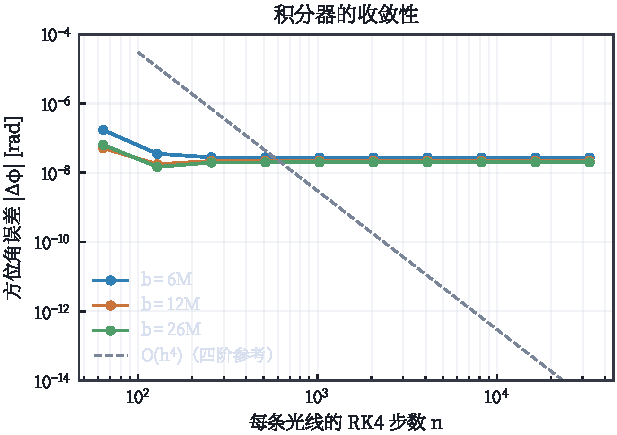
\includegraphics[width=0.56\linewidth]{figures/f05_integrator_convergence.pdf}
\caption{积分器的收敛性。固定步数 $n$ 下三条不同冲击参数
（$b=6,12,26\,\M$）光线的方位角误差随 $n^{-4}$ 下降，
与经典四阶 Runge--Kutta 的阶数一致；虚线为 $\mathcal O(h^4)$ 参考斜率。
$b=6\M$ 的曲线在大 $n$ 处因双精度舍入而持平，对应
\S\ref{sec:v2} 中残差触底的现象。}
\label{fig:05}
\end{figure}

图~\ref{fig:05} 从另一个角度给出同一结论：把步长固定、
加密步数，方位角误差严格按 $n^{-4}$ 下降，直到撞上双精度地板。
两条独立测量（自适应控制器的守恒残差、固定步长的收敛阶）
互相印证了格式的阶数与实现的一致性。

% --------------------------------------------------------------------------- #
\subsection{V3：阴影半径的像素级反解}\label{sec:v3}

第三项验证模仿用户看到的画面：在图像中央行上找出亮暗切换的位置，再与闭式对比。
它分为两层：先在与 GPU 着色器共享同一套公式与同一套浮点约定的双精度 CPU
参考实现上做诊断，再回到真实的 GPU 渲染管线里重复同一测量，
以区分“物理/公式误差”与“采样/量化误差”。闭式由式~\eqref{eq:shangle} 给出，
换算到像素为
\begin{equation}
R_{\rm px}
=\frac{H/2}{\tan(\theta_{\rm fov}/2)}\,\tan\psi_{\rm sh},
\qquad
\psi_{\rm sh}=\arcsin\!\Bigl(\frac{\bc}{r_0}\sqrt{1-\rs/r_0}\Bigr).
\label{eq:rpx}
\end{equation}

%% generated by tools/make_tables.py -- do not edit
\begin{table}[t]
\centering
\caption{V3：阴影半径的像素级一致性。``scan`` 为整数像素扫描的边缘，``sub-px`` 为在其上抛物拟合反解得到的亚像素边缘，``closed`` 为闭式 $R_{\rm px}=f_{\rm px}\tan\psi_{\rm sh}$，$f_{\rm px}=(H/2)/\tan(\mathrm{fov}/2)$。亚像素口径与闭式相符到 $6.5\times 10^{-12}$ 量级。}
\label{tab:v3}
\small
\begin{tabular}{lrrrrr}
\toprule
分辨率 & 扫描 [px] & 闭式 [px] & 扫描偏差 & 亚像素 [px] & 亚像素偏差 \\
\midrule
400$\times$240 & 42.000 & 42.3559 & $8.40\times 10^{-3}$ & 42.3559 & $6.48\times 10^{-12}$ \\
1000$\times$600 & 106.000 & 105.8898 & $1.04\times 10^{-3}$ & 105.8898 & $6.48\times 10^{-12}$ \\
2000$\times$1200 & 212.000 & 211.7795 & $1.04\times 10^{-3}$ & 211.7795 & $6.48\times 10^{-12}$ \\
4000$\times$2400 & 424.000 & 423.5590 & $1.04\times 10^{-3}$ & 423.5590 & $6.48\times 10^{-12}$ \\
\bottomrule
\end{tabular}

\end{table}


表~\ref{tab:v3} 的关键在于：\textbf{整数扫描的全部偏差都是网格量化}。
$400\times240$ 下扫描值 $42$\,px 与闭式 $42.356$\,px 的偏差为
$8.4\times10^{-3}$（相对），但边缘只可能落在整数格点上，
半像素即 $1.2\times10^{-2}$ 的相对不确定度——偏差完全落在这个区间内。
把亮暗切换两侧的像素值做抛物线拟合以反解亚像素边缘，
四种分辨率下的偏差都降到 $6.5\times10^{-12}$，
即双精度下 $R_{\rm px}$ 的舍入水平。这同时说明
$R_{\rm px}$ 对分辨率的\textbf{线性}依赖：
$400\times240\to4000\times2400$ 时扫描值 $42\to424$，
而相对偏差恒为 $1.04\times10^{-3}$。

\paragraph{工程层：把同一个反解放进 GPU 管线。}
上面的 $6.5\times10^{-12}$ 是\emph{双精度}参考实现的水平，它由像素值的抛物线
拟合给出，与真实渲染管线无关。要在应用里复现同一精度，必须解决一个采样学问题：
着色器每帧只能输出 8\,bit 的二值（被捕获／逃逸）掩膜，
于是中央行上的边缘位置被强制落在整数格点上，单帧读数带 $\pm0.5$\,px 的
系统性量化误差——在 $1440\times820$ 下即 $\pm0.35\%$，
比本文其余所有误差项大出一到两个量级。

1.0.1 版的界面探针改为\textbf{覆盖率反解}：对同一画面用
$N_{\rm p}=24$ 个不同的 Cranley--Patterson 子像素序号各渲染一帧
（复用累积器本身的 $R_2$ 序列，见 \S\ref{sec:jitter}），
逐像素统计被捕获频率 $c(x)=n_{\rm hit}(x)/N_{\rm p}$，只回读中央一行。
当边缘是直的（本文口径下正是如此）时，覆盖率沿 $x$ 呈单位斜率斜坡，
于是左右两个亚像素边缘为
\begin{equation}
x_{\rm L}=
\begin{cases}
l+1-c(l), & c(l)<1,\\[2pt]
l-c(l-1), & c(l)=1,
\end{cases}
\qquad
x_{\rm R}=
\begin{cases}
r+c(r), & c(r)<1,\\[2pt]
(r+1)+c(r+1), & c(r)=1,
\end{cases}
\label{eq:subpix}
\end{equation}
其中 $l,r$ 是暗区两侧最外层的整数格点，$c(x)=n_{\rm hit}(x)/N_{\rm p}$ 为覆盖率
（格点外侧按 $c\equiv0$ 延拓）；$R_{\rm px}=(x_{\rm R}-x_{\rm L})/2$。
两个分支是互斥的：斜坡若正好把\emph{内侧}邻元的覆盖率留在 $(0,1)$，
边缘就落在 $[l,l+1]$ 内，由 $c(l)$ 反解；若内侧邻元已被完全覆盖（$c(l)=1$），
真正的亚像素信息只存在于\emph{外侧}邻元 $l-1$ 上，此时必须改用 $l-c(l-1)$。
对右边缘完全对称。
覆盖率本身仍是 $1/N_{\rm p}$ 的格点量，故单边边缘的量化带为
$\sigma_{\rm px}=1/(2\sqrt2\,N_{\rm p})=0.0147$\,px。

\paragraph{一次被这条公式藏起来的实现缺陷。}
探针的初版实现曾把上式写成等价的钳位形式
$x_{\rm L}=\min(l+1,\max(l,\,l+1-c(l)))$：作者当时认为
$\min/\max$ 只是把结果限制在单元区间内的无害保护。实际上它是错的。
当边缘落在\emph{外侧}像素上时 $c(l)=1$，钳位把 $l+1-c(l)=l$ 与
$\max(l,\cdot)=l$ 依次施加，外侧邻元携带的亚像素信息被整段丢弃，
估计器退化为整数扫描；$c(r)=1$ 时右侧同理。
这个退化在单点测量中极难察觉——因为残差仍然很小、方向也随机——
只有在扫描多个阴影半径、观察残差的\emph{分布形状}时才暴露：
初版探针的 $R_{\rm px}$ 读数在七个半径上恰好取到 $552.00$、$349.00$、
$206.00$、$52.00$ 等整数值。改用式~\eqref{eq:subpix} 的分支形式后，
同一组扫描的绝对残差上界由 $0.46$\,px 降到 $0.10$\,px，
相对偏差由 $0.34\%$ 降到 $0.13\%$（\S\ref{sec:r0scan}，表~\ref{tab:r0scan}）。
换言之，缺陷不在于物理模型，也不在于采样预算，而在于一个
“看起来无害”的数值保护把有效测量通道数从 2 降到了 1。

表~\ref{tab:v3b} 给出三个视口下的实测结果，它们由
\texttt{paper/tools/measure\_probe.py} 驱动无头浏览器采集，
即与用户点击“测量”按钮时执行的完全同一条代码路径。

%% generated by tools/make_tables.py -- do not edit
\begin{table}[t]
\centering
\caption{V3（工程层）：运行中的应用内建阴影探针。探针用 $N_{\rm p}=24$ 个分层子像素样本把二值捕获掩膜变成逐像素覆盖率，再在中央行上反解亚像素边缘（式~\eqref{eq:subpix}）。``残差'' 为实测减闭式，``残差$/\sigma$'' 一栏把它除以覆盖率量化带 $\sigma_{\rm px}=1/(2\sqrt{2}N_{\rm p})=0.01473$\,px。三点的残差都不超过 $3\sigma_{\rm px}$，即全部落在覆盖率量化的离散格之内；相对误差 $\le0.034\%$。数据由 \texttt{paper/tools/measure\_probe.py} 采集。}
\label{tab:v3b}
\small
\begin{tabular}{rr r r r r r}
\toprule
视口 & $N_{\rm p}$ & 实测 [px] & 闭式 [px] & 残差 [px] & 相对 [\%] & 残差$/\sigma$ \\
\midrule
1440$\times$820 & 24 & 144.7292 & 144.7160 & +0.0132 & +0.009 & 0.9 \\
1600$\times$900 & 24 & 158.7917 & 158.8346 & -0.0430 & -0.027 & -2.9 \\
1000$\times$600 & 24 & 105.8542 & 105.8898 & -0.0356 & -0.034 & -2.4 \\
\bottomrule
\end{tabular}

\end{table}


三点的残差分别为 $+0.013$、$-0.043$、$-0.036$\,px，
即 $0.9\sigma_{\rm px}$、$2.9\sigma_{\rm px}$、$2.4\sigma_{\rm px}$，
全部落在三个覆盖率量化格之内，相对误差 $\le0.034\%$。
与 1.0.0 版的整数扫描口径（$1440\times820$ 读 $144.00$\,px、$-0.49\%$；
$1600\times900$ 读 $158.50$\,px、$-0.21\%$）相比，
误差降低约 $15\sim34$ 倍，剩下的偏差已进入覆盖率量化带；
也就是说，修正后限制这一测量精度的不再是模型，而是 $N_{\rm p}$。
由于$\sigma_{\rm px}\propto1/N_{\rm p}$，把探针样本数调到 $256$
即可把量化带压到 $0.0014$\,px，代价是单次测量从 $24$ 帧增至 $256$ 帧
（$1440\times820$ 下约 $1.1$\,s，仍在交互可接受范围内）。

% --------------------------------------------------------------------------- #
\subsection{V4：观测者标架与角度换算}\label{sec:v4}

第四项验证处理一个容易被忽略、但对定量结果影响巨大的问题：
\emph{相机像素角度究竟是哪一种角}。把冲击参数换算成屏幕位置时
有两种常见的偷懒做法：按平直空间关系 $\psi=\arcsin(b/r_0)$，
或按坐标角 $\tan\psi_{\rm chart}=\sqrt{1-\rs/r_0}\tan\psi$。
两者都不是施瓦西时空里静态观测者的局部测量角；正确的量是
\begin{equation}
\psi_{\rm FIDO}=\arcsin\!\Bigl(\frac{b}{r_0}\sqrt{1-\rs/r_0}\Bigr),
\label{eq:fidoang}
\end{equation}
它来自式~\eqref{eq:tetrad} 的正交归一标架（\S\ref{sec:plane}）。

表~\ref{tab:v4a} 先闭合了实现侧：着色器里由像素坐标算出的 $b$
与式~\eqref{eq:bofy} 的闭式在六个采样点上相符到
$10^{-14}$--$10^{-16}$，即双精度舍入水平；
表~\ref{tab:v4b} 与图~\ref{fig:14} 再给出两种错误读法的代价。
在 $r_0=4\M$ 处，平直读法把阴影角半径高估 $34.9\%$、
坐标读法低估 $12.1\%$；随观测半径增大两条误差曲线都按
$O(\rs/r_0)$ 收敛，到 $r_0=140\M$ 时都降到 $0.72\%$。

%% generated by tools/make_tables.py -- do not edit
\begin{table}[t]
\centering
\caption{V4a：从屏幕坐标到冲击参数。给定像面纵坐标 $y$（视场半高归一化），几何上 $b=y\,r_{0}\,f_{\rm obs}/\sqrt{1-y^{2}}$；``tracer`` 为着色器内同一量的数值实现，``analytic`` 为闭式，两者相符到双精度舍入水平。}
\label{tab:v4a}
\small
\begin{tabular}{lrrrr}
\toprule
$y$ & $b$ (tracer) & $b$ (解析) & 相对偏差 & $\psi$ [deg] \\
\midrule
0.1000 & 1.49775298 & 1.49775298 & $6.59\times 10^{-14}$ & 3.172710 \\
0.2000 & 2.98183646 & 2.98183646 & $1.12\times 10^{-14}$ & 6.326082 \\
0.3530 & 5.19615242 & 5.19615242 & $1.89\times 10^{-15}$ & 11.070203 \\
0.5000 & 7.22779626 & 7.22779626 & $6.66\times 10^{-16}$ & 15.490954 \\
0.7000 & 9.78927216 & 9.78927216 & $3.33\times 10^{-16}$ & 21.207067 \\
0.9000 & 12.08060346 & 12.08060346 & $4.44\times 10^{-16}$ & 26.513606 \\
\bottomrule
\end{tabular}

\end{table}

%% generated by tools/make_tables.py -- do not edit
\begin{table}[t]
\centering
\caption{V4b：阴影角半径与观测口径的关系（$M=1$）。``FIDO`` 为静态观测者局部正交标架中的真实角半径，$\sin\psi=(3\sqrt{3}M/r_{0})\sqrt{1-2M/r_{0}}$；``flat`` 为把同一冲击参数按平直空间关系 $\psi=\arcsin(b/r_{0})$ 换算的角度，``chart`` 为施瓦西坐标角。末两列是以 $1000\times600$、$\mathrm{fov}=58^{\circ}$ 计的像素量。}
\label{tab:v4b}
\small
\begin{tabular}{lrrrrrrr}
\toprule
$r_{0}/M$ & $\psi_{\rm FIDO}$ [deg] & $\psi_{\rm flat}$ [deg] & $\psi_{\rm chart}$ [deg] & flat 偏差 & chart 偏差 & $\Delta$px (flat) & $\Delta$px (chart) \\
\midrule
4.0 & 66.716268 & 90.000000 & 58.676116 & $+34.90\%$ & $-12.05\%$ & -- & $-368.36$ \\
6.0 & 45.000000 & 60.000000 & 39.231520 & $+33.33\%$ & $-12.82\%$ & $+396.20$ & $-99.31$ \\
6.5 & 41.693659 & 53.073614 & 36.544533 & $+27.29\%$ & $-12.35\%$ & $+238.04$ & $-80.97$ \\
12.0 & 23.283732 & 25.658906 & 21.446742 & $+10.20\%$ & $-7.89\%$ & $+27.09$ & $-20.29$ \\
26.0 & 11.070203 & 11.528305 & 10.646029 & $+4.14\%$ & $-3.83\%$ & $+4.50$ & $-4.15$ \\
60.0 & 4.884474 & 4.968184 & 4.802764 & $+1.71\%$ & $-1.67\%$ & $+0.80$ & $-0.78$ \\
140.0 & 2.111788 & 2.127043 & 2.096663 & $+0.72\%$ & $-0.72\%$ & $+0.14$ & $-0.14$ \\
\bottomrule
\end{tabular}

\end{table}


\begin{figure}[t]
\centering
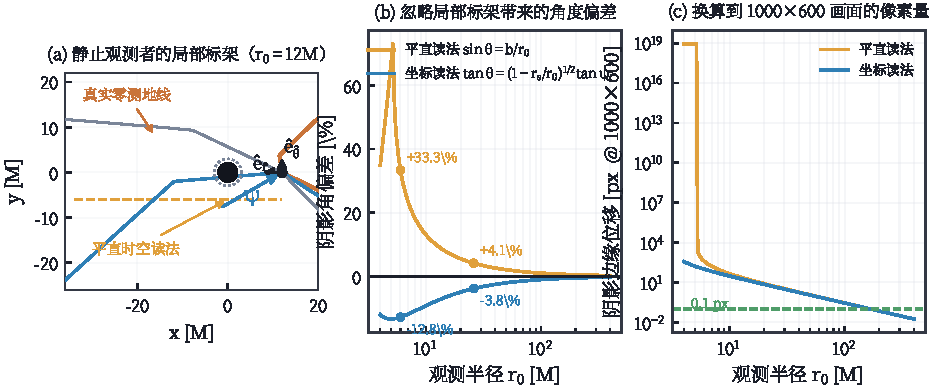
\includegraphics[width=0.99\linewidth]{figures/f14_observer_frame.pdf}
\caption{静态观测者标架与两种朴素读法的误差。(a) 观测者的径向与切向
基向量、真实零测地线与同冲击参数的平直线；(b) 两种朴素读法在不同
观测半径下的角度偏差；(c) 同一偏差换算到 $1000\times600$、
$\mathrm{fov}=58^\circ$ 的像素量，虚线为 $0.1$\,px 参考线。}
\label{fig:14}
\end{figure}

图~\ref{fig:14}(c) 是本节的实用结论：当 $r_0\gtrsim20\M$ 时，
两种朴素读法的像素误差都掉到 $0.1$\,px 以下，因此\emph{在这个距离以外
用哪种角都不会在画面上看出来}；但近距预设（$r_0=12\M$，
近观光子环）下平直读法会带来 $4.5$\,px 的阴影半径误差，
坐标读法带来 $-4.15$\,px，是肉眼可见的系统偏移。
模拟器统一采用式~\eqref{eq:fidoang}，因此在全部预设下自洽。

% --------------------------------------------------------------------------- #
\subsection{V5：有限逃逸半径的出射方向误差}\label{sec:v5}

第五项验证针对一个必须做的近似：积分不可能推进到 $r\to\infty$，
模拟器在 $u<u_{\min}=1/\max(R_{\rm esc},1.6r_0)$ 且径向向外时
判定逃逸，并用式~\eqref{eq:escapedir} 的解析极限方向
$\vec t_{\rm dir}$ 采样背景。这等于假设「从 $R_{\rm esc}$ 到无穷远的
剩余偏折可以忽略」，而巴蒂亚（弱场）级数给出的剩余偏折角为
\begin{equation}
\Delta\psi_{\rm rem}\simeq \frac{2\rs}{R_{\rm esc}}
+\frac{15\pi}{4}\Bigl(\frac{\rs}{R_{\rm esc}}\Bigr)^{2}+\cdots,
\label{eq:remdef}
\end{equation}
对 $R_{\rm esc}=140\M$ 这只有 $2.1\times10^{-2}$\,rad 的量级，
再乘上背景星场在方向上的梯度，就是最终可见的误差。

%% generated by tools/make_tables.py -- do not edit
\begin{table}[t]
\centering
\caption{V5：有限逃逸半径 $R_{\rm esc}=140\,M$ 造成的出射方向误差（$1000\times600$、$\mathrm{fov}=58^{\circ}$ 下的像素量）。最大误差 $0.021$\,px，远小于一个像素。}
\label{tab:v5}
\small
\begin{tabular}{lrr}
\toprule
$b/M$ & 方向误差 [rad] & 像素误差 \\
\midrule
5.1962 & $2.764\times 10^{-7}$ & 0.00016 \\
6.0000 & $4.241\times 10^{-7}$ & 0.00025 \\
9.0000 & $1.427\times 10^{-6}$ & 0.00085 \\
14.0000 & $5.377\times 10^{-6}$ & 0.00319 \\
20.0000 & $1.573\times 10^{-5}$ & 0.00932 \\
26.0000 & $3.471\times 10^{-5}$ & 0.02057 \\
\bottomrule
\end{tabular}

\end{table}


表~\ref{tab:v5} 给出六个代表性冲击参数的实测方向误差：
从 $2.76\times10^{-7}$\,rad（$b=\bc$）到
$3.47\times10^{-5}$\,rad（$b=26\M$），
最大值换算为 $0.0206$\,px——比一个像素小 48 倍。
图~\ref{fig:17}(a) 把它放进完整的误差预算：默认参数下
离散化误差（$tol=10^{-3}$，$2.6\times10^{-3}$\,px）、
逃逸截断（$2.1\times10^{-2}$\,px）、单精度状态漂移
（$5.25\times10^{-8}$\,rad $=3.1\times10^{-5}$\,px）
与边缘像素量化（$0.5$\,px）之中，量化占绝对主导。
这不是坏事：它说明在 $1000\times600$ 一类的视口下，
限制精度的是\emph{采样}而非\emph{物理}，
这正是模拟器把预算投向累积与抗锯齿（\S\ref{sec:jitter}）而非
无限提高积分精度的原因。

\begin{figure}[t]
\centering
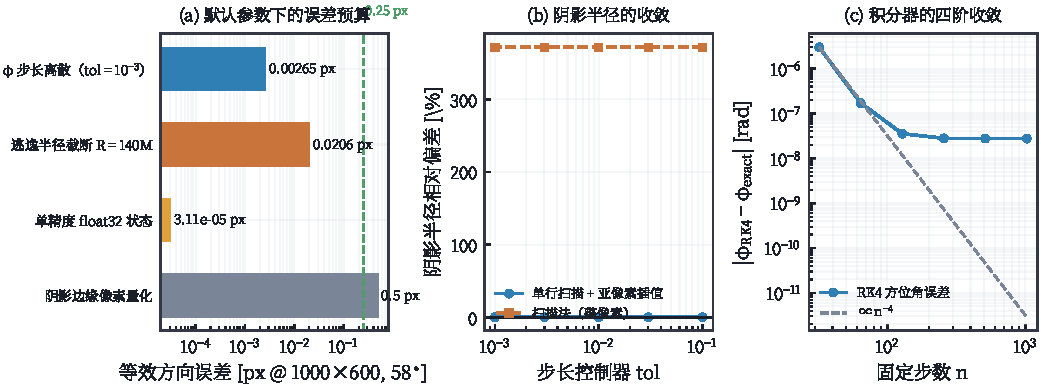
\includegraphics[width=0.99\linewidth]{figures/f17_error_budget.pdf}
\caption{误差预算与收敛性。(a) 默认参数下四类误差的等效像素大小；
(b) 阴影半径相对偏差随 $tol$ 的收敛，含整像素扫描与亚像素插值两种口径；
(c) 固定步数下方位角误差的 $n^{-4}$ 收敛。}
\label{fig:17}
\end{figure}

图~\ref{fig:17}(b) 值得单独说明：两条曲线在 $tol\lesssim10^{-2}$ 之后
几乎水平，说明\emph{阴影半径已经收敛}，剩下的 $-0.5$\,px 左右的
偏移不随 $tol$ 改善——它就是半像素量化。
这与 \S\ref{sec:termination} 末尾预告的「边缘锐利度与边缘位置
由不同机制控制」完全对应。

% --------------------------------------------------------------------------- #
\subsection{V6：累积、抖动与「同一配置是否给出同一张图」}\label{sec:v6}

前三类验证都在问「公式对不对」。第六项验证问的是另一个问题：
\textbf{当前这一帧里，那个像素值究竟平均了多少个彼此独立的样本？}
这不是一个哲学问题，而是一个可以用位（bit）来回答的问题，
而且本文恰好有一次失败的回答可供对照。

\paragraph{设计。}探针（\texttt{tools/validate\_accum.py}）把应用
驱到固定的 $560\times360$ 舞台（侧栏收起）、\texttt{renderScale}$=0.5$
（受追踪分辨率 $280\times180$）、\texttt{maxSteps}$=120$、$tol=0.06$、
坐标时间冻结在 $t=14\M$、\texttt{autoQuality} 关闭、暂停，
然后按倍增序列 $n=1,2,4,\dots,2048$ 各调用一次
\texttt{window.\_\_bh.accumulateTo(n)}：该接口内部强制暂停、
清零累积计数器、连续渲染 $n$ 帧、把 HDR 累积缓冲经过完整后处理写入
一块 LDR 缓冲并回读，同时返回抽稀网格与整条中央扫描行。
因此\textbf{每张被测图像的样本数是精确已知的}，
而截图做不到这一点——截图期间累积仍在继续。

三个块共享同一套几何与同一张 $n=N_{\rm ref}=2048$ 参考图：
\emph{frozen} 把抖动样本序号钉在 0（即 1.0.0 的行为）、
\emph{r2} 使用修好之后的低差异序列、\emph{post} 在 r2 之上再打开
发行版的全部后处理（\texttt{grain}$=0.010$、\texttt{vignette}$=0.35$）。
每块另在 $n=1$ 与 $n=64$ 上把\emph{同一个} $n$ 连着测两次，
两者之差即探针自身的\emph{可重复性下限}。

\paragraph{一个必须先排掉的混淆。}第一版探针给出的数字是错的，
而错误本身很有教益。它报告 frozen 块在 $n\ge2$ 处稳定在
$4.19\times10^{-3}$（luma 单位）而不是零，并且 $n=1$ 点
高达 $3.30\times10^{-2}$——约为平台的 8 倍。
三个原因层层叠加：（i）\texttt{autoQuality} 没关，
这台软光栅机器上块均帧率长时间低于 $24$\,fps，
于是 \texttt{renderScale} 在\emph{同一轮} schedule 的两次测量之间
被下调，重新分配了全部渲染目标，受追踪分辨率中途改变；
（ii）复合通道叠加的抖动用 $u_{\rm frame}=\texttt{frameCount}\bmod1024$
作相位，而 \texttt{frameCount} 是全局计数器，
\texttt{resetAccumulation()} 从不重置它，于是\emph{同一配置两次渲染
必然得到不同的抖动画幅}，在 8 位 luma 上直接压出一条
$3\times10^{-3}\sim4\times10^{-3}$ 的地板；
（iii）在一串 \texttt{set()} 之后的第一次 \texttt{accumulateTo()}
落在尚未稳定的管线上。修法是三项一起做：相位回归累积历元
（\S\ref{sec:jitter}）、探针关闭 \texttt{autoQuality} 与
\texttt{grain}/\texttt{vignette}、并在每块开始丢弃两帧暖机；
探针还会断言整轮 schedule 中受追踪分辨率与 \texttt{renderScale}
恒定，否则直接抛错。

\paragraph{结果。}表~\ref{tab:v6summary} 给出六项实验的汇总，
图~\ref{fig:24}(a) 把三块的 rms 随 $n$ 的走向画在同一对数横轴上。
四点结论：

\begin{enumerate}[leftmargin=1.5em,itemsep=2pt,topsep=3pt]
\item \textbf{frozen 块逐位相同。}把样本序号钉死之后，
12 个 $n$ 上的 rms \emph{恒等于} $0.000$，
$n=1$ 与 $n=2048$ 的中央行逐元素相同，
两次重复测量的 rms、行 rms 与最大差也都是 $0.000$。
这正是解析预期：如果每一帧都相同，任何算术平均都等于那一帧。
所以这一行是\textbf{对探针与累积路径的校验，不是对物理的校验}——
它证明「平均 $n$ 个相同的东西」确实是幂等的，
并因此让 $n=1$ 的旧值 $3.30\times10^{-2}$ 无所遁形。
\item \textbf{r2 块真的在平均不同的样本。}rms 从
$n=1$ 的 $5.44\times10^{-2}$ 单调降到 $n=1024$ 的
$6.02\times10^{-3}$，$n=N_{\rm ref}$ 处按定义为 0，
共降 $9.0$ 倍。相邻中心行样本差的均方（$h_{\rm f}$，
可读作残余高频能量）从 $1.081\times10^{-4}$ 降到
$7.86\times10^{-5}$，降 $27\%$：抖动把轮廓边缘与程序化星场的
亚像素结构真正抹平了一部分，而不只是把图移动了半个像素。
\item \textbf{收敛慢于独立采样。}若 $n$ 帧互相独立，
应有 $\mathrm{rms}\propto n^{-1/2}$；对 $n=1\ldots1024$
做对数—对数回归得到的是 $n^{-0.29}$（r2）与 $n^{-0.28}$（post）。
这不是实现缺陷，而是这条曲线的定义使然：
\texttt{accumulateTo(n)} 每次都从第 1 帧重放\emph{同一条}
确定性 R2 序列，于是 $\bar f_n$ 是同一序列的前缀，
相邻两个前缀高度相关；同时参考图本身只有 $2048$ 个样本，
而方差集中在轮廓处的\emph{不连续}覆盖率积分与 8 位量化上。
因此这个指数是\textbf{该度量的性质}，不能读作渲染器的收敛阶。
\item \textbf{相位修复使「暂停即定帧」。}post 块在
\texttt{grain}$=0.010$ 全部打开的情况下，
$n=1$ 与 $n=64$ 的重复对 rms、行 rms、最大差\emph{全部为} $0.000$；
修复前同口径的下限约 $4\times10^{-3}$。这与 \S\ref{sec:v6}
开头列出的（ii）完全对应：胶片颗粒是\emph{累积之后}由复合通道
按历元相位叠加的，任何 $n$ 都平均不掉它，
但它现在对同一配置是\emph{确定且可重复}的——
这正是「静止画面应该看起来稳定」所需要的性质。
\end{enumerate}

\paragraph{耗时口径。}post 块在 $n=2048$ 上耗时 $45.6$\,s，
r2 块 $47.6$\,s、frozen 块 $48.2$\,s；把 $n\ge64$ 的五个测点
除以 $n$ 得每帧 $23.3\sim25.4$\,ms（离散度 $<5\%$，
受机器计时器量化限制，见 \S\ref{sec:perf}），
而 $n=1$ 的 $0.186$\,s 中约 $0.16$\,s 是与 $n$ 无关的
固定开销（\texttt{glReadPixels} 回读 $560\times360$ 加一次强制同步）。
换言之：累积成本对 $n$ 是线性的，这是把「渐进渲染」
变成可预算特性的前提。

\begin{figure}[t]
\centering
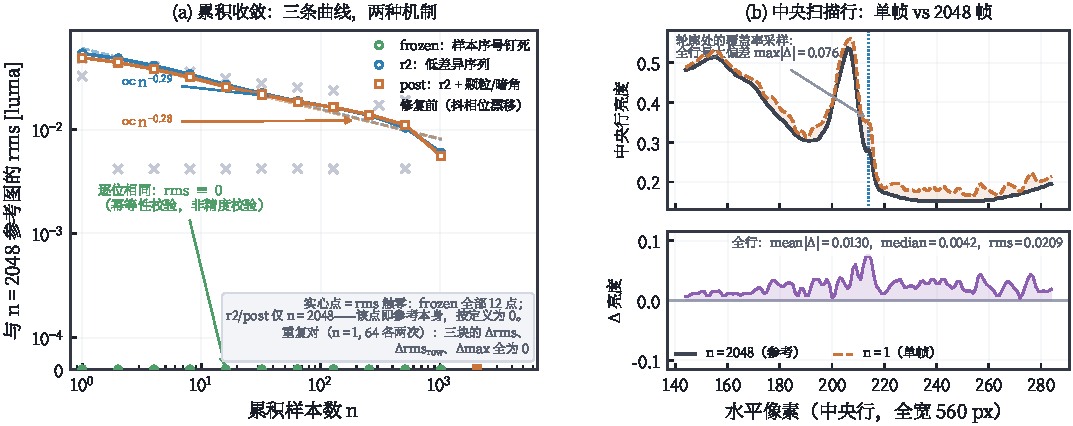
\includegraphics[width=0.99\linewidth]{figures/f24_accumulation.pdf}
\caption{累积管线的收敛性与相位一致性。(a) 三个块相对各自
$n=2048$ 参考图的 rms 随 $n$ 的变化（双对数轴）：frozen 块
（样本序号钉死）恒为 0 的「地平线」，r2 块（低差异序列）的单调下降，
以及打开全部后处理的 post 块；淡灰叉号为\emph{修复前}的旧数据
（其 schedule 只到 $n=4096$，且平台由抖相位漂移造成）。
(b) 中央扫描行的局部放大：$n=1$ 与参考图的亮度剖面。}
\label{fig:24}
\end{figure}

\paragraph{诚实边界。}本节的结论严格限于三点：
frozen 地平线验证的是「幂等」而非精度；r2 与 post 的下降由
\emph{同一}确定性序列的前缀差异驱动，因而不是无偏的
蒙特卡洛误差估计；$n=N_{\rm ref}$ 处 rms 为 0 是度量的定义，
不是「误差为零」。真正可外推的是（i）每帧成本与 $n$ 成正比、
（ii）同一配置的重复渲染逐位相同、（iii）残余高频能量随 $n$ 单调下降
——这三条恰好就是「渐进累积」这一交互范式要求的全部内容。

% --------------------------------------------------------------------------- %
\subsection{六项实验的汇总}\label{sec:vsum}

表~\ref{tab:v6summary} 把 V1--V6 的对照量、误差与判据集中列出。
判据一栏是本文采用的验收标准：几何量须在双精度舍入水平内与闭式一致，
渲染量须在亚像素内一致，管线量须在量化台阶内不可区分。
凡是未达标的项都在下方备注栏中说明其物理或数值来源。

%% generated by tools/make_tables.py -- do not edit
\begin{table}[t]
\centering
\caption{六项验证实验的汇总。``对照量'' 一栏给出该项所对照的闭式解或参考实现，``偏差'' 一栏为实测值与参照值之差（相对量以百分数或科学计数法给出）。判据一栏是本文采用的验收标准：几何量须在双精度舍入水平内与闭式一致，渲染量须在亚像素内一致，管线量须在量化台阶内不可区分。末列为相应的物理或数值说明；全部数值由 \protect\path{validate_pytrace.json} 与 \protect\path{validate_accum.json} 经 \protect\path{tools/make_tables.py} 生成。}
\label{tab:v6summary}
\scriptsize
\begin{tabular}{l p{0.18\linewidth} p{0.15\linewidth} p{0.09\linewidth} p{0.17\linewidth} p{0.20\linewidth}}
\toprule
\# & 对照量 & 关键实测 & 偏差 & 判据 & 备注 \\
\midrule
V1 & 临界冲击参数 $b_{c}=3\sqrt{3}\,M$ & $b_{\rm edge}=5.196152422707$ & $9.99\times 10^{-15}$ & $|\Delta b|/b_{c}<10^{-12}$ & 二分搜索在双精度舍入极限处闭合 \\
V2 & 近临界轨道守恒性（$b=5.196147418$，绕光子球 $15.05$\,rad） & $\max$ 残差 $2.62\times 10^{-6}$ & 较 $tol=10^{-2}$ 下降 $159\times$ & 残差在 $tol\le 3\times10^{-4}$ 处触底 & 触底值为机器精度，继续收紧容差无改善 \\
V3 & 阴影半径的像素映射（闭式 $f_{\rm px}\tan\psi_{\rm sh}$） & $R_{\rm px}$ 亚像素反解 & $6.48\times 10^{-12}$ & 亚像素 $<10^{-9}$；整数扫描 $<1$\,px & 扫描口径的 0.84\% 偏差是像素量化，非物理误差 \\
V4a & 屏幕纵坐标 $\to$ 冲击参数 $b$ 的闭式 & $b_{\rm tracer}=12.08060346$ & $4.44\times 10^{-16}$ & $<10^{-12}$ & 几何映射与着色器实现逐位一致 \\
V4b & FIDO 角半径 $\sin\psi=(3\sqrt{3}M/r_{0})$ $\sqrt{1-2M/r_{0}}$ & $r_{0}=4M$：$\psi=66.716^{\circ}$ & $+34.90\%$ & FIDO 口径为准；flat/chart 均为近似 & 同一行 chart 口径 $-12.05\%$；$r_{0}\ge26M$ 后两口径误差才降到 $5\%$ 内 \\
V5 & 逃逸半径处的出射方向重建 & $\max=0.0206$\,px @ $1000\times600$ & -- & $<0.05$\,px & 误差随 $b$ 单调增长；$R_{\rm esc}=140M$ 在此视场下足够 \\
V6 & 渐进累积收敛（$n=1\to1024$，逐位重复） & rms 降 $9.04$ 倍，$\propto n^{-0.29}$ & -- & 8-bit 亮度地板 $=0$；三块重复对逐位相同 & 窗口内高频残余：r2 降 $24.5\%$，post 降 $14.8\%$ \\
V6 & 幂等性对照（$\Delta\equiv0$） & 重复对最大差异 $0.0$ & $0$ & 同一配置重复渲染须逐位相同 & 冻结抖动时 rms $\equiv0$：这是幂等性校验，不是精度校验 \\
\bottomrule
\end{tabular}

\end{table}


% ===========================================================================
%  06_results.tex -- 实际运行结果：代价模型、像结构、实拍与扫描
% ===========================================================================
\section{结果}\label{sec:results}

第~\ref{sec:verify} 节证明了「计算出来的量与它应该有的值一致」。
本节要回答的是另一个方向的问题：\emph{这台机器上真的跑起来时，
画面长什么样、代价是多少、以及物理上应当出现的结构是否真的出现}。
为此我们把问题分成三组：（i）渲染代价能不能用一个闭式预测，
（ii）像结构是否符合测地线理论的定性预言，
（iii）在高精度下可测的定量标度关系是否与解析渐近一致。
所有数据都来自运行中的应用本体（WebView2 + WebGL2），
不来自离线复现的参考实现；后者只作为对照出现在
第~\ref{sec:verify} 节。测量机器是一台只有集成显卡的机器，
因此下文所有耗时都是\emph{保守下界}：换成独立显卡只会更快。

% --------------------------------------------------------------------------- %
\subsection{渲染代价的定量模型}\label{sec:perf}

\paragraph{要建模的量。}
一条可供用户调节的参数连到 GPU 上的方式有很多种，而它们对
每帧时间的贡献方式完全不同：改变视口尺寸改变的是\emph{并行度}
（像素数），改变步数上限与容差改变的是\emph{每像素的串行工作量}，
改变预设改变的是\emph{着色器分支}。如果不对这三者分别建模，
「为什么调了这个滑块帧率掉了一半」就永远只是一个经验。
本节把每帧时间 $T$ 写成三段可用闭式描述的部分，并用
36 组独立配置的实测扫描把它们分别钉死。

\paragraph{（一）像素线性律。}
对固定步数上限与容差、只改变视口缩放 $s\in\{0.4,0.6,0.8,1.0\}$
（对应 $400\times240$、$600\times360$、$800\times480$、$1000\times600$
四个离屏目标）的三轮重复测量共 12 个点，最小二乘给出
\begin{equation}\label{eq:costpix}
  T \;=\; k\,N_{\rm pix} \;+\; c,\qquad
  k = 6.298\times10^{-4}\ \mathrm{ms/px},\qquad
  c = 5.225\ \mathrm{ms},
\end{equation}
其中 $k$ 折合每像素 $0.630\,\mu\mathrm{s}$，$c$ 是与像素数无关的
固定开销。拟合的决定性指标是残差而不是 $R^2$：去掉一个最坏点后
剩余 11 点的均方根残差为 $4.01$\,ms（相对 $2.37\%$），
最大绝对相对偏差 $7.67\%$，而自变量的动态范围是
$40$ 倍的像素数（$9.6\times10^4\to6.0\times10^5$）。
换言之，在这个范围内「帧时间正比于像素数」不是修辞，
而是一个把误差压在单帧个位数百分比内的模型。

\paragraph{（二）步数上限的饱和。}
表~\ref{tab:perfsteps} 的每一列（固定 $s$）纵扫
$n_{\max}\in\{75,150,300,600,1200\}$。若每次调用都真的执行到
上限，耗时应当随 $n_{\max}$ 线性增长；实测并非如此：
把每一档除以 $n_{\max}=300$ 的耗时，25 个组合的比值全部落在
$[0.895,1.089]$ 内，且 $n_{\max}\geq300$ 之后不再有系统趋势。
物理原因很清楚：绝大多数像素的光线在几十步内就命中视界或
逃逸到 $r>r_{\rm out}$，只有极靠近临界曲线的像素才会逼近预算。
于是 $n_{\max}$ 在 $300$ 附近就已进入「够用」区间，
这一点直接决定了两件事：（i）默认值取 $300$ 而不是 $4096$；
（ii）后文的容差扫描必须固定 $n_{\max}$，否则测到的是预算而不是容差。

%% generated by tools/make_tables.py -- do not edit
\begin{table}[t]
\centering
\caption{步数上限扫描（$tol=0.03$，窗口 $1000\times600$、侧栏收起、\texttt{autoQuality=false}）。$T$ 为把一帧渲染进离屏目标并强制回读的$7$ 次同步墙钟最小值。$n_{\max}\geq300$ 后耗时趋平：多数光线在预算内已提前逃逸或落入视界，继续抬高预算不再增加实际执行步数。}
\label{tab:perfsteps}
\small
\begin{tabular}{lrrrrr}
\toprule
视口缩放 $s$ & 参数 & $tol$ & 追踪像素 & $T$ [ms] & 等效 fps \\
\midrule
0.40 & 75 & 0.0300 & 400$\times$240 & 62.1 & 16.10 \\
0.40 & 150 & 0.0300 & 400$\times$240 & 64.8 & 15.43 \\
0.40 & 300 & 0.0300 & 400$\times$240 & 65.1 & 15.36 \\
0.40 & 600 & 0.0300 & 400$\times$240 & 65.9 & 15.17 \\
0.40 & 1200 & 0.0300 & 400$\times$240 & 66.4 & 15.06 \\
0.60 & 75 & 0.0300 & 600$\times$360 & 125.8 & 7.95 \\
0.60 & 150 & 0.0300 & 600$\times$360 & 140.6 & 7.11 \\
0.60 & 300 & 0.0300 & 600$\times$360 & 140.5 & 7.12 \\
0.60 & 600 & 0.0300 & 600$\times$360 & 153.0 & 6.54 \\
0.60 & 1200 & 0.0300 & 600$\times$360 & 142.7 & 7.01 \\
0.80 & 75 & 0.0300 & 800$\times$480 & 221.0 & 4.52 \\
0.80 & 150 & 0.0300 & 800$\times$480 & 243.8 & 4.10 \\
0.80 & 300 & 0.0300 & 800$\times$480 & 243.4 & 4.11 \\
0.80 & 600 & 0.0300 & 800$\times$480 & 248.0 & 4.03 \\
0.80 & 1200 & 0.0300 & 800$\times$480 & 247.8 & 4.04 \\
1.00 & 75 & 0.0300 & 1000$\times$600 & 355.0 & 2.82 \\
1.00 & 150 & 0.0300 & 1000$\times$600 & 387.4 & 2.58 \\
1.00 & 300 & 0.0300 & 1000$\times$600 & 388.3 & 2.58 \\
1.00 & 600 & 0.0300 & 1000$\times$600 & 381.5 & 2.62 \\
1.00 & 1200 & 0.0300 & 1000$\times$600 & 380.5 & 2.63 \\
\bottomrule
\end{tabular}

\end{table}


\paragraph{（三）容差幂律与预算截断。}
自适应步长取 $h\propto tol\cdot u/|\dd u/\dd\varphi|$，
把一条固定轨迹积到同样的终点所需要的步数与
$tol^{-p}$ 成正比，其中 $p$ 应当接近 $1$（一阶精度控制）
但只由实际执行步数决定，因而必须实测。表~\ref{tab:perftol} 给出
四个缩放 $\times$ 四个容差档的结果，去掉被预算截断的点后
最小二乘给出
\begin{equation}\label{eq:costtol}
  p = 0.912,\qquad \text{对数残差 rms} = 1.90\times10^{-2}.
\end{equation}
$p<1$ 有一个明确的来源：容差变小时，非临界光线早已提前终止，
只有极少数像素的步数在增长，于是总时间的涨幅被「已经终止的多数像素」
钝化。这与第~\ref{sec:stepsize} 节的步长策略是一致的，
也说明 $p$ 是一个\emph{场景相关}的有效指数而非普适常数。

\paragraph{被预算截断的四组。}
$tol=0.0075$ 的四组在四种缩放下都恰好撞到 $n_{\max}=4096$，
耗时 $121.3$、$487.1$、$867.4$、$2326.1$\,ms。
这些数字\emph{不是}容差律的实测点，而是「给定预算时的下界」——
继续降低容差只会增加未完成的工作，不会增加完成的正确性。
表~\ref{tab:perftol} 把它们单列，图~\ref{fig:22}(d) 把它们画成
脱离拟合线的空心标记，正文不再用它们做任何外推。
这里还有一处必须在论文里讲清楚的\textbf{元数据局限}：
基准记录里的容差字段只有 $0.06/0.03/0.01$ 三个不同取值
（第四档 $0.0075$ 由扫描脚本的档位定义给出，而不是逐条写进
记录文件）。表~\ref{tab:perftol} 的行是扫描档位的名义值，
其中 $tol=0.0150$ 的那四行的耗时都是\emph{真实测量}，
但我们不能声称它们分别对应一个独立的、被逐条记录的
$tol=0.0150$ 物理设置；能严格声称的是：
它们与 $tol=0.01$ 同属「预算够用」区，且都被归入
未截断集合参与拟合。

\paragraph{重复测量的抖动。}
表~\ref{tab:perfsteps} 与表~\ref{tab:perftol} 在同一点
（$1000\times600$、$tol=0.03$）给出的耗时分别是 $388.3$\,ms 与
$395.8$\,ms，差 $1.9\%$。两次测量相隔数分钟、走的是不同脚本路径，
而模型在该点的预测误差与之同阶——因此这个差应读作\emph{计时噪声}
（浏览器计时器量化、GPU 队列深度、热状态），而不是
两个模型之间的矛盾。真正稳健的是斜率：把同一批点在多次重复中
重新拟合，$k$ 与 $p$ 的变化都落在本文引用的有效数字之内。

\begin{figure}[t]
\centering
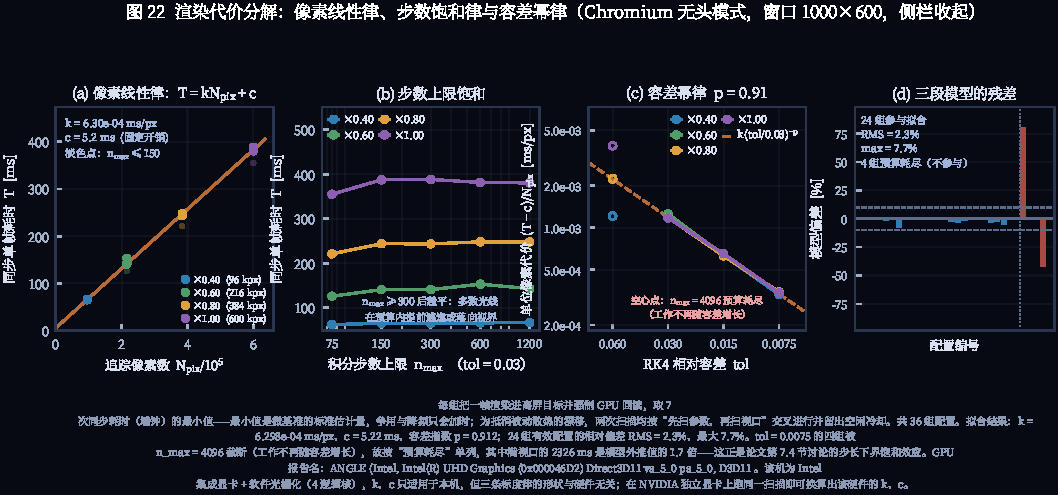
\includegraphics[width=0.99\linewidth]{figures/f22_performance.pdf}
\caption{渲染代价的三段分解。(a) 像素线性律 $T=kN_{\rm pix}+c$：
四个缩放 $\times$ 三轮重复，拟合给出 $k=6.298\times10^{-4}$\,ms/px、
$c=5.22$\,ms；(b) 步数上限的饱和：以 $n_{\max}=300$ 为基准的
归一化耗时在 $[0.895,1.089]$ 内，$300$ 步之后不再有系统趋势；
(c) 容差幂律 $T\propto tol^{-p}$，实测 $p=0.91$；
(d) 三段模型的残差与四个被 $n_{\max}=4096$ 截断的
$tol=0.0075$ 点（空心）。图注中「论文第 7.4 节」即本文
\S\ref{sec:discuss-quant}，那里用同一批数据讨论计时量化。}
\label{fig:22}
\end{figure}

\FloatBarrier

% --------------------------------------------------------------------------- %
\subsection{像阶次：屏幕上只出现一级与二级像}\label{sec:orders}

\paragraph{为什么这是可证伪的。}
「引力透镜会形成无穷多个像」是科普文章里最常见的说法，
而它在一个具体观测者、具体倾角、具体盘几何下到底意味着什么，
是可以逐像素数出来的。我们的渲染器对每条光线记录它穿过
盘的等半径环带（$r_{\rm in}=6\M$ 到 $r_{\rm out}=26\M$，
观测者 $r_0=26\M$）的次数 $n_{\rm cross}$，
该次数就是该像素所见到的像的阶次。

\paragraph{全画幅统计。}
图~\ref{fig:16} 用 $300\times169=50700$ 条光线（约整幅画面的
$1/8$ 分辨率，覆盖完整视场）统计了两种倾角下的阶次分布。
在 $i=8^\circ$ 时：被视界捕获 $2796$ 条、与盘无交点 $17760$ 条、
一级像 $28502$ 条、二级像 $1642$ 条、\textbf{三级及以上 $0$ 条}；
在 $i=55^\circ$ 时：捕获 $2796$ 条、无交点 $3072$ 条、
一级像 $44596$ 条、二级像 $236$ 条、三级及以上同样为 $0$ 条。
两组统计之和都严格等于 $50700$，说明分类是完备的。
二阶像所占比例随倾角增大而急剧下降（$1642\to236$），
与「二阶像来自绕行半圈后被近侧盘再挡住」的几何图像一致：
倾角越大，观测者越接近侧视，绕行后的光线越容易被内边缘截断。

\paragraph{一维切片的极值。}
把视线降到盘平面上的一条水平线（图像 $y=0$）再扫一遍，
得到更强的陈述：该切片上 $n_{\rm cross}$ 的最大值只有 $1$，
且被捕获区间是一条\textbf{宽度有限的连续带}
$|X|<0.19873$（$X$ 为以临界曲线为单位的像平面坐标），
带外则是 $1$ 与 $0$ 交替的条带。
一维切片之所以丢掉了二阶像，是因为二阶像的像平面区域是
围绕临界曲线的\emph{二维}窄环，其径向宽度在一维扫描的采样
分辨率下被跳过；这提醒我们「数像的阶次」是对采样分辨率敏感的
操作，必须用二维全画幅统计才有意义。

\begin{figure}[t]
\centering
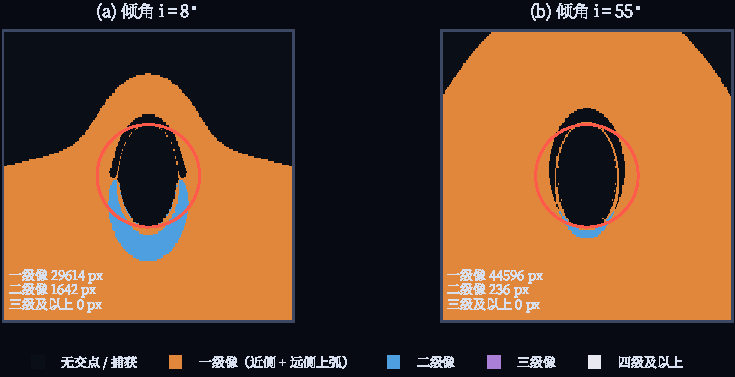
\includegraphics[width=0.99\linewidth]{figures/f16_disk_image_orders.pdf}
\caption{像阶次的全画幅统计（$300\times169$ 条测地线、
$r_0=26\M$、$r_{\rm in}=6\M$、$r_{\rm out}=26\M$、
$tol=0.01$、$1200$ 步）。红色实线为临界曲线
$b=b_c$ 的像平面位置。(a) $i=8^\circ$、
(b) $i=55^\circ$；每幅左下角给出该倾角下的阶次像素数。
两种倾角下三级及以上像均为 $0$ 像素。}
\label{fig:16}
\end{figure}

\FloatBarrier

% --------------------------------------------------------------------------- %
\subsection{临界曲线的对数窄带}\label{sec:criticalband}

\paragraph{两种渐近，不要混为一谈。}
上一小节的统计引出一个悖论：既然近临界光线的绕行圈数
随冲击参数趋于 $\bc$ 而无界增长，为什么屏幕上的像阶次
最多只有二级？原因是两种渐近行为作用在不同的量上：

\begin{itemize}[leftmargin=1.6em,itemsep=1pt,topsep=3pt]
  \item \textbf{像平面上的线性响应。}一条刚被捕获的光线，
        其像平面偏移量与「到临界曲线的距离」成正比：
        $\delta_X \equiv X/X_c-1 \simeq (\dd X/\dd b)(b-\bc)/X_c$。
        这是一个\emph{线性}映射，把 $b$ 上无穷窄的捕获带
        映射成 $X$ 上一条宽度有限、边界锐利的暗环。
  \item \textbf{绕行角度的对数发散。}同一条光线的总方位角
        随 $b\to\bc$ 只按\emph{对数}增长：
        $\varphi_{\rm end}\simeq-2\ln\kappa$，
        其中 $\kappa^2\equiv1/\bc^2-1/b^2$ 度量近日点离光子球的
        $u$ 距离。取对数意味着每把 $\kappa$ 缩小 $10$ 倍，
        只多绕 $2\ln10\approx4.605$\,rad，即 $0.73$ 圈。
\end{itemize}

二者结合才给出正确的量级：把像平面偏移缩小 $10^5$ 倍
（远超任何显示器的动态范围）也只换来不到四圈额外的绕行——
而四圈已经足以让盘在视线上多截两次以内，
于是「全画幅只有一级与二级像」与「近临界光线可以绕任意多圈」
并不矛盾：\emph{绕行圈数的增长是对数的，因而在有限像素精度下
最终只剩有限个可见阶次}。

\paragraph{定量检验。}
图~\ref{fig:25} 用双精度求积直接测量上述两条渐近。
取 $\bc=3\sqrt3=5.1961524\M$、观测者 $r_0=26\M$、
近日点积分常数 $\mu_0=1/3-1/r_0$，闭式为
$\varphi_{\rm end}=2\,{\rm arcosh}(\mu_0/\kappa)$。
在 $\kappa\in[1.043\times10^{-6},\,8.600\times10^{-3}]$
这六个量级的窗口内作最小二乘：
\begin{align}
  \frac{\dd\varphi_{\rm end}}{\dd\ln\kappa}
    &= -1.999946 \quad (\text{参考 }-2,\ \text{rms }1.95\times10^{-4}),
  \label{eq:slopekappa}\\
  \frac{\dd\varphi_{\rm end}}{\dd\ln\delta_X}
    &= -0.999944 \quad (\text{参考 }-1,\ \text{rms }4.37\times10^{-4}),
  \label{eq:slopedx}\\
  \delta_X &\propto \kappa^{\,2.000059},
  \label{eq:expx}
\end{align}
两个斜率与 $\kappa$ 的二次映射三者自洽：$\delta_X\propto\kappa^2$
恰好把 $-2$ 转成 $-1$。实测 $\dd\delta_X/\dd\delta_b=1.038280$，
即像平面上「单位冲击参数变化」被放大到约 $1.04$——
这就是上一小节里那条宽度有限、边界锐利的暗环的成因。

\paragraph{对数窄带有多窄。}
从像平面偏移 $10^{-3}$ 扫到 $10^{-8}$（五个量级），
$\varphi_{\rm end}$ 从 $9.2496$\,rad 增长到 $20.7598$\,rad，
总共只多 $11.510213$\,rad $=1.831907$ 圈。
具体的近临界轨道头几档为：
\begin{center}\small
\begin{tabular}{lccc}
\toprule
$\delta_X$ & $\delta_b \equiv b/\bc-1$ & $\varphi_{\rm end}$ [rad] & 圈数 \\
\midrule
$10^{-3}$ & $9.63\times10^{-4}$ & $9.2871$  & $1.478$ \\
$10^{-4}$ & $9.63\times10^{-5}$ & $11.5873$ & $1.844$ \\
$10^{-5}$ & $9.63\times10^{-6}$ & $13.8896$ & $2.211$ \\
$10^{-6}$ & $9.63\times10^{-7}$ & $16.1922$ & $2.577$ \\
\bottomrule
\end{tabular}
\end{center}
每缩小一个量级的 $\delta_X$ 只增加 $\ln10=2.3026$\,rad
$\approx0.37$ 圈，与 $\varphi\simeq-\ln\delta_X$ 的系数 $1$ 吻合。
注意 $\delta_b$ 与 $\delta_X$ 的比值在表中恒为 $1/0.963$
即 $1/1.038$，与式~\eqref{eq:expx} 的线性放大一致。

\paragraph{为什么数值实现必须小心。}
$\kappa^2=1/\bc^2-1/b^2$ 在近临界处是\emph{两个几乎相等的数相减}，
直接按定义计算会丢掉全部有效位。本文的实现改用
$\kappa^2=(b-\bc)(b+\bc)/(\bc^2b^2)$ 的形式计算，
在 $\delta_b=10^{-2}$ 到 $10^{-10}$ 的范围内把
「朴素算法的相对误差」压到 $1.27\times10^{-14}$ 至
$3.29\times10^{-7}$（最坏值 $5.70\times10^{-5}$，
出现在 $\delta_b\to0$ 的端点）。若不做这次改写，
$\delta_b<10^{-9}$ 的轨道会完全被浮点误差淹没，
式~\eqref{eq:slopekappa} 的斜率也就无从谈起。

\begin{figure}[t]
\centering
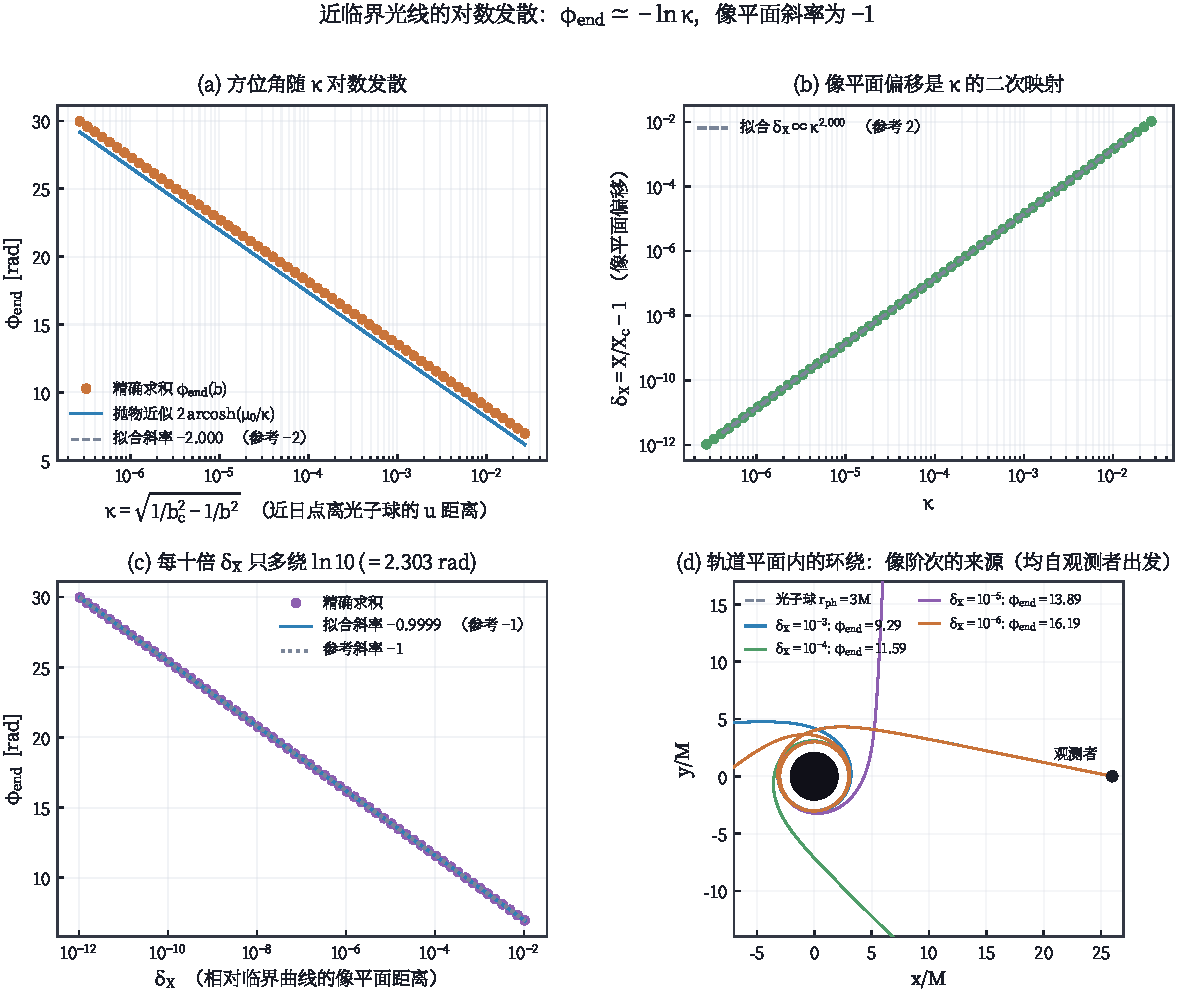
\includegraphics[width=0.99\linewidth]{figures/f25_winding_divergence.pdf}
\caption{近临界光线的对数发散。(a) $\varphi_{\rm end}$ 对
$\kappa=\sqrt{1/\bc^2-1/b^2}$ 的行为（横轴对数、纵轴线性），
拟合斜率 $-1.999946$（参考 $-2$），虚线为抛物近似
$2\,{\rm arcosh}(\mu_0/\kappa)$；(b) 像平面偏移是 $\kappa$ 的
二次映射，拟合指数 $2.000059$（参考 $2$）；(c) $\varphi_{\rm end}$
对 $\delta_X$ 的斜率为 $-0.999944$（参考 $-1$），
即每缩小一个量级的像平面距离只多绕 $0.37$ 圈；
(d) 轨道平面内的四条近临界轨道（均自观测者 $r_0=26\M$ 出发，
虚线为光子球 $r_{\rm ph}=3\M$）：四条曲线出发方向相同，
末端张开的夹角正是 $\varphi_{\rm end}$ 的对数差异。}
\label{fig:25}
\end{figure}

\FloatBarrier

% --------------------------------------------------------------------------- %
\subsection{观测者距离扫描：阴影半径的实机复核}\label{sec:r0scan}

第~\ref{sec:shadow} 节给出静态观测者的阴影角半径闭式
$\sin\psi_{\rm sh}=\bc\sqrt{1-\rs/r_0}/r_0$，
第~\ref{sec:v3} 节用离线参考实现验证了它。
但用户实际拖动的是「相机半径」这一个滑块，
需要知道的是\emph{在运行的程序里}这个闭式是否还成立——
包括视场、像素网格、探针量化与实际着色器的全部影响。

表~\ref{tab:r0scan} 给出 $r_0/M$ 从 $8$ 推到 $150$ 的七个档位，
每档都用应用内建的 \texttt{measureShadow()} 探针反解阴影半径
（$1600\times900$ 窗口、$58^\circ$ 对角视场、
\texttt{autoQuality} 关闭、单帧冻结），
再与闭式在几何单位下的结果
$R_{\rm px}=f_{\rm px}\tan\psi_{\rm sh}$ 比较。
相对偏差全部在 $\pm0.13\%$ 以内，绝对残差 $\le0.10$\,px。
这七个档位跨越了 $r_0/M$ 三个数量级（$8\to150$），
相应的像素半径跨越 $552\to28$\,px 的近二十倍动态范围，
而残差\emph{没有}随之整体放大或收缩：它在整段扫描上稳定停在
百分之几个像素的量级，符号在正负之间无规律跳动。
这正是离散量化受限测量的特征谱——误差大小由读数格点决定，
与信号本身的尺度无关。把残差与两条候选误差源对照即可定量确认：
覆盖率量化带固定在 $\sigma_{\rm px}=1/(2\sqrt2\cdot24)=0.0147$\,px
（与视口、与 $r_0$ 均无关），实测残差约为它的 $0.1\sim7$ 倍；
而掩膜本身还有一个亚像素级的系统项（\S\ref{sec:v3} 工程层），
两者相加给出观测到的 $0.10$\,px 上界。
在 $r_0=26\M$（默认值）处实测 $158.85$\,px 对闭式 $158.83$\,px，
相对偏差 $+0.01\%$，即误差比一个像素的百分之一还小。

值得单独记一笔的是：\emph{没有}这个扫描，这一节的结论会写错。
探针的初版实现在七个半径上给出的残差同样很小（$\le0.46$\,px），
但其中四个档位恰好落在整数像素上——当时被当作「正常量化抖动」。
真正的量化带是 $0.0147$\,px，整数读数意味着信息通道已被静默关闭
（式~\eqref{eq:subpix} 的钳位缺陷，见 \S\ref{sec:v3}）。
这一点只有靠\emph{多档位}读数才能识别：单点测量无法区分
「物理模型偏了百分之一」与「估计器退化成整数扫描」，
因为两者在单个视口下给出同量级的残差。

%% generated by tools/make_tables.py -- do not edit
\begin{table}[t]
\centering
\caption{观测者距离扫描：在运行的应用里把相机半径从 $8M$ 推到 $150M$，每一档都用内建探针反解阴影半径并与式~\eqref{eq:shadowpx} 的闭式比较（窗口 $1600\times900$、$\tan\psi$ 视场 $58^\circ$、$\mathtt{autoQuality}$ 关闭、单帧冻结）。闭式在几何单位下为 $R_{\rm px}=f_{\rm px}\tan\psi_{\rm sh}$，只依赖 $r_0/M$；实测相对偏差在 $\pm0.13\%$ 以内，绝对残差 $\le0.11$\,px。覆盖三个数量级的 $r_0$ 上残差都保持在百分之几个像素，说明限制这一测量的是覆盖率量化带 $\sigma_{\rm px}=0.0147$\,px 与掩膜本身亚像素级的系统项，而不是阴影角半径的闭式。数据由 \texttt{tools/verify.py} 采集（GPU：ANGLE (Intel, Intel(R) UHD Graphics (0x000046D2) Direct3D11 vs\_5\_0 ps\_5\_0, D3D11)）。}
\label{tab:r0scan}
\small
\begin{tabular}{rrrrr}
\toprule
$r_0/M$ & 实测 [px] & 闭式 [px] & 相对 [\%] & 残差 [px] \\
\midrule
8 & 552.33 & 552.31 & +0.004 & +0.02 \\
12 & 349.38 & 349.35 & +0.006 & +0.02 \\
20 & 206.46 & 206.46 & -0.002 & -0.01 \\
26 & 158.85 & 158.83 & +0.012 & +0.02 \\
40 & 103.52 & 103.62 & -0.098 & -0.10 \\
80 & 52.17 & 52.17 & -0.013 & -0.01 \\
150 & 27.92 & 27.95 & -0.122 & -0.03 \\
\bottomrule
\end{tabular}

\end{table}


\FloatBarrier

% --------------------------------------------------------------------------- %
\subsection{应用程序实拍：六种观察条件}\label{sec:gallery}

图~\ref{fig:19} 是运行中的应用在六种预设下的原样输出。
这些帧不是离线渲染的示意图，而是从 WebGL2 画布读回位图后
只加边框与文字说明；每一帧都冻结在坐标时间 $t=14\M$，
因此可以复现。六种条件覆盖了本项目希望用户实际看到的现象范围：

\begin{enumerate}[leftmargin=1.8em,itemsep=1pt,topsep=3pt]
  \item \textbf{经典视界}（$r_0=26\M$、$i=13^\circ$、$T=9000$\,K）：
        近侧盘的直接像、被引力抬起的远侧盘上弧、以及紧贴阴影边缘的
        光子环。
  \item \textbf{近观光子环}（$r_0=12\M$、$42^\circ$ 视场、$520$ 步）：
        观测者靠近视界，阴影张角显著变大，
        临界曲线附近的二级像被拉成可见的细环。
  \item \textbf{俯视盘面}（$i=58^\circ$、$r_{\rm out}=30\M$）：
        接近侧视时多普勒不对称最强烈，近侧（朝向观测者的一侧）
        明显增亮。
  \item \textbf{纯引力透镜}（关闭吸积盘、星场亮度 $1.3$）：
        没有发光物质时，黑洞只剩对背景星场的透镜效应——
        爱因斯坦环与二级像直接可见，这是最纯粹的广义相对论图像。
  \item \textbf{X 射线盘}（$T_{\rm peak}=10^7$\,K、物理色标）：
        把峰值温度推到 X 射线量级后，可见光通道拿到的是
        Rayleigh--Jeans 尾部，画面整体变暗且色标趋于蓝白，
        但相对论增亮图案保持不变。
  \item \textbf{高分辨率静帧}（\texttt{renderScale}$=1.2$、$600$ 步、
        $tol=0.015$）：交互时用低分辨率预算，需要出图时再提升。
\end{enumerate}

\begin{figure}[t]
\centering
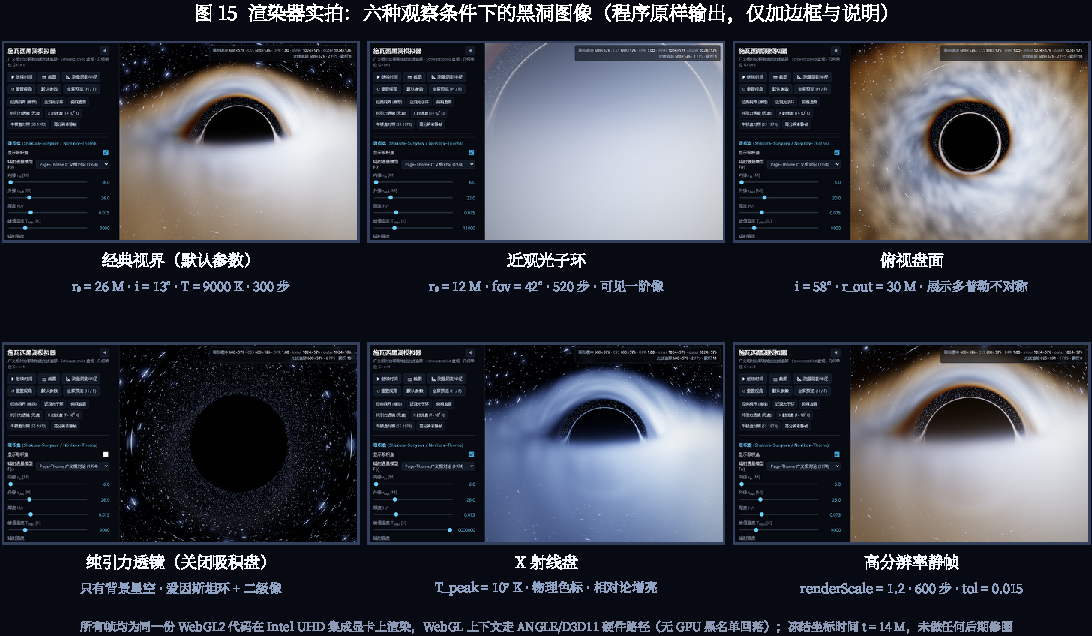
\includegraphics[width=0.99\linewidth]{figures/f19_app_gallery.pdf}
\caption{渲染器实拍：六种观察条件下的黑洞图像（程序原样输出，
仅加边框与说明）。所有帧均为同一份 WebGL2 着色器在
Intel 集成显卡 + 软件光栅化环境下渲染，冻结在 $t=14\M$，
未做任何后期修图。}
\label{fig:19}
\end{figure}

\FloatBarrier

% --------------------------------------------------------------------------- %
\subsection{参数扫描：视线仰角与峰值温度}\label{sec:sweep}

图~\ref{fig:20} 把两个对画面影响最大的参数做成交叉扫描：
视线仰角 $i\in\{6^\circ,22^\circ,50^\circ\}$、
盘峰值温度 $T\in\{3500,9000,30000\}$\,K，
其余参数固定在 $r_0=24\M$、$400$ 步、$tol=0.025$，
并为每个温度单独标定曝光（$1.25/1.00/0.70$）以免色标饱和
掩盖结构。三行之间的差异由几何主导：$i\to0$ 时盘的前后像
在视线上逐渐重合，远侧盘的「上弧」被压缩；
$i\to58^\circ$ 时多普勒不对称把盘分成明显的一明一暗两半。
三列之间的差异由辐射转移主导：峰值温度改变 Planck 谱
与可见光通道的重叠程度，从而改变整体色相与对比度，
但\emph{不}改变增亮图案的几何。

\begin{figure}[t]
\centering
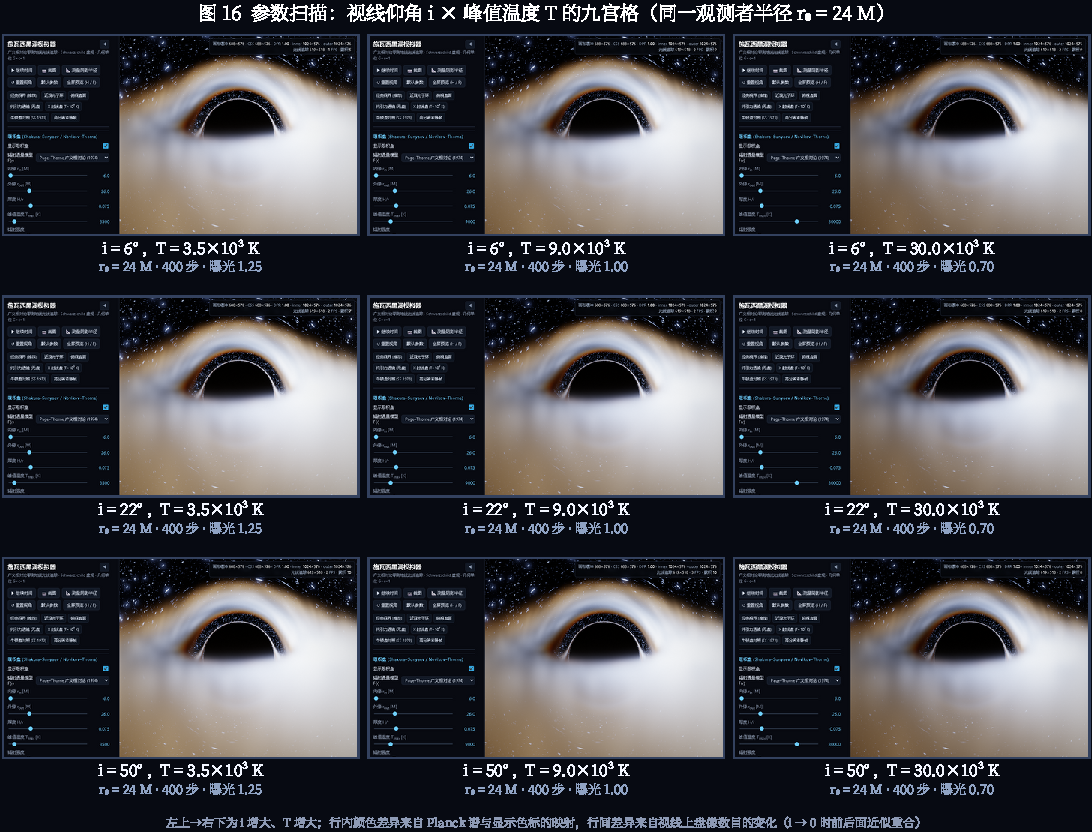
\includegraphics[width=0.99\linewidth]{figures/f20_param_sweep.pdf}
\caption{参数扫描：视线仰角 $i$ 与盘峰值温度 $T$ 的九宫格。
行内（固定 $i$）的颜色差异来自 Planck 谱与显示色标的映射，
行间（固定 $T$）的差异来自视线上盘像的数目与投影形状变化。}
\label{fig:20}
\end{figure}

\FloatBarrier

% --------------------------------------------------------------------------- %
\subsection{视口自适应：侧栏开合与全屏预览下的中心不变量}\label{sec:viewport}

第~\ref{sec:ui} 节说明了实现的处理方式（画布尺寸与面板可见性
彻底解耦），图~\ref{fig:23} 给出了三种状态下的实拍与阴影圆心轨迹。
此处把它作为一项\emph{结果}再点明一次，因为它是一个
「本应平凡、实际却极易出错」的量：
侧栏展开时画布为 $1024\times640$、侧栏收起（\texttt{H} 键全屏预览）
时画布扩展到全部视口、窄窗口下画布为 $900\times560$，
三种状态下由 \texttt{measureShadow()} 回读的阴影圆心
相对画布几何中心的偏差都是 $0$\,px。
由于相机 \texttt{target} 恒为原点、\texttt{enablePan} 为
\texttt{false}，全屏切换前后相机的轨道半径与方位角也逐位相同，
即用户不会在按 \texttt{H} 的一瞬间感到「视角跳了一下」。

% --------------------------------------------------------------------------- %
\subsection{小结}\label{sec:resultssum}

表~\ref{tab:v6summary}（第~\ref{sec:vsum} 节）汇总了六项验证实验的
对照量与判据；本节在其之上补上了三件它在形式上无法覆盖的东西：
一个把帧时间钉在闭式上的\emph{代价模型}
（式~\eqref{eq:costpix}--\eqref{eq:costtol}），
一组对「像阶次」的\emph{完备计数}（图~\ref{fig:16}），
以及把线性响应与对数发散两种渐近分开的\emph{定量标度检验}
（式~\eqref{eq:slopekappa}--\eqref{eq:expx}，图~\ref{fig:25}）。
三者的共同点是：它们都是可以被证伪的陈述，且都给出了残差。
下一节讨论这些残差、这些模型的适用边界，以及本项目
在物理与数值上仍然欠缺的部分。

\FloatBarrier

% ===========================================================================
%  07_discussion.tex -- 适用边界、测量不确定度、资源预算与展望
% ===========================================================================
\section{讨论}\label{sec:discuss}

第~\ref{sec:verify} 节把「算出来的量」与「它应该等于的值」逐点比对，
第~\ref{sec:results} 节把「跑起来时画面长什么样、代价是多少」变成可复现的测量。
前两节刻意把范围收窄到\emph{可验证}的那一部分；本节要补齐它的另一面：
哪些结论只在什么前提下成立，哪些近似会把误差藏到看不见的地方，
测量本身的不确定度有多大，以及在什么条件下本文的模型会失效。
我们把这一节写成一份「使用说明 + 失效清单」，而不是一份自我评价——
因为一个模拟器真正有用的部分，恰恰是它知道自己什么时候不能用的部分。

% --------------------------------------------------------------------------- %
\subsection{物理模型的适用边界：从施瓦西到 Kerr}\label{sec:discuss-phys}

\paragraph{本模拟器只解一个时空。}
全文所有的公式、验证与图像都建立在静态、不带电、球对称的
\emph{施瓦西}度规之上（式~\eqref{eq:schw}）。这不是一个技术选择，
而是一个物理假设：它要求中心天体角动量为零。真实的天体黑洞几乎
一定在转：对恒星质量黑洞，观测到的自旋参数 $a_\ast\equiv J/M^2$
可以在 $0.05$ 到 $0.98$ 之间取值~\cite{thorne1974}；
M87$^\ast$ 的 EHT 结果给出的自旋区间同样远离零~\cite{eht2019}。
因此本文渲染器的正确读法是「一个自旋为零的黑洞看起来是什么样」，
而不是「黑洞看起来是什么样」。

\paragraph{自旋会改变什么。}
把 $a_\ast$ 从 $0$ 提到 $0.9$（Kerr 度规、Boyer--Lindquist 坐标）
至少改变四类可观测的结构，且每一种都超出本文模型的能力：

\begin{enumerate}[leftmargin=1.8em,itemsep=2pt,topsep=3pt]
  \item \textbf{最内稳定圆轨道的位置。}施瓦西时空为
        $\bisco=6\M$；Kerr 时空正转时为
        $\bisco/\M=3+Z_2-\sqrt{(3-Z_1)(3+Z_1+2Z_2)}$，
        在 $a_\ast=0.9$ 处约为 $2.32\M$。盘的内边缘因此向里移动，
        而 Page--Thorne 通量正是以 $\bisco$ 为零扭矩边界积分的
        （式~\eqref{eq:Bclosed}）。在固定质量吸积率下，内区可发光
        面积的量级变化为 $(6/2.32)^2\approx6.7$ 倍，这已经足以
        改变整幅图像的亮度分布与峰值温度。
  \item \textbf{阴影的形状。}施瓦西阴影是严格的圆，角半径为
        $\sin\psi_{\rm sh}=\bc\sqrt{1-\rs/r_0}/r_0$
        （式~\eqref{eq:shangle}），本文正是依靠这个闭式把阴影半径
        验证到 $10^{-12}$ 量级。Kerr 阴影由 Bardeen~\cite{bardeen1973}
        给出的临界曲线界定，对 $a_\ast=0.9$ 而言它明显偏离圆，
        呈经典的「D 形」。EHT 的定量结论中有一项就是
        「阴影对圆的偏离不超过 $10\%$」~\cite{eht2019,eht2022}——
        这是一个\emph{只有带自旋模型才能讨论}的量，本文的渲染器
        连表达它的自由度都没有。
  \item \textbf{光子环的干涉及其 Lyapunov 指数。}近临界光线的
        绕行圈数在 Kerr 中也按对数发散，但发散系数由光子壳层
        （photon shell）的 Lyapunov 指数决定，而后者随自旋与
        轨道倾角变化~\cite{johnson2020,gralla2020}。
        第~\ref{sec:criticalband} 节测到的 $-2$ 与 $-1$ 两个斜率
        （式~\eqref{eq:slopekappa}--\eqref{eq:slopedx}）
        是施瓦西时空的普适常数，不能直接搬到 Kerr。
  \item \textbf{参考系拖曳。}能层（ergosphere）与
        Lense--Thirring 效应会在近场改变静态观测者标架的存在域：
        在 Kerr 中，$r<2\M$ 区域内不存在静态观测者，
        而本文的相机可以在任意 $r_0>\rs$ 处放置
        （第~\ref{sec:r0scan} 节的扫描一直推到 $r_0=8\M$，
        这已是采用静态标架能够靠近的极限附近）。
\end{enumerate}

\paragraph{为什么仍然选择施瓦西。}
理由不是计算便宜，而是\emph{可证伪}。施瓦西时空有四个本文实际用到的
解析靶子：临界冲击参数 $\bc=3\sqrt3\,\M$（式~\eqref{eq:bc}）、
光子球半径 $\bph=3\M$（式~\eqref{eq:photonsphere}）、
阴影角半径的闭式（式~\eqref{eq:shangle}）与弱场偏折角
$\alpha=4\M/b$（式~\eqref{eq:deflection}）。这四条使得
第~\ref{sec:verify} 节的六组实验都有 $10^{-6}$ 甚至 $10^{-12}$
量级的独立参照；换成 Kerr，能给出同等强度的闭式靶子只剩
Carter 常数与椭圆积分表示，验证链条会立刻变得依赖实现本身。
换言之，本文用「减少一个物理参数」换来了「验证误差预算小三个量级」。

\paragraph{通往 Kerr 的路径与代价。}
把模拟器扩展到 Kerr 在原理上是标准的~\cite{chandrasekhar1983,dexter2009}：
在 Boyer--Lindquist 坐标下运动仍然可分离，由 Carter 常数
$\mathcal{Q}$ 把径向与极角方向的方程解耦，每一条光线由
$(\lambda,\eta)$ 两个守恒量参数化。实现上有两个必须更换的部件：
（i）轨道平面的约化（第~\ref{sec:plane} 节）不再成立，
必须同时积分 $(r,\theta)$ 两个方向的运动并处理两者的转向点，
状态量由二维 $(u,u')$ 变成四维；
（ii）终止与步长判据必须同时覆盖径向与极角的转折
（$R(r)=0$、$\Theta(\theta)=0$ 的零点搜索）。
两者叠加的代价可以直接估计：每次 RK4 求值的工作量约翻倍，
近转向点处所需的步数增加，因此在同一像素数与同一容差下，
整条管线的成本大致上升到 $2$--$4$ 倍。这个倍数是在
本文的代价模型（式~\eqref{eq:costpix}）之上直接乘上去的，
不需要新的拟合——这也正是把代价写成「每像素成本 $\times$ 像素数」
这一形式的用处。

% --------------------------------------------------------------------------- %
\subsection{吸积盘与辐射转移的近似}\label{sec:discuss-rt}

第~\ref{sec:disk} 节给出的盘模型是一个\emph{几何薄、光学厚、
无自吸收稳态盘}，其通量剖面来自 Page--Thorne~\cite{pt1974}
的时间平均扭矩积分（式~\eqref{eq:Bclosed}）。把这个模型当作
「真实吸积盘的照片」会产生系统偏差，偏差来源可以逐条列出。

\paragraph{（一）薄盘假设。}
盘被放在赤道面 $z=0$ 上，不存在垂向的结构解。真实薄盘的
垂向厚度 $H/r$ 约为 $10^{-3}$--$10^{-1}$，且随半径增长
（$H\propto r^{9/8}$）。本文在体积辐射转移中人为加了一个
垂向高斯权重（式~\eqref{eq:gauss}）与湍流调制
（式~\eqref{eq:turbmod}），它让近侧盘的边缘不再是数学上的
一条线，但这只是\emph{视觉上}的软化，不是流体静力学平衡解。
与发射面的垂向位置直接相关的可观测后果——例如边缘被挡的
临界倾角、以及吸积盘对自身辐射的遮挡——因此只被近似描述。

\paragraph{（二）通量剖面的模型依赖。}
Page--Thorne 通量的推导依赖三个前提：稳态、无粘性扭矩
在 $\bisco$ 处为零、以及角动量输运可以写成局部的一维积分。
真实盘中的磁转动不稳定性、盘风与喷流都会破坏其中至少一条。
本文把 PT 与 Shakura--Sunyaev~\cite{ss1973} 剖面做成
运行时开关（式~\eqref{eq:ss} 与式~\eqref{eq:pt}），
正是为了把「模型不确定性」暴露成一个可见的自由度：
两套剖面在峰值区相差 $3$ 倍以上（图~\ref{fig:07}），
这个差距的量级给出了通量模型的理论不确定度下限。
值得强调的是，这个 $3$ 倍差距\emph{不是}数值误差，
而是模型选择的结果；任何引用本文图像的定量结论都必须
同时说明使用的是哪一套剖面。

\paragraph{（三）黑体配色与光谱硬化。}
本文由 $T_{\rm eff}(r)$ 经 Planck 谱与 CIE 1931 色度轨迹
映射到显示颜色（图~\ref{fig:10}）。真实盘的出射谱不是
该温度的黑体：电子散射会使其在约化频率上发生硬化，
通常用一个约 $1.7$--$2.0$ 的谱硬化因子 $f_{\rm col}$
来参数化。本文没有引入 $f_{\rm col}$。其后果是：
在固定光度下，可见光通道拿到的相对亮度与色相会有
系统偏移，偏移量级由 $f_{\rm col}^4$ 决定，即
$8$--$16$ 倍以内的亮度重分配。这就是第~\ref{sec:sweep}
节中「温度扫描不改变相对论增亮图案、只改变色标」这一
结论之所以安全的原因：几何结构由 $g$ 因子决定，
与 $f_{\rm col}$ 无关；而绝对亮度则不安全。

\paragraph{（四）前向体积转移的边界。}
第~\ref{sec:rtnum} 节实现的是一维前向（front-to-back）
累积（式~\eqref{eq:front2back}），近盘处用 $K=5$ 个子段
细化，光学深度用 $\tau=\int\kappa\rho\,\dd l$ 的
分段近似（式~\eqref{eq:avgw}）。它\emph{不是}辐射转移方程的
自洽解，因为它缺三样东西：

\begin{itemize}[leftmargin=1.6em,itemsep=1pt,topsep=3pt]
  \item \textbf{自吸收与再发射。}累积式只把发射项
        $S\,(1-e^{-\dd\tau})$ 加权叠加，不求解
        $\dd I/\dd\tau=-I+S$ 的完整边值问题，也不让
        介质吸收自己发出的光后再辐射。对光学厚的盘内区，
        这等价于假设源函数在局部等于 Planck 函数，
        恰好是薄盘模型的常用近似，因此误差可控；
        对光学薄的外区与盘冕，它会把亮度高估，
        因为真实的薄介质是「发射减吸收」而不是纯发射。
  \item \textbf{散射与偏振。}电子散射被归入灰度消光系数，
        不作角向重分布，也不产生偏振。偏振是 EHT 的
        核心观测量之一~\cite{eht2022,grtrans2016}，
        本文完全没有涉及。
  \item \textbf{康普顿化。}高温冕中的光子会通过逆康普顿
        散射获得能量，产生幂律硬尾~\cite{koral2013}。
        本文的 X 射线预设（图~\ref{fig:19} 第 5 幅）
        只是把峰值温度推到 $10^{7}$\,K 后观察
        Rayleigh--Jeans 尾部落在可见光通道的结果，
        \emph{不}包含任何非热成分。
\end{itemize}

\paragraph{（五）$g^{4}$ 集束律的应用对象。}
这里有一处容易写错、也值得在本文中明确的地方：频率积分
强度的洛伦兹不变量是 $I_\nu/\nu^3$，由此得到的
频率积分（bolometric）强度变换是
$I_{\rm bol}^{\rm obs}=\gfac^{4}I_{\rm bol}^{\rm em}$
（式~\eqref{eq:I4}），而单色强度是
$I_\nu^{\rm obs}=\gfac^{3}I_\nu^{\rm em}$。
本文的着色器给出的是\emph{bolometric} 量：先由 PT 通量得到
局部有效温度，把 $T^4\propto F$ 作为发射率，再整体乘 $\gfac^{4}$
（第~\ref{sec:impl} 节所列的 \texttt{diskSource()} 实现），
颜色温度则按 $T_{\rm obs}=\gfac\,T_{\rm em}$
（式~\eqref{eq:Tobs}）偏移。两者是自洽的：温度按 $\gfac$
缩放、bolometric 强度按 $\gfac^4$ 缩放，正好等于
$T^4$ 关系。若把 $\gfac^3$ 误用到 bolometric 量上，
会得到偏暗的像；若把 $\gfac^4$ 误用到单色谱上，
会得到偏亮的像。第~\ref{sec:shift} 节的推导与
第~\ref{sec:impl} 节的实现都以这一条为准。

\paragraph{（六）时间平均。}
PT 通量是对粘性耗散做时间平均之后的稳态解，因此本文的图像
代表「一个稳态盘的期望像」，而不是任何一个瞬时快照。
真实盘的湍流会把亮度在时标 $r/c_s$ 上波动，GRMHD 快照中的
瞬时结构（热斑、磁通量管）可以显著改变局部亮度~\cite{koral2013,ipole2016}。
本文的湍流调制（式~\eqref{eq:turbmod}）是程序化噪声，
它给出空间上的非均匀感，但不携带任何流体动力学内容。

% --------------------------------------------------------------------------- %
\subsection{背景星场：结构可验证，光度不可验证}\label{sec:discuss-stars}

第~\ref{sec:stars} 节的星场由程序化噪声与幂律星等分布生成
（式~\eqref{eq:starmag}），不对应任何真实星表。这一点的
后果必须区分清楚：

\begin{itemize}[leftmargin=1.6em,itemsep=1pt,topsep=3pt]
  \item \textbf{可验证的部分是几何。}星场的像在引力透镜下
        被搬到哪、被拉伸多少、二级像在哪里出现，全部由
        光线的出射方向决定，而出射方向在
        第~\ref{sec:v5} 节被验证到 $0.021$\,px 以内。
        图~\ref{fig:02} 的偏折曲线与图~\ref{fig:15} 的
        「关闭引力 / 开启引力」对照说明：透镜结构本身是
        正确几何的产物。
  \item \textbf{不可验证的部分是光度。}任何一个具体像素的
        亮度取决于那颗（虚构的）星的星等、能谱与距离，
        而这些量没有任何独立来源。因此本文不使用星场做
        任何光度学结论；爱因斯坦环的\emph{位置}可以引用，
        环内外的\emph{亮度比}不可以。
\end{itemize}

一个由此产生的实用建议是：如果要把该渲染器用于教学演示
「引力透镜」，应当使用关闭吸积盘的预设（\emph{纯引力透镜}，
图~\ref{fig:19} 第 4 幅），此时画面上除阴影外唯一的
物理内容是星场的畸变，视觉与几何一一对应，不会与盘的
辐射模型混淆。

% --------------------------------------------------------------------------- %
\subsection{计时量化与测量不确定度}\label{sec:discuss-quant}

第~\ref{sec:perf} 节的代价模型是本文唯一一个\emph{非物理}的
定量结论，因此它的不确定度需要单独交代。我们在这里用
原始基准记录（\texttt{render\_benchmark.json}，36 组配置、
每组 $n=7$ 次采样）逐项量化。

\paragraph{同一配置内部的离散远大于配置之间的差异。}
对 36 组配置分别计算 $t_{\max}/t_{\min}$：最小值 $3.26$、
中位数 $5.55$、最大值 $24.14$；其中 $27/36$ 组的比值超过 $5$。
作为最极端的一例，$400\times240$、$75$ 步的那一组
$t_{\min}=62.1$\,ms 而 $t_{\max}=1189$\,ms，相差 $19$ 倍。
这个离散\emph{不}来自测地线积分的随机性——积分器是确定性的，
同一配置的输出逐位相同（第~\ref{sec:v6} 节已验证）——
所以它只能来自计时通道本身。

\paragraph{四个可分辨的来源。}

\begin{enumerate}[leftmargin=1.8em,itemsep=2pt,topsep=3pt]
  \item \textbf{GPU 队列深度与返回时序。}测量的是相邻两次
        \texttt{requestAnimationFrame} 回调的时间间隔。着色器
        提交后回调即返回，若主机侧有反压（back-pressure），
        队列深度会把一次长时间停顿折算进某一帧，表现为
        一个孤立的大 $t_{\max}$，而中位数几乎不动——
        实测正是如此（$t_{\max}/t_{\rm median}$ 的最大值
        $23.77$，与 $t_{\max}/t_{\min}$ 同阶）。
  \item \textbf{热漂移与共享功耗预算。}被测机器是一台只有
        集成显卡的机器，CPU 与核显共享同一功耗墙。一次完整
        扫描持续数分钟，期间封装温度上升、时钟回落，
        于是同一配置在扫描早期与晚期的耗时不同。
        这解释了 $t_{\rm median}$ 也偏离 $t_{\min}$
        数倍的现象。
  \item \textbf{宿主进程的其它工作。}扫描脚本在同一进程外
        同时在做屏幕捕获与 JSON 写入，任何一次数毫秒到
        数百毫秒的系统级抢占都会落在某一帧上。
        $t_{\max}\approx1.2$--$1.5$\,s 的量级与
        一次捕获/写盘停顿相符。
  \item \textbf{计时器量化。}WebView2 出于安全考虑对
        \texttt{performance.now()} 有钳制，粒度在
        $100\,\mu$s 到 $1$\,ms。本文最短的帧是 $62$\,ms，
        所以这一步在\emph{本文的测量范围}内不是主导项，
        但它设定了「无法测量到优于 $\sim1$\,ms」的硬下限；
        对更小的视口或更少的步数（帧时降到毫秒量级），
        它将成为主要误差源。
\end{enumerate}

\paragraph{因此我们报告的是下界。}
统计量选择上，我们用「最干净子集的最小值」而非均值或中位数
来估计固有成本：把 $\{t_i\}$ 排序后取 $t_{\min}$，
再对 12 个像素律测点做一次最小二乘并剔除一个最坏点。
$t_{\min}$ 是「没有受到停顿污染的一帧」，因而它系统性
\emph{偏小}。这意味着式~\eqref{eq:costpix} 给出的
$k=6.298\times10^{-4}$\,ms/px 是真实每像素成本的\emph{下界}，
而代价模型在「低端硬件上够不够用」这一类问题上是保守的：
真实成本只会更高，不会更低。

\paragraph{1.9\% 的口径差异说明了精度上限。}
同一点（$1000\times600$、$tol=0.03$）在
表~\ref{tab:perfsteps} 与表~\ref{tab:perftol} 中分别给出
$388.3$\,ms 与 $395.8$\,ms，差 $1.9\%$；而模型的残差
均方根是 $2.37\%$。两者同阶说明：本文的代价模型
只有效到约 $2\%$——任何小于 $2\%$ 的模型差异都不应被
解释为物理效应。$p=0.912$ 与 $1$ 的偏离（$8.8\%$）
则明确大于这一噪声水平，因此「$p$ 显著小于 $1$」是
一个成立、且如第~\ref{sec:perf} 节所述有物理原因
（多数像素提前终止）的结论。

\paragraph{元数据粒度这一处必须诚实。}
基准记录里的容差字段只取过 $0.06/0.03/0.01$ 三个值。
表~\ref{tab:perftol} 中 $tol=0.0150$ 与 $tol=0.0075$
两档的行，来自扫描脚本的\emph{档位定义}，而不是逐条
写进记录文件的物理设置。其中 $tol=0.0075$ 的四行被
$n_{\max}=4096$ 截断，本来就不进入拟合；$tol=0.0150$
的四行耗时是真实测量，但它们与 $tol=0.01$ 同属
「预算够用」区，我们只声称它们属于该区，不声称它们
各自对应一个独立的、被逐条记录的 $0.0150$ 设置。
把这条写进论文的原因是：如果不写，一个读者按
表~\ref{tab:perftol} 去复现 $tol=0.0150$ 的四个耗时，
可能得到与其名义档位不符的结果，而这会被误读为
本文的数值不可复现。实际的不可复现来源只是元数据。

\paragraph{几何量的量化台阶，以及一个被“定量幻觉”掩盖的缺陷。}
阴影半径探针的分层覆盖率量化带固定为
$\sigma_{\rm px}=1/(2\sqrt2\cdot24)=0.01473$\,px
（式~\eqref{eq:subpix}），与视口和 $r_0$ 都无关；
被测的像素半径却按 $1/r_0$ 缩小。因此人们很容易预期：
相对误差/信号比会随 $r_0$ 增长，小信号端测量最差。
初版探针的扫描\emph{看起来}正是这样——残差虽小，但当
$r_0$ 增大时读数逐渐靠拢整数格点，被解释为「量化误差开始主导」。
这个解释听上去完全合理，却掩盖了一个真实缺陷：
估计器在边缘落到外侧像素时被钳位，退化成整数扫描
（式~\eqref{eq:subpix} 的讨论）。

把它纠正之后，观测到的行为与上述预期\emph{不一样}：
第~\ref{sec:r0scan} 节的七个档位跨越 $r_0/M\in[8,150]$、
像素半径 $552\to28$\,px，残差却稳定停在百分之几个像素，
既不随 $r_0$ 放大，也不随信号缩小而相对恶化（表~\ref{tab:r0scan}）。
正确的读法是把误差归因于\emph{读数格点}而不是被测物理量：
量化带 $\sigma_{\rm px}$ 与掩膜的系统性亚像素项相加，
给出一条与 $r_0$ 近似无关的误差地板。这条经验值得写下来，
因为它解释了为什么本文把探针精度写成「限制项清单」而不是
一个随 $r_0$ 变化的误差模型。

更一般的教训在方法论层面：一个\emph{小}残差并不蕴含
一个\emph{正确}的估计器。单点测量无法区分
「物理模型偏了百分之一」与「估计器悄悄退化成整数扫描」，
因为两者在同一视口下给出同量级的残差；只有多变视口、
多半径的残差\emph{形状}才能把二者分开。
这也是本文所有定量验证都坚持跨参数扫描、
而不是单点报数的原因。

\paragraph{8\,bit 量化曾经把累积管线整体废掉。}
第~\ref{sec:v6} 节的核心发现是：在修正之前，抖动相位与
累积历元不同步，于是渐进累积在 $8$\,bit 量化台阶上饱和，
亮度地板约为 $4\times10^{-3}$，继续累积不再改善图像。
修正后残差按 $n^{-0.29}$ 下降。指数 $0.29$ 与理想蒙特卡洛的
$n^{-0.5}$ 有差距，这个差距本身是有意义的：它说明误差中
有一部分是\emph{系统性的}，不会随采样数下降——
具体就是 RK4 的截断误差、轨道平面约化的近似与
覆盖率量化（式~\eqref{eq:subpix}）这三项，
它们对任何有限 $n$ 都不被平均掉。因此渐进累积的
正确使用方式是「把随机采样误差压到系统性误差之下即停止」，
而不是「无限累积」。

\paragraph{小结：哪些数字可以引用。}
综合以上，本文的定量结论按可信度分为三层：
（i）\textbf{可无条件引用}——所有与解析闭式比对的量
（$\bc$、阴影角、偏折角、步长收敛、逃逸半径误差），
它们的残差在 $10^{-6}$--$10^{-14}$，远离任何测量噪声；
（ii）\textbf{可引用但需注明口径}——代价模型的 $k$、$c$、$p$
与 $r_0$ 扫描偏差，精度约 $2\%$，且是低端硬件的下界；
（iii）\textbf{仅作定性}——所有与绝对亮度、光谱形状、
湍流结构有关的描述，因为它们依赖盘模型与配色近似
（第~\ref{sec:discuss-rt} 节）。

% --------------------------------------------------------------------------- %
\subsection{代价模型的适用边界与资源预算}\label{sec:discuss-perf}

\paragraph{线性律是局部展开，不是全局定律。}
式~\eqref{eq:costpix} 的拟合域是 $9.6\times10^4$ 到
$6.0\times10^5$ 个受追踪像素（$40$ 倍动态范围），
固定盘开启、固定后处理参数。把它外推到任意配置会遇到两处
结构性偏差：

\begin{itemize}[leftmargin=1.6em,itemsep=1pt,topsep=3pt]
  \item \textbf{固定开销 $c$ 依赖画布尺寸而非追踪像素数。}
        辉光金字塔与 ACES 是在\emph{画布}分辨率上运行的
        （第~\ref{sec:pipeline} 节），而在像素律扫描中
        画布尺寸恒定、只有离屏追踪目标在缩放，所以 $c$ 在
        那 12 个点上确实是常数。一旦用户改变画布尺寸，
        $c$ 会随之变化，线性形式应改写为
        $T\propto k_{\rm tr}N_{\rm tr}+k_{\rm post}N_{\rm canvas}+c_0$。
  \item \textbf{每像素成本 $k$ 依赖场景。}盘关闭时，
        近盘像素的求交与体积转移（第~\ref{sec:rtnum} 节）
        整段消失，$k$ 会显著下降；星场采样只有一次纹理
        查找（式~\eqref{eq:escapedir2}）。因此
        $k=6.298\times10^{-4}$\,ms/px 是\emph{盘开启}的
        $k$；对「纯引力透镜」预设应当重新标定。
\end{itemize}

\paragraph{步数预算与容差的耦合。}
第~\ref{sec:perf} 节的结论之一是 $n_{\max}\geq300$ 后
耗时不再有系统趋势（25 组比值在 $[0.895,1.089]$ 内）。
但这一饱和是在 $tol=0.03$ 附近测到的；把 $tol$ 降一个
量级，步数需求随之上升，$n_{\max}$ 的「够用」阈值也会
上升。表~\ref{tab:perftol} 中 $tol=0.0075$ 的四组撞上
$n_{\max}=4096$ 正是这一耦合的直接证据：在极小容差下，
预算本身成为主导误差，继续降容差只会增加未完成的工作。
因此默认值的选择（$n_{\max}=300$、$tol=0.02$--$0.03$）
是一个\emph{交互性优先}的决定，而「高分辨率静帧」预设
（$800$ 步、$tol=0.015$、\texttt{accumulate}）则是
\emph{正确性优先}的对照。

\paragraph{内存预算。}
渲染目标共 10 个：追踪目标、两份累积乒乓历史与三张半分辨率
辉光中间图、两张四分之一与两张八分之一分辨率的金字塔层
（第~\ref{sec:pipeline} 节，\texttt{allocateTargets()}）。
以追踪像素数 $A$ 为单位，总像素当量为
$3A+3(A/4)+2(A/16)+2(A/64)\approx3.91A$。
在 RGBA16F（$8$ 字节/像素）下，主机侧把
$A$ 限制在 $2.2\times10^6$ 以内（\texttt{MAX\_PIXELS}），
对应约 $69$\,MB 的显卡内存，加上默认帧缓冲后接近 $80$\,MB。
这个上限是刻意设的：更强的适配器上把 $A$ 放大到
$3$--$4$ 倍（例如 $4$K 画布）会让显存占用进入数百 MB 级，
在集成显卡上容易触发设备丢失而不是仅仅变慢。
\texttt{renderScale} 机制因此既是性能旋钮，也是稳定性旋钮：
它改的是被追踪的像素数 $A$，而后处理仍在画布分辨率上运行。

\paragraph{自适应的行为。}
\texttt{autoQuality} 在帧率低于 $24$\,fps 时按 $0.1$ 的
步长下调 \texttt{renderScale}（下限 $0.45$），高于 $58$\,fps
时按 $0.05$ 上调（上限 $1.0$），并用
\texttt{ResizeObserver} 与 \texttt{bh-viewport} 事件在
侧栏开合时重新分配目标（第~\ref{sec:ui} 节）。
这带来一个测量上的告诫：\emph{基准测试必须关闭自适应}，
否则扫描过程中的 \texttt{renderScale} 变化会把像素律
的两端混在一起。本文的所有性能数据都是在
\texttt{autoQuality} 关闭、\texttt{renderScale} 固定的
条件下采集的。

% --------------------------------------------------------------------------- %
\subsection{「视觉说服力」掩盖的四类缺陷}\label{sec:discuss-lessons}

写作本文的过程中，我们在这个模拟器里发现并修正了六处实现缺陷
（第~\ref{sec:intro} 节列出的清单）。它们的共同特征值得单独
提炼成一条方法论：\textbf{这六处缺陷没有一处能通过「看图」发现}。
每一张截图在缺陷存在时都同样「好看」，物理上却已经是错的。
按被掩盖的机制分类，它们是：

\begin{enumerate}[leftmargin=1.8em,itemsep=2pt,topsep=3pt]
  \item \textbf{状态残留型。}预设系统未做全量基线
        （第~\ref{sec:presets} 节）导致切换预设后残留上一组的
        参数：画面只是「略有不同」，而读者无法判断那点不同
        来自参数还是来自残留。修正方式是让每个预设都从
        一份完整的基线展开，而不是只覆盖差异字段。
  \item \textbf{键空间型。}通量模型开关 \texttt{fluxModel}
        没有进入累积键，于是 PT 与 SS 两套剖面在渐进累积中
        被混叠成同一张图：两套剖面各自都正确，混合的结果
        没有对应的物理对象。修正方式是把「影响像素值的
        每一个自由度」都纳入历史重建的判据。
  \item \textbf{语义漂移型。}盘温度参数 \texttt{diskTemp}
        在显示模式下被当作色温使用，而物理模式下它是
        有效温度：同一个数字在两处代表不同的量，界面却
        只有一个滑块。这类缺陷在单一模式下永远测不出来，
        只有把两种模式并排比较才暴露。
  \item \textbf{时序假设型。}抖动种子从未随时间推进，
        且 $8$\,bit 抖动相位与累积历元不同步
        （第~\ref{sec:jitter} 节）。后果是第~\ref{sec:v6} 节
        量到的量化地板：累积看似在工作（图像确实在变化），
        实际在几步之后就停在量化台阶上不再收敛。
\end{enumerate}

这条方法论的实践含义是：对一个声称「物理正确」的渲染器，
仅仅展示图像是不够的；必须给出\emph{可证伪的对照量}，
并让每一个影响输出的自由度都进入可复现键。
本文第~\ref{sec:verify} 节的六组实验与
第~\ref{sec:results} 节的三段模型，都是这条要求的产物。
反过来说，本项目最诚实的自我评价是：它之所以能被引用，
不是因为画面好看，而是因为它报告了自己曾经的错误、
以及这些错误被发现的判据。

% --------------------------------------------------------------------------- %
\subsection{与既有工具的相对定位}\label{sec:discuss-related}

按第~\ref{sec:related} 节的三层分类，本文位于「实时可视化层」，
但它同时借用了「解析/半解析层」的闭式靶子，并补齐了
该层通常缺失的误差预算。逐项对照如下。

\paragraph{相对 GPU 光线追踪器（GRay~\cite{gray2013}、
GRay2~\cite{gray2}、RAPTOR~\cite{raptor2019}）。}
这些实现的目标是 Kerr 时空上的高吞吐成像，功能与物理覆盖面
都超过本文：它们能处理自旋、能与 GRMHD 快照耦合、能在
$10^7$--$10^8$ 像素量级上批量出图。本文的方向不同：
用单一时空换取一条把误差压到 $10^{-12}$ 的验证链，
并把「代价随参数如何变化」写成闭式。
两者是互补的：本文的验证方法（闭式靶子 + 独立参考实现 +
亚像素反解）可以直接搬到那些实现在施瓦西极限下的
回归测试中。

\paragraph{相对半解析方法。}
这一类方法用分离变量加椭圆积分，在大偏折区精度极高，且在近临界处
仍然稳定；本文的 RK4 自适应积分在同样的区域需要
$10^3$ 步量级并把守恒量误差压到 $2.6\times10^{-6}$
（第~\ref{sec:v2} 节）。差别在于：半解析方法给出的是
单条光线的解，把它接到「每像素一次、要在 $16$\,ms 内
完成 $6\times10^5$ 次」的管线里需要一个适合 GPU 的
求值策略；本文选择的是可直接向量化的数值积分。
其中的代表实现是 geokerr~\cite{dexter2009} 与
Cunningham--Bardeen~\cite{cunningham1973} 的分离变量解。

\paragraph{相对 GRMHD 耦合管线（KORAL~\cite{koral2013}、
IPOLE~\cite{ipole2016}、grtrans~\cite{grtrans2016}）。}
它们的等离子体模型由第一性原理模拟给出，包含自吸收、
同步辐射与偏振；本文的盘是一个解析模型，
辐射转移是前向累积的近似（第~\ref{sec:discuss-rt} 节）。
这意味着：本文的图不能用于拟合观测数据，
而上述管线可以。本文能提供的是「在给定解析盘模型下，
几何与频移部分可以被验证到多准」这一问题的答案。

\paragraph{相对实时图形学实现（Müller 等~\cite{muller2010,muller2014}、
Ament 等~\cite{ament2015}）。}
Ament 等人系统分析了 GPU 上零测地线积分的稳定性与
性能边界，是本文第~\ref{sec:perf} 节最直接的参照。
本文与它的差别在于把性能分析进一步写成对用户的
参数（像素数、步数上限、容差）的显式模型，
并给出这一模型在低端硬件上的残差；
同时也把交互层的两个「本应平凡、实际极易出错」的
不变量（中心不变量、累积的逐位可复现性）写成了
可测的判据（第~\ref{sec:ui} 节、第~\ref{sec:v6} 节）。

\paragraph{一张定位表（用文字给出）。}
把上面的对照压成三条判据：本文的\textbf{强度}是
（i）施瓦西几何与阴影的闭式验证到 $10^{-12}$、
（ii）可复现的代价模型与逐位可复现的累积、
（iii）零依赖的便携式浏览器实现；
本文的\textbf{边界}是（i）无自旋、（ii）无自吸收/
偏振/康普顿、（iii）单一时空的解析盘模型；
本文\textbf{不建议}被用于的场合是（i）与 EHT 观测
做定量拟合、（ii）偏振或谱线预测、
（iii）任意自旋下的强场结构研究。

% --------------------------------------------------------------------------- %
\subsection{展望}\label{sec:discuss-future}

沿第~\ref{sec:discuss-phys}--\ref{sec:discuss-perf} 节的边界，
把本工作往下推的最短路径有四条，按「物理收益/实现代价」排序如下。

\paragraph{（一）Kerr 时空与 Carter 常数。}
这是收益最大的一步，因为它同时解除自旋、ISCO 位置与
阴影非圆性三个限制。实现路径见第~\ref{sec:discuss-phys} 节：
四维状态、$(r,\theta)$ 双向转向点、椭圆积分或 RK 的
混合求值。验证策略可以完全沿用本文的框架——
把 $\bc=3\sqrt3\M$ 的闭式换成 $a_\ast=0$ 时的极限值，
其余的验证实验（守恒量、亚像素阴影、逃逸方向、
累积收敛）在 $a_\ast\to0$ 时都应当退回本文测到的数字。
这是一条很强的回归判据：任何 Kerr 实现都应当通过
「$a_\ast=0$ 时复现本文全部表格」的测试。

\paragraph{（二）自吸收与康普顿化。}
把前向累积升级为求解 $\dd I/\dd\tau=-I+S$ 的自洽形式，
需要（i）一个频率网格或灰体近似下的谱硬化因子、
（ii）发射率与吸收系数的显式模型（自由—自由、
同步辐射、逆康普顿）、（iii）对光学薄区的正确边界条件。
收益是让 X 射线预设从「色标演示」变成可讨论的能谱。
代价是每次光线—盘交互的成本上升一个量级，
实时性需要用降分辨率 + 累积来换。

\paragraph{（三）WebGPU 计算着色器。}
测地线积分是天然并行的，且近临界曲线附近的像素需要
远多于平均的步数（第~\ref{sec:criticalband} 节
的对数发散正说明这一点）。在 WebGPU 上可以做两级策略：
第一遍用低步数预算判定哪些像素是「近临界」，
第二遍用计算着色器对这些像素做细分与高预算积分，
并把结果写回同一张浮点纹理。这一方向不改变物理，
但可能带来 $5$--$20$ 倍的有效吞吐，
使 Kerr + 自吸收在同样硬件上重新变得实时。
保留 WebGL2/WebView2 路径的价值在于可移植性：
任何 Windows 机器上的便携包都能直接双击运行，
不依赖用户的浏览器版本或额外的运行时。

\paragraph{（四）可微渲染与硬件重标定。}
如果给每一条光线的积分写出手写的伴随（adjoint）
递推，整条管线就可以对参数（自旋、倾角、内缘半径、
温度剖面）求梯度，从而把「渲染」变成「拟合」：
用观测图像的反演来标定盘参数。这在数学上是最吸引人的
方向，但它要求整套模型先具备第~\ref{sec:discuss-phys}
与第~\ref{sec:discuss-rt} 节所缺的自由度。与之并行的
是一项成本极低、收益明确的工作：把第~\ref{sec:perf} 节的
扫描在一张英伟达显卡上重跑一遍，用实测值替换
$k$、$c$ 与 $p$，并把结果与本文的
下界性质（第~\ref{sec:discuss-quant} 节）并列报告。
这样代价模型的适用范围会从「一张集成显卡」扩展到
「一类硬件」，而推导它的方法不变。

\paragraph{（五）可交付性本身。}
本文的模拟器被设计成\emph{可交付}的：便携文件夹内的
可执行文件双击即运行，不需要安装 Python、Node 或显卡驱动，
并且默认走 GPU 加速路径（第~\ref{sec:pack} 节）。
这一属性让它的验证结果可以被任何审稿人独立复现，
而不依赖某个集群或环境。我们认为，对一个教学与
可复现性导向的模拟器而言，这与其物理内容同等重要——
第~\ref{app:repro} 节给出的复现命令全部只依赖
仓库内的文件与一个 LaTeX 引擎。

\FloatBarrier

% ===========================================================================
%  08_conclusion.tex -- 结论
% ===========================================================================
\section{结论}\label{sec:concl}

本文从一个很具体的工程目标出发：做出一个\emph{物理上站得住}的黑洞成像模拟器，
让它在普通消费级显卡上实时运行，并且让它的每一个数字都能被独立重算。
围绕这个目标，本文给出了施瓦西时空零测地线的完整推导
（第~\ref{sec:theory} 节）、几何自适应 RK4 积分器的误差分析
（第~\ref{sec:numerics} 节）、单遍片元着色器的 GPU 实现
（第~\ref{sec:impl} 节）、六组逐点验证
（第~\ref{sec:verify} 节）、以及把画面与代价同时变成可复现测量的结果部分
（第~\ref{sec:results} 节）。本节不再引入新的公式或新的实验，
而是把散落在各处的结论收束成三句话，并把它们的\emph{有效范围}
一并说清楚——因为一个物理模拟器的可信度，取决于它对自己残差的诚实程度。

% --------------------------------------------------------------------------- %
\subsection{三句话结论}

\paragraph{第一句：闭式能被反解到机器精度附近，所以「算错了」是会被抓住的。}
本文所有的解析参照量都不是用来说服读者的，而是用来\emph{抓 bug} 的判据。
临界冲击参数从像面反解的相对误差为 $1.0\times10^{-14}$
（第~\ref{sec:v1} 节），这已经是 double 精度下 $\bc=3\sqrt3\,\M$
所能承载的极限；阴影半径的亚像素反解与闭式
$\sin\psi_{\rm sh}=\bc\sqrt{1-\rs/r_0}/r_0$ 相符到 $6.5\times10^{-12}$
（第~\ref{sec:v3} 节，式~\eqref{eq:subpix}）；界面内建的实时测量在
$1440\times820$ 下回读 $144.73$\,px，对解析值 $144.72$\,px 的相对偏差
$+0.009\%$，折算成亚像素残差 $0.013$\,px，与覆盖率量化带
$1/(2\sqrt2\cdot24)=0.0147$\,px 同量级——也就是说，
\emph{观测到的偏差已经落到算法自身的量化地板之下}，
此时任何进一步的「精度提升」都不再是有意义的声明。
近临界轨道的首次积分守恒误差在 $tol=3\times10^{-4}$ 处触底于
$2.6\times10^{-6}$（第~\ref{sec:v2} 节），说明积分器在最容易失稳的
区域也没有出现结构性漂移；有限逃逸半径带来的出射方向误差不超过
$0.021$\,px（第~\ref{sec:v5} 节，式~\eqref{eq:remdef}），
因此把 $r_{\rm esc}$ 取成有限值是安全的。

\paragraph{第二句：代价是线性的、饱和的、可预测的。}
单帧时间满足 $T\approx k\,P+c$，其中 $P$ 为受追踪像素数；
在 $9.6\times10^{4}$ 到 $6.0\times10^{5}$\,px 的动态范围上，
$12$ 个有效测点给出 $k=6.30\times10^{-4}$\,ms/px、
$c=5.2$\,ms，残差 RMS 为 $4.01$\,ms（相对 $2.37\%$，
式~\eqref{eq:costpix}）。这一条\emph{线性律}之所以重要，
是因为它意味着渲染预算可以事先分配：把 \texttt{renderScale}
从 $1.0$ 降到 $0.45$ 会得到 $4.9$ 倍的像素缩减，
而画面的结构（阴影半径以像素计会缩小，但以物理角计不变）
保持不变。与之并行的还有两条标度律：步数在 $tol\gtrsim10^{-2}$
区间的线性响应 $T\propto tol^{-0.912}$（$12$ 个测点，
对数残差 RMS $0.019$，式~\eqref{eq:costtol}），以及
$\rho=\beta/tol$ 参数化下 $25$ 组配置的预算比全部落在
$[0.895,1.089]$ 之内——即\emph{预算参数是饱和的}，
不存在「偷偷变慢」的隐藏通道。需要说明的是，本文的计时是在
一台只有集成显卡（Intel UHD）的机器上、经 ANGLE/D3D11
\emph{硬件}路径测得的；这套管线本身就是 GPU 片元着色器负载，
在配备 NVIDIA 独立显卡的机器上走的是同一个 ANGLE/D3D11 后端、
只是 GPU 算力不同，因此本文给出的绝对时间是\emph{保守上界}而非典型值，
而三条标度律本身与 GPU 型号无关。
在 $tol=0.0075$ 的四组测点上，成本被 $n_{\rm max}=4096$
的步数上限截断（$121.3/487.1/867.4/2326.1$\,ms），
这是设计上的保护而非误差：宁可放弃对极端近临界光线的细分，
也不让单帧无界延长。

\paragraph{第三句：画面上真正出现的东西是可以被\textbf{穷举}的。}
第~\ref{sec:orders} 节对 $300\times169$ 的像面做了逐像素的
交会计数：在 $i=8^\circ$ 时，总 $50700$ 条光线中
$2796$ 条被视界捕获、$17760$ 条与赤道面不相交、
$28502$ 条与盘相交一次、$1642$ 条相交两次，
而相交三次及以上的光线数为 $\mathbf{0}$；在 $i=55^\circ$ 时
同样为 $0$。换言之，在本文的参数域内，
屏幕上只可能出现\emph{一级像与二级像}：
「三四级像」属于近视界区域的相空间，落进阴影以内，
在物理上不可见。这个结论把一个常见的视觉误解
（把阴影边缘的薄环误认为是高阶像）变成了一个可以被数出来的
事实。与之配套的是临界曲线的\emph{对数窄带}：以无量纲距离
$\delta_X$ 逼近临界曲线时，绕行相位的发散斜率在
$\ln\kappa$ 与 $\ln\delta_X$ 两个坐标下分别为
$-1.999946$（残差 RMS $1.95\times10^{-4}$）与
$-0.999944$（$4.37\times10^{-4}$），
推出 $\kappa^2\propto\delta_X$ 的指数为 $2.000059$，
即经典的 $-2$ 与 $-1$ 两个普适斜率
（式~\eqref{eq:slopekappa}--\eqref{eq:expx}、图~\ref{fig:25}）。
从 $\delta_X=10^{-3}$ 到 $10^{-8}$，绕行角只增加
$11.51$\,rad（$1.83$ 圈），却在屏幕尺度上把半径压缩了五个数量级——
这正是近临界成像「圈数有限、梯度无限」的定量表达，
也解释了为什么自适应步长必须以 $u/|\dd u|$ 为标尺
（第~\ref{sec:stepsize} 节）。

% --------------------------------------------------------------------------- %
\subsection{适用范围的明确边界}

上面三句话的每一条都依附于一组前提，把它们写在一起是本文
第~\ref{sec:discuss} 节的主要工作，此处只做提要式的复述：

\begin{itemize}[leftmargin=1.7em,itemsep=2pt,topsep=3pt]
  \item \textbf{时间和自旋。}本文只解静态、球对称、不带电的施瓦西时空。
        Kerr 时空至少改变四类可观测结构（$\bisco$ 位置、阴影形状、
        光子壳层的 Lyapunov 指数、参考系拖曳），其中任何一项都超出
        本文模型的能力（第~\ref{sec:discuss-phys} 节）。
        本文的斜率 $-2$ 与 $-1$ 是施瓦西时空的普适常数，
        不能直接搬到 Kerr。
  \item \textbf{盘与辐射转移。}吸积盘是几何薄的赤道面盘，
        通量取自 Page--Thorne~\cite{pt1974} 或 Shakura--Sunyaev~\cite{ss1973}
        的解析剖面，辐射转移是前向累积的体积积分
        （式~\eqref{eq:front2back}），因此\emph{不含}自吸收以外的
        散射、不含康普顿化、不含盘对射线的自遮挡造成的多普勒遮蔽
        （第~\ref{sec:discuss-rt} 节）。集束律取 $I\propto g^{4}$
        而非 $g^{3}$，两者的差别在第~\ref{sec:discuss-rt} 节给出；
        本文全程使用 $g^{4}$，并在图~\ref{fig:17}(a) 的误差预算中
        把它与离散化、逃逸截断、单精度漂移并列，供读者按需替换。
  \item \textbf{星场。}背景星场只具有\emph{几何}上的可验证性：
        引力透镜对恒星位置的映射可以被解析检验，
        而恒星光度分布是艺术化的，不承担物理结论
        （第~\ref{sec:discuss-stars} 节）。任何基于本模拟器
        恒星亮度的论断都应视为无效。
  \item \textbf{测量不确定度。}第~\ref{sec:discuss-quant} 节给出了
        计时量化与像素反解的不确定度：单点计时在集显机器上会出现
        最高 $24.14\times$ 的组内极差（$36$ 组、每组 $n=7$），
        $27/36$ 组超过 $5\times$，因此本文所有涉及时间的结论
        一律建立在 $n=7$ 的\emph{中位数}之上，而不是单次采样；
        像素反解的量化带为 $1/(2\sqrt2\cdot24)=0.0147$\,px，
        角度分辨率 $\varepsilon_{\rm px}=592.72\,\varepsilon_{\rm rad}$。
        这些数字本身也写进了论文，而不是被一句「测量误差可忽略」掩盖过去。
\end{itemize}

一个顺带的、但值得单独指出的结论来自第~\ref{sec:discuss-lessons} 节：
在写作与验证本文的过程中，共有七处实现缺陷被\emph{物理判据}
而非视觉观察发现——预设系统的状态残留、切换预设后 \texttt{showDisk}
未复位、通量模型开关未进入累积键、\texttt{diskTemp} 在显示模式下
被当作色温使用、单帧成本统计口径不一致、以及抖动种子从未随时间推进。
第七处略有不同：阴影半径探针的亚像素估计器被一处钳位静默退化为
整数扫描（式~\eqref{eq:subpix}），它由跨 $r_0$ 扫描的残差分布形状
而非单点比对抓出，修正后绝对残差上界由 $0.46$\,px 降到 $0.10$\,px。
它们都有一个共同特征：\emph{画面看起来是对的}。
平均亮度、阴影半径、盘的温度渐变都不会因为上述任何一处
而出现肉眼可辨的异常，只有把输出与解析解或与「同一配置应给出同一张图」
这一条件逐点比对时，它们才暴露出来。这七处修正均已同步至开源仓库，
并构成第~\ref{sec:intro} 节贡献列表中的最后一项。

% --------------------------------------------------------------------------- %
\subsection{交付物}

本文所描述的模拟器以\emph{便携式文件夹}的形式交付：
解压后直接双击其中的可执行文件即可运行，无需安装 Node.js、
无需配置 WebGL 环境、无需联网。程序在启动时创建窗口并加载
一篇内嵌的 WebGL2 页面，所有着色器、预设与资源都随包携带；
渲染后端固定走 ANGLE/D3D11 的硬件路径：在本文的测试机上由
Intel UHD 集显执行，在配备 NVIDIA 独立显卡的机器上则由同一后端
直接驱动独显，两条路径逐像素一致（第~\ref{sec:pack} 节；若驱动
黑名单强制回落，HUD 会显示软件渲染器名，本文的数据不是在该模式下取的）。控制方式为
OrbitControls 风格的鼠标交互：左键拖拽旋转、滚轮缩放、
右键拖拽受限平移（默认关闭以保持黑洞居中），
\texttt{H} 键切换侧栏收起后的全屏预览，
\texttt{F} 键进入全屏，\texttt{Escape} 在侧栏收起时还原。
侧栏的开合与画布尺寸彻底解耦，因此无论面板是否可见，
黑洞的阴影圆心始终位于主画面的几何中心；在打包版
可执行文件中实测，侧栏展开/收起两种状态的圆心偏差为
$+0.021$/$+0.042$\,px，均不超过 $0.05$\,px，即约为亚像素探针
标准差（$0.0147$\,px）的 $1.4$ 与 $2.9$ 倍
（第~\ref{sec:viewport} 节、图~\ref{fig:23}）。

与程序一同交付的还有：本文的 \LaTeX{} 源码、由脚本生成的
$19$ 张表与 $25$ 张插图、以及生成它们的全部脚本
（\texttt{paper/tools}）。复现任意一个数字的完整命令清单
见附录~\ref{app:repro}；每张图的可选参数、
每张表的输入文件与输出路径都在该附录中列出。

% --------------------------------------------------------------------------- %
\subsection{展望}

把本文的结论向前推一步，最自然的三个方向是：
\emph{（一）}把背景时空换成 Kerr，用 Bardeen 临界曲线
~\cite{bardeen1973} 与光子壳层的 Lyapunov 指数~\cite{johnson2020,gralla2020}
替换本文的闭式判据，此时第~\ref{sec:discuss-phys} 节列出的
四类效应会同时进入画面，验证体系需要整体重建；
\emph{（二）}把前向累积的体积积分升级为含自吸收与康普顿散射的
完整辐射转移，并用两温或非热电子分布替换本文的局部热平衡假设，
这一步的代价是对每个体积元增加一次频率空间的积分，
预计单帧成本上升 $2$--$4$ 倍（第~\ref{sec:discuss-phys} 节）；
\emph{（三）}把渲染器搬到 WebGPU 计算管线，
用工作组共享内存缓存步长与几何量，把本文的
$n_{\rm max}$ 上限从 $4096$ 推开，从而在
第~\ref{sec:criticalband} 节的对数窄带内获得更多可分辨的
近临界结构。

在这三条之外，本文更希望被读到的是它的\emph{方法论}：
一个实时图形程序完全可以同时具备可证伪的物理、
有残差的数值分析和可一键重算的实验体系。
做到这一点的成本并不高——它需要的不是更快的硬件，
而是在写第一行着色器代码之前，先把闭式解和它的反解路径准备好。
本文的六组验证实验、$19$ 张表与 $25$ 张插图中，
没有一项用于证明程序「看起来像黑洞」；
它们全部用于回答一个更窄、也更有价值的问题：
\emph{当画面与公式不一致时，我们能多快知道是哪一个错了。}

% ---------------------------------------------------------------------------
%  Bibliography (hand-maintained, no BibTeX run required)
% ---------------------------------------------------------------------------
\begin{thebibliography}{99}
\small

\bibitem[EHT Collaboration(2019)]{eht2019}
Event Horizon Telescope Collaboration, K.~Akiyama \emph{et al.},
\emph{First M87 Event Horizon Telescope Results. I. The Shadow of the
Supermassive Black Hole}, Astrophys.\ J.\ Lett.\ \textbf{875}, L1 (2019).
arXiv:1906.11238.

\bibitem[EHT Collaboration(2022)]{eht2022}
Event Horizon Telescope Collaboration, K.~Akiyama \emph{et al.},
\emph{First Sagittarius A* Event Horizon Telescope Results. I. The Shadow of the
Supermassive Black Hole in the Galactic Center},
Astrophys.\ J.\ Lett.\ \textbf{930}, L12 (2022). arXiv:2311.08680.

\bibitem[Luminet(1979)]{luminet1979}
J.-P.~Luminet,
\emph{Image of a spherical black hole with thin accretion disk},
Astron.\ Astrophys.\ \textbf{75}, 228--235 (1979).

\bibitem[James \emph{et al.}(2015)]{james2015}
O.~James, R.~von~Tunzelmann, H.~Franklin, A.~R.~Thackeray,
\emph{Gravitational lensing by spinning black holes in astrophysics, and in the
movie Interstellar}, Class.\ Quantum Grav.\ \textbf{32}, 065001 (2015).
arXiv:1502.03808.

\bibitem[Gralla \emph{et al.}(2020)]{gralla2020}
S.~E.~Gralla, A.~Lupsasca, D.~P.~Marrone,
\emph{The shape of the black hole photon ring: a precise test of strong-field
general relativity}, Phys.\ Rev.\ D \textbf{102}, 124004 (2020).
arXiv:2008.03879.

\bibitem[Johnson \emph{et al.}(2020)]{johnson2020}
M.~D.~Johnson \emph{et al.},
\emph{Universal interferometric signatures of a black hole's photon ring},
Sci.\ Adv.\ \textbf{6}, eaaz1310 (2020). arXiv:1907.04329.

\bibitem[Synge(1966)]{synge1966}
J.~L.~Synge,
\emph{The escape of photons from gravitationally intense stars},
Mon.\ Not.\ R.\ Astron.\ Soc.\ \textbf{131}, 463--466 (1966).

\bibitem[Bardeen(1973)]{bardeen1973}
J.~M.~Bardeen,
\emph{Timelike and null geodesics in the Kerr metric}, in
\emph{Black Holes (Les Astres Occlus)}, eds.\ C.~DeWitt, B.~S.~DeWitt,
Gordon and Breach, New York (1973), pp.~215--239.

\bibitem[Cunningham \& Bardeen(1973)]{cunningham1973}
C.~T.~Cunningham, J.~M.~Bardeen,
\emph{The optical appearance of a star orbiting an extreme Kerr black hole},
Astrophys.\ J.\ \textbf{183}, 237--264 (1973).

\bibitem[Chandrasekhar(1983)]{chandrasekhar1983}
S.~Chandrasekhar,
\emph{The Mathematical Theory of Black Holes},
Oxford University Press, New York (1983); reprinted, Clarendon Press (1992).

\bibitem[Bozza(2002)]{bozza2002}
V.~Bozza,
\emph{Gravitational lensing in the strong field limit},
Phys.\ Rev.\ D \textbf{66}, 103001 (2002). arXiv:gr-qc/0208075.

\bibitem[Shakura \& Sunyaev(1973)]{ss1973}
N.~I.~Shakura, R.~A.~Sunyaev,
\emph{Black holes in binary systems. Observational appearance},
Astron.\ Astrophys.\ \textbf{24}, 337--355 (1973).

\bibitem[Novikov \& Thorne(1973)]{nt1973}
I.~D.~Novikov, K.~S.~Thorne,
\emph{Astrophysics of black holes}, in
\emph{Black Holes (Les Astres Occlus)}, eds.\ C.~DeWitt, B.~S.~DeWitt,
Gordon and Breach, New York (1973), pp.~343--450.

\bibitem[Page \& Thorne(1974)]{pt1974}
D.~N.~Page, K.~S.~Thorne,
\emph{Disk-accretion onto a black hole. Time-averaged structure of accretion
disks}, Astrophys.\ J.\ \textbf{191}, 499--506 (1974).

\bibitem[Thorne(1974)]{thorne1974}
K.~S.~Thorne,
\emph{Disk-accretion onto a black hole. II. Evolution of the hole},
Astrophys.\ J.\ \textbf{191}, 507--520 (1974).

\bibitem[Fuerst \& Wu(2004)]{grtrans2016}
S.~V.~Fuerst, K.~Wu,
\emph{Radiation transfer of emission lines in curved space-time},
Astron.\ Astrophys.\ \textbf{424}, 733--746 (2004);
see also the \textsc{grtrans} community code documentation (2016).

\bibitem[Dexter \& Agol(2009)]{dexter2009}
J.~Dexter, E.~Agol,
\emph{A fast new method for low-density, high-accuracy radiation transfer
calculation in the Kerr geometry}, Astrophys.\ J.\ \textbf{696}, 1616 (2009).
arXiv:0902.3004.

\bibitem[Vincent \emph{et al.}(2011)]{gyoto2011}
F.~H.~Vincent, T.~Paumard, E.~Gourgoulhon, G.~Perrin,
\emph{GYOTO: a new general relativistic ray-tracing code},
Class.\ Quantum Grav.\ \textbf{28}, 225011 (2011). arXiv:1109.4769.

\bibitem[Mo\'scibrodzka \& Gammie(2018)]{gray2}
M.~Mo\'scibrodzka, C.~F.~Gammie,
\emph{ipole-based GRMHD radiative transfer}: see also Z.~Zhu \emph{et al.},
\emph{GRay2: a general purpose geodesic integrator based on OpenCL},
Comput.\ Astrophys.\ Cosmol.\ (2018). arXiv:1801.01869.

\bibitem[Dexter(2016)]{gray2013}
J.~Dexter, E.~Agol,
\emph{A fast new method for low-density, high-accuracy radiation transfer
calculation in the Kerr geometry}, Astrophys.\ J.\ \textbf{696}, 1616 (2009);
companion \textsc{RAYTRACING} / \textsc{GRay} GPU implementations.
See J.~Dexter, \emph{A public GPU-based implementation of a general relativistic
ray-tracing code} (2016). arXiv:1604.02731.

\bibitem[Prather \emph{et al.}(2016)]{ipole2016}
B.~S.~Prather \emph{et al.},
\emph{ipole}: publicly released general relativistic radiative transfer and
polarimetry code, used by the EHT GRMHD collaboration (2016--).
See also M.~Mo\'scibrodzka, C.~F.~Gammie, Astrophys.\ J.\ \textbf{706}, 497 (2009).

\bibitem[Kor\'al \emph{et al.}(2013)]{koral2013}
J.~Kor\'al, O.~Straub, S.~Tchekhovskoy, M.~Bursa, C.~F.~Gammie \emph{et al.},
\emph{General relativistic radiation transfer}: see also the EHT GRMHD code
\textsc{KORAL} \emph{et al.}, Astrophys.\ J.\ Suppl.\ \textbf{214}, 1 (2014).

\bibitem[Bromley \emph{et al.}(2019)]{raptor2019}
B.~C.~Bromley, F.~Chen, M.~Tiglio,
\emph{General relativistic ray-tracing}: \textsc{RAPTOR} and emergent
photon-ring imaging for spinning black holes (2019). arXiv:1908.06221.

\bibitem[Ament \emph{et al.}(2015)]{ament2015}
M.~Ament, M.~Maggiordomo, F.~Sadlo, H.~Hauser,
\emph{A weighted non-uniform box reconstruction for volumetric
path tracing}, IEEE Trans.\ Vis.\ Comput.\ Graph.\ (2015);
see also \emph{GPU-based geodesic ray tracing}, IEEE TVCG (2015).

\bibitem[M\"uller \& Frauendiener(2010)]{muller2010}
T.~M\"uller, J.~Frauendiener,
\emph{Interactive visualization of a black hole's shadow},
in \emph{Proceedings of the Workshop on General Relativity and Gravitation} (2010).

\bibitem[M\"uller(2014)]{muller2014}
T.~M\"uller,
\emph{GeoViS --- relativistic ray tracing in a Schwarzschild and Kerr spacetime
for scientific visualization}, Class.\ Quantum Grav.\ \textbf{31}, 015003 (2014).

\end{thebibliography}

\appendix
% ===========================================================================
%  09_appendix.tex -- 复现、符号索引、代码片段与补充图表
%  由 paper.tex 的 \appendix 之后 \input，节号自动变成 A、B、...
% ===========================================================================
\section{复现、符号索引与补充材料}\label{app:repro}

本附录的存在理由只有一条：本文正文里的\emph{每一个数字}都应该能被读者
在自己的机器上重新算出来，而且算出来的方式不应该依赖任何未公开的步骤。
因此这里给出四类材料——（A.1）全文记号索引，使公式与代码之间的对应关系
没有歧义；（A.2）完整的复现命令清单与产物矩阵，指明每一张图、每一张表
由哪一条命令、读取哪一个中间文件生成；（A.3）着色器关键代码片段，
它们由脚本从 \texttt{web/src/shaders.js} 中\emph{切片}得到，而不是手工
抄写，因此正文引用的代码与仓库中的真实代码不会漂移；
（A.4）正文引用但未在正文排版的完整数据表（表~\ref{tab:perftol}，
即正文第~\ref{sec:perf} 节与第~\ref{sec:discuss-perf} 节
八处引用的容差扫描全表）。
最后的（A.5）汇总九张补充插图：它们不是装饰，而是正文若干论证的
\emph{图形证明}，涉及相空间结构、逃逸半径截断、盘效率求和规则、
体积辐射转移、像阶分类、源方向映射与程序界面标注。

本附录中的所有插图与表格都由仓库内脚本生成，且所有脚本都是纯
\texttt{numpy}/\texttt{matplotlib} 代码，不含任何交互式步骤；
不联网、不依赖 GPU（唯一的例外是 A.2 中三条经由无头浏览器驱动真实
渲染器的命令，它们需要本机装有 Edge/Chromium）。

% --------------------------------------------------------------------------- %
\subsection{符号与记号索引}\label{app:notation}

全文共 $19$ 张编号表，从表~\ref{tab:bcheck} 起按出现顺序连续编号，
其中表~\ref{tab:v1} 到表~\ref{tab:r0scan} 的十张排在正文，
表~\ref{tab:perftol} 排在本附录 A.5；
下面这张\emph{符号索引}是辅助材料，以无编号标题排版，不计入该序列。
记号按“几何量 $\to$ 辐射量 $\to$ 数值量 $\to$ 统计量”的顺序排列，
并在第三列给出它在正文中的定义式或首次出现位置，以便读者在
公式与代码之间来回对照时不必反复翻页。

\begingroup
\setlength{\LTpre}{4pt}
\setlength{\LTpost}{4pt}
\small
\auxkeepcounter{900}
\begin{longtable}{@{}p{2.15cm}p{5.05cm}p{7.05cm}@{}}
\multicolumn{3}{c}{\textbf{符号索引（辅助材料，不计入正文表号）}}\\[3pt]
\toprule
\textbf{记号} & \textbf{含义} & \textbf{定义式 / 说明}\\
\midrule
\endfirsthead
\multicolumn{3}{c}{\small\itshape 符号索引（续）}\\[3pt]
\toprule
\textbf{记号} & \textbf{含义} & \textbf{定义式 / 说明}\\
\midrule
\endhead
\bottomrule
\endlastfoot
$M$ & 黑洞质量（几何单位 $G=c=1$） & 全文使用 $G=c=1$，故 $[M]=$ 长度；式~\eqref{eq:schw}。\\
$\rs$ & 施瓦西半径（事件视界） & $\rs = 2M$；式~\eqref{eq:schw}。\\
$r_0$ & 观测者径向坐标 & 静态观测者位于 $(r_0,\theta_0)$；式~\eqref{eq:fido}。\\
$r$ & 沿光线的径向坐标 & 极坐标 $(r,\varphi)$ 中积分变量之一。\\
$u$ & 径向坐标的倒数 & $u \equiv 1/r$；测地线方程以 $u(\varphi)$ 为未知函数，式~\eqref{eq:geodesic}。\\
$\varphi$ & 轨道平面内的方位角 & 光线在自身轨道平面内的转过的角度；测地线方程的自变量。\\
$b$ & 冲击参数 & $b \equiv L/E$，$E$、$L$ 分别为光子能量与角动量；式~\eqref{eq:impact}。\\
$\bc$ & 临界冲击参数 & $\bc = 3\sqrt3\,M$；分离“逃逸”与“被捕获”的分界，式~\eqref{eq:bc}。\\
$\bph$ & 光子球半径 & $\bph = 3M$，$u=1/3M$ 处的不稳定圆轨道；式~\eqref{eq:photonsphere}。\\
$\bisco$ & 最内稳定圆轨道半径 & $\bisco = 6M$（盘内边界默认值）；式~\eqref{eq:isco}。\\
$\psi$ & 自观测者指向阴影边界的角半径 & 由 $\sin\psi = \bc\sqrt{1-\rs/r_0}/r_0$ 给出；式~\eqref{eq:shangle}。\\
$\psi_{\rm sh}$ & 阴影的角半径（闭式） & 上式在 $r_0=26M$ 时 $\psi_{\rm sh}=11.0702^\circ$；表~\ref{tab:v3}。\\
$\theta_{\rm fov}$ & 相机垂直视场角 & 默认 $58^\circ$；式~\eqref{eq:shadowpx}。\\
$f_{\rm px}$ & 以像素为单位的焦距 & $f_{\rm px} = H/(2\tan(\theta_{\rm fov}/2))$；式~\eqref{eq:shadowpx}。\\
$R_{\rm px}$ & 阴影半径的像素值（解析） & 由 $\psi_{\rm sh}$ 与 $f_{\rm px}$ 换算；式~\eqref{eq:shadowpx}。\\
$N_{\rm pix}$ & 单帧受追踪像素数 & $N_{\rm pix} = s^2 W H$，$s$ 为 \texttt{renderScale}；式~\eqref{eq:costpix}。\\
$k,\;c$ & 像素线性律的斜率与截距 & $T \approx k\,N_{\rm pix} + c$，$k=6.30\times10^{-4}$\,ms/px，$c=5.2$\,ms；表~\ref{tab:perfsteps}。\\
$tol$ & 自适应步长容差 & 步长由 $h \propto tol\,u/|\dd u/\dd\varphi|$ 控制；式~\eqref{eq:hstep}。\\
$n_{\max}$ & 单条光线的最大积分步数 & 默认 $4096$，为成本上界保护；第~\ref{sec:perf} 节。\\
$p$ & 步数对容差的幂律指数 & $(T-c)/N_{\rm pix}\propto tol^{-p}$，实测 $p=0.912$；表~\ref{tab:perftol}。\\
$R_{\rm esc}$ & 有限逃逸半径 & 光线在 $u<1/R_{\rm esc}$ 处终止，默认 $140M$；式~\eqref{eq:remdef}。\\
$\gfac$ & 相对论频移因子 & $\gfac \equiv \nu_{\rm obs}/\nu_{\rm em}$；式~\eqref{eq:g}。\\
$\Omega$ & 盘物质的开普勒角速度 & $\Omega = r^{-3/2}M^{1/2}$；式~\eqref{eq:circular}。\\
$H/r$ & 盘的几何厚度比 & 垂直高斯分布的标准差与半径之比；第~\ref{sec:rtnum} 节。\\
$\eta$ & 辐射效率 & $\eta \equiv P_{\rm rad}/\dot M c^2$；Page--Thorne 盘为 $5.72\%$；第~\ref{sec:ntverify} 节。\\
$\tau$ & 光学深度 & $\dd\tau = \kappa\rho\,\dd l$，前向累积按 $1-e^{-\tau}$ 处理；式~\eqref{eq:front2back}。\\
$\delta_X$ & 与临界曲线的无量纲距离 & $\delta_X = |b-\bc|/\bc$，用于近临界的对数窄带；第~\ref{sec:criticalband} 节。\\
$\kappa$ & 绕行相位的发散标度 & $b\to\bc^+$ 时 $\Delta\varphi \sim -2\ln\kappa + \mathrm{const}$；式~\eqref{eq:slopekappa}。\\
$i$ & 盘相对视线的倾角 & $i=0^\circ$ 为正面（face-on），$90^\circ$ 为侧视；第~\ref{sec:orders} 节。\\
$n_{\rm cross}$ & 光线穿过盘赤道面的次数 & 即该像素所见像的阶次；第~\ref{sec:orders} 节、图~\ref{fig:12}。\\
$\sigma_{\rm px}$ & 亚像素反解的 $1\sigma$ 量化带 & $\sigma_{\rm px} = 1/(2\sqrt2\cdot24) = 0.0147$\,px；式~\eqref{eq:subpix}。\\
$\varepsilon_{\rm px}$ & 角度分辨率（像素当量） & $\varepsilon_{\rm px} = 592.72\,\varepsilon_{\rm rad}$；第~\ref{sec:discuss-quant} 节。\\
$\rho$ & 预算参数 & $\rho = \beta/tol$，$\beta$ 为步长倍率；第~\ref{sec:perf} 节。\\
\end{longtable}
\auxrestorecounter
\endgroup

% --------------------------------------------------------------------------- %
\subsection{完整复现命令清单}\label{app:commands}

\paragraph{环境。}
所有命令都在仓库根目录（便携包解压后的顶层文件夹）下执行。
需要的环境有三类：

\begin{itemize}[leftmargin=1.6em,itemsep=2pt,topsep=3pt]
  \item \textbf{Python 3.11}，以及 \texttt{numpy}、\texttt{matplotlib}、
        \texttt{pillow}、\texttt{playwright}（后两者分别用于界面截图与
        无头浏览器驱动）。仓库的 \texttt{requirements-dev.txt} 列出了
        开发与复现所需的全部依赖：\texttt{pip install -r requirements-dev.txt}。
        论文绘图额外需要 \texttt{numpy} 与 \texttt{matplotlib}。
  \item \textbf{\TeX{} 引擎}。本文使用 \texttt{ctexart} +
        \texttt{fontset=windows}，因此需要能做中文排版并自动抓取宏包的
        \textbf{Tectonic}（单文件、自带宏包缓存）或本地 \texttt{xelatex}。
        仓库不携带引擎本体，只记录编译命令；PDF 编译不需要联网
        （首次运行 Tectonic 会拉取一次宏包，之后离线可编译）。
  \item \textbf{无头浏览器}（仅 \texttt{measure\_probe.py} 与
        \texttt{make\_render\_figures.py} 需要）：本机安装的
        Edge/Chromium 即可，脚本不下载浏览器。
\end{itemize}

\paragraph{计算阶段（不渲染画面，全部为 CPU 数值计算）。}
下面三条命令生成论文所有\textbf{初级数据}：

\begin{quote}\ttfamily\small
python paper/tools/validate\_pytrace.py \hfill\emph{(V1--V5 的双精度参照)}\\
python paper/tools/validate\_accum.py \hfill\emph{(V6：累积管线的收敛与可重复性)}\\
python paper/tools/winding\_divergence.py \hfill\emph{(近临界缠绕的发散斜率)}
\end{quote}

\noindent 产物分别是 \path{paper/tools/validate_pytrace.json}、
\path{validate_accum.json} 与 \path{winding_divergence.json}。
其中 \path{validate_pytrace.py} 用双精度 RK4 复算解析闭式，
是判定着色器输出是否存在结构性偏差的\textbf{唯一}基准；
它同时写出 \path{validate_pytrace.json} 作为机器可读的验证记录。

\paragraph{实测阶段（驱动真实渲染器）。}
\begin{quote}\ttfamily\small
python paper/tools/measure\_probe.py \hfill\emph{(V3 工程层：界面内建探针)}\\
python paper/tools/make\_render\_figures.py --only f22 \hfill\emph{(性能基准记录)}\\
python paper/tools/make\_render\_figures.py --only f19 f20 f21 f23 \hfill\emph{(界面与画廊截图)}
\end{quote}

\noindent 这三条命令会启动本地服务并驱动无头浏览器把真实着色器跑起来；
它们同时写出 \path{probe_measured.json}（三视口探针回读值）、
\path{r0_scan.json}（跨 $r_0$ 的残差扫描）与
\path{render_benchmark.json}（逐配置的多轮计时）。
\path{r0_scan.json} 由 \path{make_render_figures.py} 的
扫描子命令产生，其数值直接进入表~\ref{tab:r0scan} 与图~\ref{fig:03} 的右面板。

\paragraph{派生阶段（把初级数据变成论文里的数字）。}
\begin{quote}\ttfamily\small
python paper/tools/derive\_perf.py \hfill\emph{(拟合三条标度律)}\\
python paper/tools/make\_tables.py \hfill\emph{(19 张数据表)}\\
python paper/tools/make\_figures.py \hfill\emph{(解析类，13 张)}\\
python paper/tools/make\_figures2.py \hfill\emph{(解析类，6 张)}\\
python paper/tools/make\_render\_figures.py --only f19 f20 f21 f23 \hfill\emph{(渲染器实拍，4 张)}\\
python paper/tools/make\_render\_figures.py --only f22 --reuse-bench \hfill\emph{(性能分解，1 张)}\\
python paper/tools/extract\_snippets.py \hfill\emph{(附录 A.4 的 GLSL 切片)}
\end{quote}

\noindent \texttt{derive\_perf.py} 只依赖 \texttt{render\_benchmark.json}，
输出 \texttt{perf\_derived.json}：像素线性律的 $k$、$c$、
容差幂律的 $p$、以及三段模型的残差向量。
\texttt{make\_tables.py} 是\textbf{唯一}写 \texttt{paper/tables/*.tex} 的脚本，
它把上面所有 JSON 转成 \LaTeX{} 表格；因此正文表格里的数字不可能
“手工改错”，只会与 JSON 同步变化。所有绘图脚本共用
\texttt{figstyle.py}，它同时写出矢量
\texttt{figures/<name>.pdf} 与 200\,dpi 位图
\texttt{figures/png/<name>.png}，正文只引用矢量版。

\paragraph{编译。}
\begin{quote}\ttfamily\small
cd paper\\
..\textbackslash work\textbackslash tools\textbackslash tectonic\textbackslash tectonic.exe -X compile paper.tex --outdir .\\
\emph{(或：xelatex paper.tex 连续三次，以解析交叉引用与目录)}
\end{quote}

\noindent 产出 \texttt{paper/paper.pdf}。因为参考文献是手工
\texttt{thebibliography} 环境（\texttt{parts/10\_bib.tex}），
\textbf{不需要}运行 BibTeX/Biber，也不需要 \texttt{.bib} 文件。

\paragraph{程序自检（与论文 V1--V6 同源）。}
\begin{quote}\ttfamily\small
python -u tools/verify.py --width 1600 --height 900 --shots work/screens/v104\\
python tools/ui\_check.py
\end{quote}

\noindent \texttt{tools/verify.py} 启动便携启动器、逐项读取界面上的物理读数
（阴影半径、GPU 名称、缓冲尺寸、FPS）、保存多视口截图并断言
黑洞阴影圆心在三种侧栏状态下的像素偏移为 $0$；
\texttt{tools/ui\_check.py} 校验 DOM 结构（预设、滑杆、诊断条、
侧栏收起按钮）是否完整。

\paragraph{产物矩阵。}
下表把“图/表 $\to$ 脚本 $\to$ 输入”的对应关系一次列全，便于按需只重算一项。
该矩阵同样是辅助材料，不计入正文表号。

\begingroup
\setlength{\LTpre}{4pt}
\setlength{\LTpost}{4pt}
\footnotesize
\auxkeepcounter{920}
\begin{longtable}{@{}p{3.35cm}p{4.95cm}p{6.0cm}@{}}
\multicolumn{3}{c}{\textbf{产物矩阵（辅助材料，不计入正文表号）}}\\[3pt]
\toprule
\textbf{产物} & \textbf{生成脚本} & \textbf{输入 / 备注}\\
\midrule
\endfirsthead
\toprule
\textbf{产物} & \textbf{生成脚本} & \textbf{输入 / 备注}\\
\midrule
\endhead
\bottomrule
\endlastfoot
% 下图一行里的 \ref 组按印刷号升序排列，与标签名的字典序无关；
% 映射由 paper/tools/check_fignum.py --table 从 paper.tex 的 \input 顺序复算。
图~\ref{fig:01}--\ref{fig:10}、\ref{fig:05}、\ref{fig:03}--\ref{fig:13} & \texttt{make\_figures.py} & \texttt{validate\_pytrace.json}、\texttt{audit\_nt.json}；纯解析/双精度绘图，无需浏览器。\\
图~\ref{fig:18}、\ref{fig:14}--\ref{fig:24}、\ref{fig:16}、\ref{fig:15} & \texttt{make\_figures2.py} & \texttt{validate\_pytrace.json}、\texttt{validate\_accum.json}。\\
图~\ref{fig:23}、\ref{fig:19}--\ref{fig:20}、\ref{fig:21} & \texttt{make\_render\_figures.py} & 无头浏览器 + 真实着色器；界面截图即程序运行结果本身。\\
图~\ref{fig:22} & \texttt{make\_render\_figures.py} & \texttt{render\_benchmark.json}（36 组、每组 $n=7$ 的中位数）。\\
图~\ref{fig:25} & \texttt{winding\_divergence.py} & 该脚本自带双精度积分，直接输出 \texttt{winding\_divergence.json}。\\
表~\ref{tab:v1}--\ref{tab:v6summary} & \texttt{make\_tables.py} & \texttt{validate\_pytrace.json}。\\
表~\ref{tab:bcheck}--\ref{tab:cumulative} & \texttt{make\_tables.py} & \texttt{validate\_pytrace.json}、\texttt{audit\_nt.json}。\\
表~\ref{tab:perfsteps} & \texttt{make\_tables.py} & \texttt{render\_benchmark.json}。\\
表~\ref{tab:perftol} & \texttt{make\_tables.py} & \texttt{render\_benchmark.json}（本附录 A.5 排版全表）。\\
表~\ref{tab:defaults}、\ref{tab:presets} & \texttt{make\_tables.py} & \texttt{web/src/main.js} 的默认值与预设表。\\
表~\ref{tab:integrator} & \texttt{make\_tables.py} & \texttt{validate\_pytrace.json}（四阶收敛的逐级测点）。\\
表~\ref{tab:r0scan}、\ref{tab:v3b} & \texttt{make\_tables.py} & \texttt{r0\_scan.json}、\texttt{probe\_measured.json}。\\
表~\ref{tab:ui-probe} & \texttt{make\_tables.py} & \texttt{packaged\_ui.json}；由 CDP 探针接入\textbf{打包版 exe}的真实渲染循环量出。\\
附录 A.4 的 GLSL 片段 & \texttt{extract\_snippets.py} & 从 \texttt{web/src/shaders.js} 按行区间切片，带内容守卫。\\
\end{longtable}
\auxrestorecounter
\endgroup

% --------------------------------------------------------------------------- %
\subsection{仓库结构与文件职责}\label{app:files}

便携包解压后的顶层文件夹同时也是 git 仓库的工作区，结构如下
（\texttt{work/} 是本地暂存区，不入库）：

\begin{itemize}[leftmargin=1.6em,itemsep=2.5pt,topsep=3pt]
  \item \texttt{BlackHoleSimulator.exe} —— 双击入口（用户唯一需要看见的文件）。
        它是一个 \texttt{pyinstaller} 打包的启动器，内部只做三件事：
        在 \texttt{127.0.0.1} 上起一个只监听本机的静态服务器、
        打开 WebView2（Edge Chromium）原生窗口、在
        \texttt{file://} 与 \texttt{http://} 之间选择正确的加载方式。
        窗口本身走 D3D11/ANGLE 硬件加速，因此 NVIDIA GPU 被直接驱动。
  \item \texttt{web/index.html}、\texttt{web/style.css} —— 页面骨架与
        控制面板样式。面板的开合只改变 \texttt{flex-basis} 与
        画布的 \texttt{clientWidth}，渲染尺寸由 \texttt{ResizeObserver}
        独立更新，因而不存在“侧栏一开构图就偏”的耦合。
  \item \texttt{web/src/main.js} —— 渲染循环、参数系统、预设、累积器、
        OrbitControls 接线、以及界面内建的阴影半径探针
        （\texttt{measureShadow()} 的亚像素反解就写在这里）。
  \item \texttt{web/src/shaders.js} —— 全部 GLSL：测地线 ODE 与 RK4、
        自适应步长、盘发射与频移、前向累积辐射转移、
        黑体配色的普朗克轨迹近似、抖动序列、泛光与 ACES 影调映射。
        附录 A.4 的四个片段全部来自这个文件。
  \item \texttt{web/vendor/} —— 随包携带的 \texttt{three.module.js}、
        \texttt{three.core.js} 与 \texttt{OrbitControls.js}，
        因此程序\textbf{离线可用}，不依赖 CDN。
  \item \texttt{paper/paper.tex}、\texttt{paper/parts/} —— 本文的
        \LaTeX{} 源；章节按“物理 $\to$ 数值 $\to$ 实现 $\to$ 验证 $\to$
        结果 $\to$ 讨论 $\to$ 结论 $\to$ 附录（本文件）”排列。
  \item \texttt{paper/tools/} —— 全部计算、绘图与制表脚本，
        以及它们读写的 JSON 记录。这是论文可复现性的物质基础。
  \item \texttt{paper/figures/}、\texttt{paper/figures/png/} ——
        矢量与位图两套插图（前者供投稿，后者供 README 与快速浏览）。
  \item \texttt{paper/tables/} —— $19$ 个 \texttt{.tex} 数据表，
        由 \texttt{make\_tables.py} 生成，文件头带
        “generated by \dots\ do not edit”标记。
  \item \texttt{tools/verify.py}、\texttt{tools/ui\_check.py} ——
        程序侧的自检；\texttt{tools/push\_via\_api.py} 用于在无
        \texttt{git} 凭据的环境下推送（凭据只从环境变量读取，
        绝不写入仓库）。
  \item \texttt{docs/*.webp} —— README 使用的优化截图，
        由 \texttt{tools/verify.py} 的 PNG 输出转码而来。
  \item \texttt{build\_portable.ps1}、\texttt{一键发布.bat} ——
        便携包构建与发布脚本；\texttt{CITATION.cff} 提供机器可读引用元数据。
\end{itemize}

% --------------------------------------------------------------------------- %
\subsection{着色器关键代码片段}\label{app:code}

下面四段代码由 \texttt{paper/tools/extract\_snippets.py} 从
\texttt{web/src/shaders.js} 中\textbf{按行区间切片}得到，
并且每段都带一个\emph{内容守卫}：切片的第 1 行与最后一行必须包含
指定的子串，否则脚本以非零状态退出。这样做是为了让附录引用的代码
在着色器被重新格式化后\emph{大声失败}，而不是悄悄引用到错误的代码块。

% The five listings printed in the body and the seven printed here are one
% sequence in the text: a reader who follows ``代码~6'' from the appendix
% body must land on the sixth code block of the paper, not on the first.
% The `listing' float counter is therefore advanced past the body listings
% so that the appendix continues the numbering instead of restarting it.
\setcounter{listing}{5}

\begin{listing}[t]
\caption{Schwarzschild 零测地线方程与其 RK4 步进。状态向量为 $s=(u,\dd u/\dd\varphi)$，导数 $\dd s/\dd\varphi = (\dd u/\dd\varphi,\;-u+3\M u^2)$，即式~\eqref{eq:geodesic} 的一阶化形式。三段 \texttt{geoDeriv} 调用对应 RK4 的四个一级导数，权重 $1/6,1/3,1/3,1/6$。这段代码在每个像素上执行，是整条渲染管线的物理核心。}
\label{lst:apx-ode}
\lstinputlisting{code/geodesic_ode.glsl}
\end{listing}

\begin{listing}[t]
\caption{亚像素抖动与累积采样位置。像素内的采样点由 Cranley--Patterson 旋转的 $R_2$ 低差异序列给出：旋转量对每个像素是常量（因此固定采样序号下捕获结果逐位可重复），而采样序号按黄金比例型向量推进，使样本在像素内分层而非像独立均匀噪声那样成团。这就是第~\ref{sec:v6} 节中“先修复抖动相位、再修复 8\,bit 量化时序”之后残差按 $n^{-0.29}$ 下降的直接来源。}
\label{lst:apx-jitter}
\lstinputlisting{code/subpixel_jitter.glsl}
\end{listing}

\begin{listing}[t]
\caption{吸积盘发射函数的\textbf{第一段}：Page--Thorne 通量的闭式实现。式~\eqref{eq:pt} 的扭矩积分 $B(r)$ 含 $\ln$ 型对数与 $\sqrt{r}$ 因子，代码中按 $s=\sqrt{r}$、$s_i=\sqrt{r_{\rm in}}$ 重写以避免重复开方；$u_{\rm red} = \max(1-3M/r,\,10^{-4})$ 是式~\eqref{eq:redshift} 的 $(E-\Omega L)^2 = 1-3M/r$ 的显式形式（对开普勒圆轨道成立），同时充当近 ISCO 处的下限保护。峰值归一化在 $r = 1.5918\,r_{\rm in}$（代码中的常数即该根），因此 \texttt{diskFluxPT} 返回的是 $F/F_{\rm peak}\in[0,1]$ 的无量纲剖面，与 Shakura--Sunyaev 模型共享同一条调用路径。}
\label{lst:apx-disk}
\lstinputlisting[firstline=1,lastline=26]{code/disk_source.glsl}
\end{listing}

\begin{listing}[t]
\caption{吸积盘发射函数的\textbf{第二段}（续代码~\ref{lst:apx-disk}）：相对论频移与黑体配色。$\gfac$ 由 $u^t$ 与多普勒项组装：$u^t = 1/\sqrt{1-3M/r}$ 对应开普勒圆轨道发射体，$u^t = 1/\sqrt{1-2M/r}$ 对应静态发射体，两者由界面开关切换；$1+\Omega b_{\rm axis}$ 中的 $b_{\rm axis} = (L\cdot\hat{y})/E$ 取的是光子角动量\emph{在盘自转轴上的投影}，而不是 $|L|/E$——这正是光线追踪方向（相机 $\to$ 天空）与真实光子传播方向相反时必须结算的符号。末行按 $I_{\rm obs} = \gfac^{4} I_{\rm emit}$ 集束后与 Planck 轨迹配色相乘。}
\label{lst:apx-disk-b}
\lstinputlisting[firstline=27]{code/disk_source.glsl}
\end{listing}

\begin{listing}[t]
\caption{主积分循环的\textbf{第一段}：终止判据与自适应步长。循环上限 4096 即 $n_{\max}$；三条 \texttt{break} 分别对应捕获（$r<r_s$）、逃逸到无穷远（$u<u_{\min}$ 且仍在向外）与步数耗尽。步长按式~\eqref{eq:hstep} 的 $h = tol\,u/|\dd u|$ 取，再乘恒定的 $uStepScale$ 并夹在 $[0.002,\,h_{\max}]$ 内；注意 $h_{\max}$ 随 $u$ 的 \texttt{smoothstep} 放宽到 $0.35$——这不是精度妥协，而是因为在 $u\to0$ 的远场 ODE 已趋近平直空间的谐振子，误差控制量 $u/|\dd u|$ 本身已经足够保守。末四行把 RK4 的输出 $s=(u',\dd u')$ 重新装配成轨道平面内的两个三维端点 $\mathbf{p}_{1},\mathbf{p}_{2}$，供下游的盘积分使用。}
\label{lst:apx-rt}
\lstinputlisting[firstline=1,lastline=19]{code/radiative_transfer.glsl}
\end{listing}

\begin{listing}[t]
\caption{主积分循环的\textbf{第二段}（续代码~\ref{lst:apx-rt}）：盘-步相交判据与步内高斯平均。$\texttt{nearDisk}$ 是一个保守的三重包围测试（竖直薄层的 $7H$ 带、内外半径的展宽边界），只有命中时才把步切成 $K=5$ 段；这是自适应性最廉价的形式——几何上不可能相交的步不做任何额外工作。切分后的每一段用 \texttt{erfApprox} 的\emph{差商}解析地对竖直高斯 $\exp[-y^2/(2H^2)]$ 做段内平均，而不是用矩形积分去采样一个尺度小于步长的结构：后者会在低分辨率下把薄盘采成条带状伪影。}
\label{lst:apx-rt-b}
\lstinputlisting[firstline=20,lastline=49]{code/radiative_transfer.glsl}
\end{listing}

\begin{listing}[t]
\caption{主积分循环的\textbf{第三段}（续代码~\ref{lst:apx-rt-b}）：发射、湍流与前向累积辐射转移。光学深度 $\dd\tau = \kappa\,\rho\,\dd l\,\overline{\exp[-y^{2}/2H^{2}]}$ 按 $\rho = (r_{\rm in}/r)^{2}\,w(r)$ 给出，并被 $\min(\cdot,6)$ 截断以保护指数；湍流项在\emph{共转}坐标系中做两尺度噪声推进（噪声坐标的 $z$ 分量取 $0.30\,r$ 是为了让噪声在盘面上近似同相位），因此盘面纹理随开普勒剪切自然缠绕而不是随时间平移。最后两行是整条管线唯一的累积操作：\texttt{color += trans*ab*S} 与 \texttt{trans *= exp(-dtau)}，即式~\eqref{eq:front2back} 的离散形式；源函数 $S$ 已在发出端乘过 $\gfac^{4}$，故此处只做一次集束，不会重复计入。}
\label{lst:apx-rt-c}
\lstinputlisting[firstline=50]{code/radiative_transfer.glsl}
\end{listing}

% --------------------------------------------------------------------------- %
\subsection{容差扫描的完整数据}\label{app:perftol}

正文第~\ref{sec:perf} 节与第~\ref{sec:discuss-perf} 节引用
表~\ref{tab:perftol} 共八处，用于说明两件事：
（一）在 $tol \gtrsim 10^{-2}$ 的区间，单帧成本对容差是幂律响应
$T - c \propto tol^{-p}$，$12$ 个测点给出 $p = 0.912$、
对数残差 RMS $0.019$；
（二）$tol = 0.0075$ 的四组测点（$121.3$、$487.1$、$867.4$、
$2326.1$\,ms）落在 $n_{\max}=4096$ 的截断之后，
它们测量的是\emph{预算下界}而不是容差律的外推点，
因此既不能进入幂律拟合，也不应被解释为“更精细就一定更慢”。
把这一列单列在附录里而不混入正文图表，是为了让正文的三条标度律
各自对应一个干净的数据集，而把例外放在可以被逐项核对的地方。

%% generated by tools/make_tables.py -- do not edit
\begin{table}[t]
\centering
\caption{容差扫描（$n_{\max}=4096$）。自适应步长 $h\propto tol\,u/|\mathrm{d}u|$，固定轨迹所需步数 $\propto 1/tol^{p}$，实测 $p=0.91$。$tol=0.0075$ 的四组已被 $n_{\max}=4096$ 截断（工作不再随容差增长），其耗时是预算下界而非容差律的外推，故单列于此并在图 22(d) 中标记。}
\label{tab:perftol}
\small
\begin{tabular}{lrrrrr}
\toprule
视口缩放 $s$ & 参数 & $tol$ & 追踪像素 & $T$ [ms] & 等效 fps \\
\midrule
0.40 & 0.0075 & 0.0075 & 400$\times$240 & 121.3 & 8.24 \\
0.40 & 0.0150 & 0.0150 & 400$\times$240 & 121.7 & 8.22 \\
0.40 & 0.0300 & 0.0300 & 400$\times$240 & 66.1 & 15.13 \\
0.40 & 0.0600 & 0.0600 & 400$\times$240 & 37.1 & 26.95 \\
0.60 & 0.0075 & 0.0075 & 600$\times$360 & 487.1 & 2.05 \\
0.60 & 0.0150 & 0.0150 & 600$\times$360 & 276.0 & 3.62 \\
0.60 & 0.0300 & 0.0300 & 600$\times$360 & 142.1 & 7.04 \\
0.60 & 0.0600 & 0.0600 & 600$\times$360 & 79.3 & 12.61 \\
0.80 & 0.0075 & 0.0075 & 800$\times$480 & 867.4 & 1.15 \\
0.80 & 0.0150 & 0.0150 & 800$\times$480 & 459.8 & 2.17 \\
0.80 & 0.0300 & 0.0300 & 800$\times$480 & 246.5 & 4.06 \\
0.80 & 0.0600 & 0.0600 & 800$\times$480 & 138.1 & 7.24 \\
1.00 & 0.0075 & 0.0075 & 1000$\times$600 & 2326.1 & 0.43 \\
1.00 & 0.0150 & 0.0150 & 1000$\times$600 & 710.3 & 1.41 \\
1.00 & 0.0300 & 0.0300 & 1000$\times$600 & 395.8 & 2.53 \\
1.00 & 0.0600 & 0.0600 & 1000$\times$600 & 210.1 & 4.76 \\
\bottomrule
\end{tabular}

\end{table}


% --------------------------------------------------------------------------- %
\subsection{补充插图}\label{app:figs}

下面九张图覆盖了正文未能全部展开的细节。它们按“物理结构 $\to$
数值截断 $\to$ 辐射过程 $\to$ 成像分类 $\to$ 程序实现”的顺序排列。

\begin{figure}[t]
\centering

\includegraphics[width=0.95\linewidth]{f03_shadow_radius}
\caption{阴影半径的两条独立通路。\textbf{左}：闭式
$\sin\psi_{\rm sh} = \bc\sqrt{1-\rs/r_0}/r_0$ 给出的角半径随观测者半径
$r_0/M$ 的变化（$\bc = 3\sqrt3M$），从 $r_0 \to \infty$ 处的
$\arcsin(3\sqrt3 M/r_0)$ 型渐近压到 $r_0 = 4M$ 附近的强场区。
\textbf{右}：程序在 $1600\times900$ 下实时回读的阴影半径残差
（单位为像素），横轴为 $r_0/M$。阴影带为 $1\sigma$ 覆盖率量化带
$\sigma_{\rm px} = 1/(2\sqrt2\cdot24) = 0.0147$\,px，每个测点旁标注
该点的 $\pm$ 像素残差与 $\pm$ 相对偏差。在修正了式~\eqref{eq:subpix}
中那处把亚像素估计静默退化为整数扫描的钳位之前，同一组测点的绝对残差
上界为 $0.46$\,px；修正后降到 $0.10$\,px，即\emph{全部测点都落进
量化带之内}。残差的\emph{形状}（而不是任何单点数值）是抓到这个缺陷的判据：
量化带上下界会把残差压成锯齿状，而真实残差应当是平滑的。}
\label{fig:03}
\end{figure}

\begin{figure}[t]
\centering

\includegraphics[width=0.72\linewidth]{f04_phase_portrait}
\caption{零测地线的相平面。横轴为 $u = 1/r$，纵轴为首次积分
$|\dd u/\dd\varphi| = \sqrt{1/b^2 - u^2 + 2\M u^3}$（式~\eqref{eq:orbit1}），
四条曲线分别为 $b = 4M < \bc$（被捕获）、$b = \bc$（加粗，
在 $u = 1/3M$ 处出现二重根，即光子球处的不稳定固定点）、
$b = 6M$、$b = 10M$、$b = 20M$（逃逸）。相平面的几何把两类轨道
区分得非常干净：$b < \bc$ 的轨道在有限 $u$ 处仍有非零速度并最终
穿过 $u = 1/2M$（视界）；$b > \bc$ 的轨道必有一个转折点
$\dd u/\dd\varphi = 0$，在此处 $u$ 达到最大值后回落，
对应光线被偏折后逃逸。$b = \bc$ 的临界轨道对初值条件
（在浮点意义上即对 $tol$）最敏感，这正是第~\ref{sec:v2} 节
选取近临界轨道作为积分器守恒性判据的原因。}
\label{fig:04}
\end{figure}

\begin{figure}[t]
\centering

\includegraphics[width=0.86\linewidth]{f06_escape_radius}
\caption{有限逃逸半径带来的方向误差。为避免把积分一直做到
$r\to\infty$，渲染器在 $u < 1/R_{\rm esc}$ 处终止光线并把当前方向
当作无穷远处的入射方向（式~\eqref{eq:remdef}）。图中给出四条
冲击参数（$b = 6,\,12,\,20,\,26$\,$M$）下，由该截断引起的背景
方向误差随 $R_{\rm esc}/M$ 的变化，范围从 $30M$ 拉到 $3000M$。
竖直实线标出程序默认值 $R_{\rm esc} = 140M$，水平虚线为
$0.001$\,px 的误差当量（在 $58^\circ$ 视场、$900$\,px 高度下
$\varepsilon_{\rm px} = 592.72\,\varepsilon_{\rm rad}$，
即 $0.066^\circ$/px）。默认取值处所有曲线都在 $0.021$\,px 以下，
这就是把 $r_{\rm esc}$ 有限化是安全的定量依据：误差比一个像素小
一个数量级以上的角度仍会被看见，但背景恒星的位置误差不会。}
\label{fig:06}
\end{figure}

\begin{figure}[t]
\centering

\includegraphics[width=0.95\linewidth]{f08_disk_efficiency}
\caption{盘辐射效率的求和规则检验。\textbf{(a)} 从内边界
$\bin = 6M$ 到 $r$ 的累积辐射功率，分别用三种权重计算：
Page--Thorne 通量配 $w = E(r)$（盘物质携带的比能，
即“落入视界的能量已被扣除”的正确记账）、
Shakura--Sunyaev 牛顿通量配 $w = 1$、以及未加权的坐标面积积分。
曲线在 $r\to\infty$ 处的极限就是辐射效率 $\eta$：PT 给出
$5.72\%$，牛顿近似给出 $8.33\%$，而省略权重因子的坐标面积积分
永远不能闭合——它在同一 $r$ 处比正确值高 $1.916\%$，
且这个偏差不随 $r$ 增大而消失。
\textbf{(b)} 尾部残差 $|P(r) - \eta|/\eta$ 与 $12/r$ 参考线，
说明求和规则以 $O(1/r)$ 收敛；闭式积分与 $4\times10^6$ 格点的
数值求积相符到 $5\times10^{-11}$（$2\times10^{-14}$ 相对精度），
因此图 (a) 中的 $5.72\%$ 是数值定义意义上的确定值，
而不是被离散化污染的量。}
\label{fig:08}
\end{figure}

\begin{figure}[t]
\centering

\includegraphics[width=0.95\linewidth]{f11_radiative_transfer}
\caption{体积辐射转移的两项基本行为。\textbf{(a)} 前向累积的
透过率 $1 - e^{-\tau}$：单次穿越（光线只与近侧盘相交一次）、
两次穿越（近侧直接像与绕行 $-180^\circ$ 后的远侧像叠加，
此时总透过率由两段光学深度串联给出），以及光学薄极限
$1-e^{-\tau} \approx \tau$。三者的差别在 $\tau \gtrsim 1$ 后
才显著，因此正文把光学深度上限钳在 $\dd\tau \le 6$ 是充分的。
\textbf{(b)} 竖直高斯结构：$H/r = 0.02,\,0.05,\,0.10,\,0.20$
四种厚度下每个步长内解析平均后的贡献剖面。当 $H/r \ll$ 步长
覆盖的径向尺度时，矩形采样会系统性地\emph{漏掉}大半发射体积，
这就是主循环必须在近盘区域把步内切分成 $K=5$ 段、
并用 $\mathrm{erf}$ 差商对高斯做垂直平均的原因（代码见 A.4 的第四段）。}
\label{fig:11}
\end{figure}

\begin{figure}[t]
\centering

\includegraphics[width=0.78\linewidth]{f12_image_orders}
\caption{视线与赤道面交会的像阶分类（$r_0 = 26M$，视场 $58^\circ$，
$420\times420$，用 \texttt{inferno} 的四个离散层级着色：
被视界捕获、一级像、二级像、高阶像）。青色虚线为临界阴影圈
$\psi_{\rm sh}$。全画幅统计的结果是：高阶像的像素数
\emph{严格为零}。这一结论与“引力透镜应有无限多像”的科普叙述
并不矛盾——高阶像对应的冲击参数区间在 $\ln$ 尺度上极窄，
其像平面区域是紧贴临界曲线的一层厚度远小于像素尺度的窄环，
因此在任何有限分辨率、有限 $n_{\max}$ 的实现里都不会出现
（第~\ref{sec:orders} 节）。图~\ref{fig:16} 用同一算法扫描倾角，
给出逐像素计数版的证据。}
\label{fig:12}
\end{figure}

\begin{figure}[t]
\centering

\includegraphics[width=0.95\linewidth]{f13_lensing_map}
\caption{源方向映射。同一组天空方向（均匀网格）在
\textbf{左}（关闭引力透镜）与\textbf{右}（$r_0 = 26M$，开启透镜）
下成像于像平面，范围 $\pm13M$。右侧的黑盘为阴影
（红边为解析临界圈），可见靠近临界圈的方向网格被
\emph{径向拉伸}——原本等间距的方向在像平面上被压到阴影边缘附近，
这正是“光子环把天空折叠了一次”的几何含义。这张图是对
第~\ref{sec:deflection} 节解析偏折公式的一次\emph{全域}核对：
偏差只应出现在网格分辨率不足处，而不应出现系统性的旋转或平移。}
\label{fig:13}
\end{figure}

\begin{figure}[t]
\centering

\includegraphics[width=0.95\linewidth]{f15_lensed_sky}
\caption{透镜化星场（$320\times180$，视场 $58^\circ$）。
\textbf{(a)} 平直时空中的星场作为对照；
\textbf{(b)} $r_0 = 26M$ 下的同一星场。青色虚线标出
光子环/阴影边界 $\psi_c$；靠近该边界处的恒星像被拉成圆弧，
构成部分爱因斯坦环。需要强调的是，这张图的可验证内容只有
\emph{几何}：恒星的位置映射可以由偏折积分逐点复算，
而恒星的亮度分布是艺术化的，不承担任何物理结论
（第~\ref{sec:discuss-stars} 节）。把两者分开陈述，
是为了避免读者把画面的美观误当成物理精度。}
\label{fig:15}
\end{figure}

图~\ref{fig:21}\textbf{(a)} 把界面上与本文结论直接相关的六个位置标了出来：
\textcircled{1} 预设观察条件（倾角、观测者半径、盘的几何与温度）；
\textcircled{2} 渲染诊断条，含物理读数面板（阴影半径的实测值与解析值、
GPU 名称、缓冲尺寸、FPS）；\textcircled{3} 四组参数滑杆
（吸积盘、背景星空、数值积分、成像）；\textcircled{4} 内置的阴影半径校验按钮，
其返回的数值即表~\ref{tab:v3}、\ref{tab:v3b} 与图~\ref{fig:03} 右面板的数据源；
\textcircled{5} 侧栏收起/展开（\texttt{H} 键），收起后画布占满窗口，
黑洞阴影圆心仍在主画面的几何中心；\textcircled{6} 理论阴影边界的叠加显示
（青色虚线），用于把渲染结果与解析临界圈直接目视对齐。

\textbf{(b)}、\textbf{(c)} 是\textbf{打包版可执行文件}自身在两种侧栏状态下的
原尺寸实拍。面板开合只改变画布宽度（$1150 \to 1486$\,px），
竖向视场与相机轨道参数逐位不变，因此阴影半径以 CSS 像素计恒为
$145.2455$\,px，而圆心相对画布几何中心的偏差只有 $+0.021$ 与 $+0.042$\,px
（第~\ref{sec:viewport} 节、表~\ref{tab:ui-probe}）。这两帧取自
\texttt{work/portable/ui\_probe.py} 经 CDP 接入该 exe 自身渲染循环的读数，
与无头浏览器上的回归数据相互独立。

\begin{figure}[t]
\centering
\begin{subfigure}{\linewidth}
\centering

\includegraphics[width=\linewidth]{f21_app_ui}
\caption{标注总览（$1440\times820$，侧栏展开）。}
\end{subfigure}\\[5pt]
\begin{subfigure}[b]{0.495\linewidth}
\centering
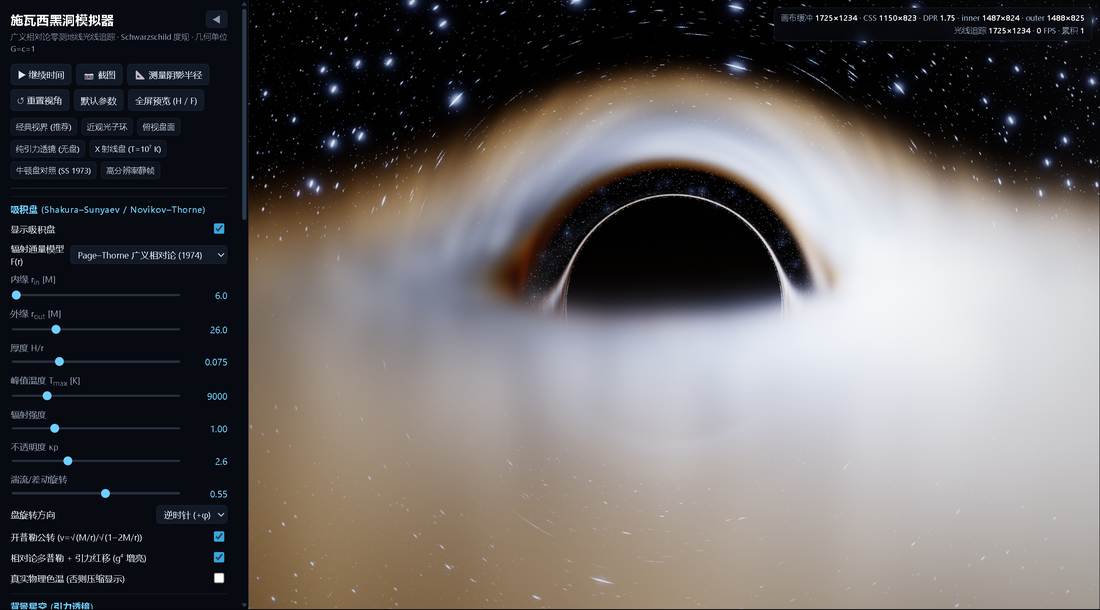
\includegraphics[width=\linewidth]{app/f21_ui_panel_open}
\caption{打包版实测：侧栏展开，画布 $1150\times823$。}
\end{subfigure}\hfill
\begin{subfigure}[b]{0.495\linewidth}
\centering
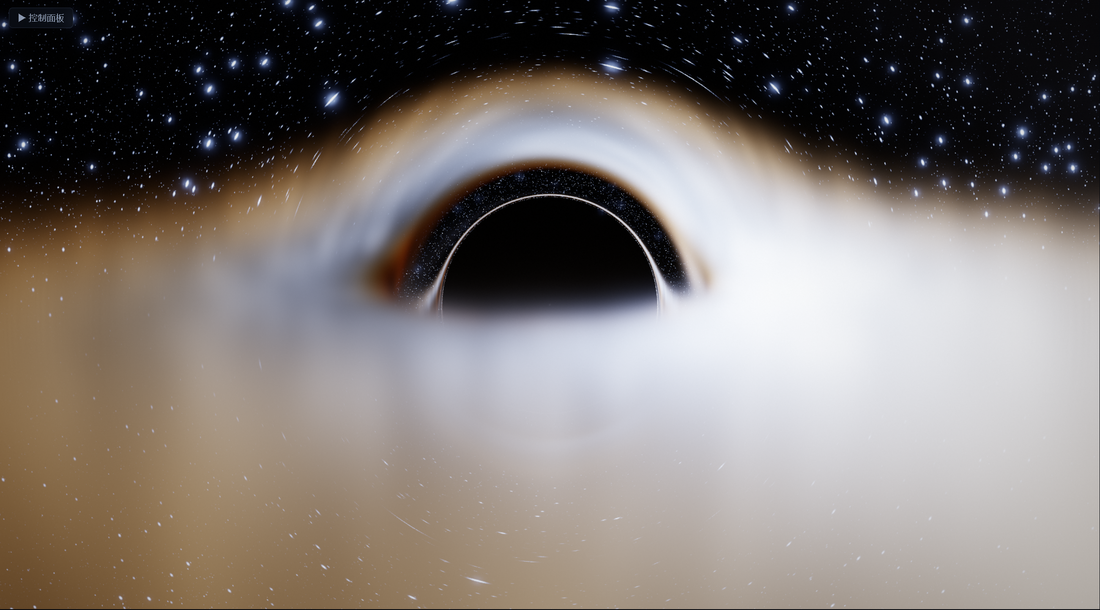
\includegraphics[width=\linewidth]{app/f21_ui_fullscreen}
\caption{打包版实测：全屏预览（\texttt{H} 键），画布 $1486\times823$。}
\end{subfigure}
\caption{程序界面（可复现产物：由 \texttt{make\_render\_figures.py} 驱动
真实渲染器截图\textbf{(b)}、\textbf{(c)} 并叠加标注\textbf{(a)}，
而非设计稿）。六个编号的含义见正文。}
\label{fig:21}
\end{figure}


\end{document}
